\documentclass[a4paper,11pt,ja=standard]{ltjsarticle}

% --- パッケージ設定 ---
\usepackage{luatexja-preset}
\usepackage{etoolbox}

% セクション番号を「第1章」形式に変更(全角数字)
\newcommand{\zenkakuNum}[1]{%
  \ifcase#1 0\or 1\or 2\or 3\or 4\or 5\or 6\or 7\or 8\or 9\fi%
}
\renewcommand{\presectionname}{第}
\renewcommand{\postsectionname}{章}
\renewcommand{\thesection}{\arabic{section}}
\makeatletter
\renewcommand{\@seccntformat}[1]{%
  \ifstrequal{#1}{section}{%
    \presectionname\zenkakuNum{\csname the#1\endcsname}\postsectionname\quad%
  }{%
    \csname the#1\endcsname\quad%
  }%
}
\makeatother

% 目次でも「第1章」形式で表示
\usepackage{tocloft}
\renewcommand{\cftsecpresnum}{第}
\renewcommand{\cftsecaftersnum}{章}
\newcommand{\tocseczenkaku}[1]{\zenkakuNum{#1}}
\makeatletter
\g@addto@macro\cftsecpresnum{\tocseczenkaku}
\makeatother
\setlength{\cftsecnumwidth}{4em}
\usepackage[top=40mm, bottom=40mm, left=35mm, right=35mm]{geometry}
\usepackage{graphicx}
\usepackage{float}
\usepackage{url}
\usepackage{caption}
\usepackage{booktabs}
\usepackage{amsmath}
\usepackage{amssymb}
\usepackage{tabularx}

\usepackage[backend=biber, style=authoryear-comp, sorting=nyt,
  maxcitenames=2, mincitenames=1, uniquelist=false,
  maxbibnames=99, minbibnames=99,
  doi=false, url=false, isbn=false, eprint=false]{biblatex}

\newcounter{figpart}
\renewcommand{\thefigpart}{\thefigure-\arabic{figpart}}

% ★これが無いと biblatex はデータを読めずエラー側に倒れる
\addbibresource{references.bib}

% 引用を角括弧にする [Author, Year]
\renewcommand{\mkbibparens}[1]{[#1]}
\let\cite\parencite

% 引用文献リストのカスタマイズ
\DeclareFieldFormat[article,inbook,incollection,inproceedings,patent,thesis,unpublished]{title}{#1}
\DeclareFieldFormat[misc,book,report,techreport]{title}{\textit{#1}}
\AtEveryBibitem{\clearfield{abstract}}

% --- bibliography の体裁(ハンギング+行間)
\setlength{\bibhang}{2\zw}                 % 2emだと日本語では差が見えにくい
\setlength{\bibitemsep}{0.5\baselineskip}  % em より安定
\setlength{\bibparsep}{0pt}

\defbibenvironment{bibliography}
  {\list{}
     {\setlength{\leftmargin}{\bibhang}%
      \setlength{\itemindent}{-\leftmargin}%
      \setlength{\itemsep}{\bibitemsep}%
      \setlength{\parsep}{\bibparsep}%
      \setlength{\topsep}{0pt}%
      \renewcommand*{\makelabel}[1]{}}}
  {\endlist}
  {\item\relax}

% --- hyperref は biblatex の後が推奨
\usepackage{hyperref}
\hypersetup{
  colorlinks=true,
  linkcolor=blue,
  citecolor=black,
  urlcolor=blue
}

\captionsetup[figure]{labelsep=period, font=normalsize}

% 番号なしサブセクションを目次に載せるコマンド
\newcommand{\figsubsection}[1]{%
  \subsection*{#1}%
  \addcontentsline{toc}{subsection}{#1}%
}


% ===== 表紙=====
\newcommand{\ThesisTitle}{%
  クラウドソーシングとデータ合成を用いた \\
  Ground Truthアセンブルスキーム:\\
  マウス全脳イメージングデータ解析における \\ 
  陽性細胞検出への適用
}
\newcommand{\AffiliationLineA}{京都大学総合人間学部 自然科学系}
\newcommand{\AffiliationLineB}{学籍番号 6100347151\quad 岡田 優真}
\newcommand{\AdvisorLine}{指導教員\quad 今吉格}
\newcommand{\SubmitDate}{2026年1月20日}

\begin{document}

\begin{titlepage}
  \thispagestyle{empty}
  \centering

  \vspace*{0.34\textheight}

  {\fontsize{18pt}{26pt}\selectfont \ThesisTitle\par}

  \vspace{18mm}

  {\normalsize \AffiliationLineA\par}
  {\normalsize \AffiliationLineB\par}

  \vspace{10mm}

  {\normalsize \AdvisorLine\par}

  \vspace{10mm}

  {\normalsize \SubmitDate\par}

  \vfill
\end{titlepage}

\begingroup
\hypersetup{linkcolor=black}
\tableofcontents
\endgroup
\newpage

% --- 要旨 ---
\thispagestyle{plain}
\addcontentsline{toc}{section}{要旨}
\begin{center}
  {\Huge \bfseries 要旨}
\end{center}
\vspace{10mm}

\noindent
生物学における大規模データの定量的解析では,深層学習は不可欠なツールとなっている.例えば,マウス全脳イメージングのような大規模のデータから生物学的な知見を抽出するためには,標識された個々の細胞を全脳スケールで網羅的に検出するために用いられ,その分布を定量化における重要な役割を担っている.しかし,深層学習モデルの性能は学習データの質と量に強く依存するにもかかわらず,こうした生物画像解析においては,専門家による手作業でのアノテーションのみによって信頼性の高いGround Truth(GT)を十分に確保することは,時間的および人的コストの観点から困難である.また,細胞の境界や判別の曖昧さに起因するアノテータ間の判断の揺らぎやバイアスが,作成された教師データの客観性を損なうという問題も存在する.そこで本研究では,これらの課題を解決するため,クラウドソーシングとデータ合成を組み合わせた高品質かつ高効率なGTのアセンブルスキームを提案し,その有効性を検証するため,全脳イメージングシステムFASTdを用いて取得されたFL3/RFPマウスの全脳イメージングデータにおける蛍光陽性細胞検出を具体的なタスクとして設定した.提案スキームは,市民科学型のクラウドソーシングによるアノテーション収集と深層学習による合成データの作成からなる.アノテーション収集では,非専門家を含む多数のワーカに細胞中心をクリックさせるタスクを提示し,得られた回答に潜在クラスモデルを適用し,ワーカの能力を推定し,その能力に応じて重み付けを行うことで,点アノテーションから,各画素が細胞重心である確率を表現したGTを整備した.合成データの生成においては,画像の特徴を学習した生成モデルを用いることで,細胞の配置情報とそれに対応する合成画像が生成され,GTの量が補完された.これらのアプローチで構築された統合GTを用いて,細胞検出モデルを訓練し,その性能を評価した結果,得られた統合GTは,専門家による判断と整合し,これを教師データとして学習を行ったモデルは,合成データのみで学習した場合と比較して,検出精度の向上が確認された.これらの結果から,提案手法はGTの構築を群衆と計算機に委ねることで,コストと品質のトレードオフを解消しうることが示唆された.また,アノテーションの統合プロセスが,個々の判断のばらつきを確率的な確信度へと変換し,モデルが学習すべき特徴が自然に抽出される可能性も示された.本研究で提案されたスキームは,特定の専門家や既存データセットのバイアスに依存せず,対象ドメインの生データから低コストで高い真正性を持つGTを構築する手法を提供するものである.これは,GT の整備が運用上の課題となっている,深層学習を用いた医学・生物学的画像解析の実用性と信頼性を底上げする汎用的な基盤となることが期待される.



\newpage


\section{序論}

\begin{quote}
  \itshape
  ``Data-centric AI is the discipline of systematically engineering the data needed to successfully build an AI system.''
  \upshape

  —アンドリュー・ン (2022)
\end{quote}

\vspace{1em}

深層学習の隆盛は,しばしば高性能なアーキテクチャや大規模計算資源の発展として語られてきた.しかし ,深層学習システムの成否はモデル設計だけでなく,学習に用いるデータをどのように設計し,整備し,運用可能な形に仕立てるかにも強く依存する.すなわち,アルゴリズムと同程度か,場合によってはそれ以上に,どのようなデータをどのような形で与えるかが本質的な設計変数となっている.

機械学習コミュニティでは長らく,固定されたデータセットに対してモデルのアーキテクチャやハイパーパラメータを改善することで性能を競う「モデル中心 (model-centric)」なアプローチが主流であった.この文脈では,モデル設計の改良が改善の主たる手段として想定されている.しかし近年,ンの定義にみられるような「データを系統的に工学する」視点をより積極的に受け止め,モデル側をある程度固定したうえで,ラベルの一貫性やデータ分布の代表性,アノテーション手順そのものを系統的に設計・改善することで性能と信頼性を高めようとする「データ中心 (data-centric)」のパラダイムが提案されている [Jakubik et al., 2024].NeurIPSにおけるData-Centric AI WorkshopやDatasets and Benchmarksトラックの新設は,教師データやデータワークフローの設計それ自体が独立した研究対象として可視化されつつあることを象徴している [NeurIPS, 2021].

本研究では,Data-centricパラダイムのもと,マウスの全脳イメージングデータ解析における蛍光陽性細胞の検出精度向上を目的とした,Ground Truth(GT)データセットのアセンブルスキームを提案する(図\ref{fig:fig1}).ここでアセンブルとはデータの収集,整備からデータセットの構築までを指し,Ground Truthを,教師あり学習で用いる学習ターゲット,および性能評価で参照するラベルの両方を含む,ラベル付きデータの総称として用いる.

本研究で構築した GT データセットは,マウスの全脳イメージングデータにおける陽性細胞の位置座標の集合である.クラウドソーシングを用いた市民科学的アプローチによって,専門家と非専門家を含む N 人のワーカによる陽性細胞のアノテーションを収集し,各ワーカの能力で重み付けることで,真の陽性細胞の座標を推定した.このデータセットのサブセットを学習データとして画像生成器を訓練し,陽性細胞の合成画像を生成し,GT データセットに加え,そのサイズと多様性の向上を図った.提案スキームで構築された GT データセットの効果を評価するため,既存のモデルと,GT データセットの異なる割合のサブセットを用いて訓練された深層学習モデルで,陽性細胞の検出精度を算出した.装置構成等の撮像方法の詳細は,第5章にまとめる.

\subsection{全脳イメージングデータ解析のボトルネック}

近年,脳全体の構造や活動を計測する全脳イメージング技術は急速に発展している.マウスを対象とした三次元全脳イメージングでは,大きく二つの技術的ルートが確立されてい つつある [Osten and Margrie, 2013; Ueda et al., 2020b; Jiang et al., 2023].

第一のアプローチは,iDISCO,CUBIC,CLARITYなどの組織透明化プロトコルとライトシート蛍光顕微鏡を組み合わせる手法である [Chung et al., 2013; Renier et al., 2014; Susaki et al., 2014; Ueda et al., 2020a].組織を透明化することで物理的な切断を行うことなくマウス全脳を撮像し,数十 µm オーダーの空間解像度で三次元空間にマッピングすることが可能になった.第二のアプローチは,連続切片イメージングである.これは脳ブロックを自動的に薄切しながら各切片表面を高解像度顕微鏡で撮像し,得られた連続断面画像から三次元全脳画像を再構成する手法であり,STPT(Serial Two-Photon Tomography)などが代表的である [Ragan et al., 2012; Gong et al., 2013; Ueda et al., 2020b].

本研究では,全脳蛍光イメージングデータを,後者に属する高速・高精細全脳イメージング装置 FAST(block-face serial microscopy tomography)の改良版FASTdで取得した.FAST は,スピニングディスク共焦点顕微鏡,自動リニアスライサー,電動ステージを一体化することで,成体マウス全脳を 0.7 µm × 0.7 µm × 5 µm の空間解像度で約 2.4 時間という短時間で撮像できる.FASTd は FASTの構成を踏襲しつつ,その共焦点スキャナユニットをより感度の高いものに換装し,数 µm オーダーのボクセルサイズで高速・高解像度での撮像を実現している.こうしたex vivo全脳イメージングでは,マウス脳1サンプルあたり100 GBから数十TBに及ぶ高次元データが生成され [Ueda et al., 2020b],個体全脳にわたる蛍光陽性細胞の分布を網羅的に観察できる.

しかし,取得されるデータは連続的な蛍光強度分布に過ぎず,「どの脳領域にどのような細胞が存在するか」「どの脳領域がどの程度活動したか」といった生物学的に意味のある情報は,このデータから計算機的な画像解析を介して初めて抽出される.

一般に,全脳イメージングデータを構造化データへ変換するには,(i) 画像中から蛍光陽性細胞を検出して個々の三次元座標を求める処理と,(ii) 得られた細胞座標を Allen Mouse Brain Atlas CCFv3 などの標準脳座標系に非線形変換によって写像し,各細胞に脳領域ラベルを付与する処理(registration)が必要である [Wang et al., 2020; Avants et al., 2011].両者を統合することで,全脳スケールで位置情報と領域情報を付与された陽性細胞のデータベースが構築される.

実際に,ClearMap をはじめとする画像処理パイプラインは,免疫染色された c-Fos 等の最初期遺伝子発現の全脳マッピングに広く用いられてきた [Renier et al., 2016; Sommer et al., 2011; Berg et al., 2019; Kaltenecker et al., 2024; Ueda et al., 2020b].これらの多くは,閾値やフィルタを用いたヒューリスティックな手法か, ilastik に代表される機械学習手法によって細胞を検出し,重心座標を計算したうえで標準脳アトラスに registration し,脳領域アノテーションを付与する.

より高精度でロバストな陽性細胞検出を指向して,近年では深層学習器を用いた自動細胞検出が全脳イメージングデータ解析における事実上の標準になりつつある.畳み込みニューラルネットワーク(Convolutional Neural Network; CNN)やその一種であるU-Net系のモデルは,高次元画像から特徴量を自動抽出し,局所的なパターンの違いを学習によって獲得できるため,蛍光強度やノイズパターンの多様性に対して高いロバスト性を示し,従来手法に比べて細胞検出性能を大きく向上させてきた [Ronneberger et al., 2015; Çiçek et al., 2016; Moen et al., 2019].近年では,テラボクセルスケールの全脳蛍光イメージングデータを対象に,三次元深層学習による細胞セグメンテーション,標準脳への registration,および空間統計解析を一体化したパイプラインも提案されており,MIRACL-ACE はその代表例である [Attarpour et al., 2025].このようなパイプラインによって,全脳イメージングデータは高解像度の画像から座標付きの細胞点群へと変換され,領域別の細胞数や細胞密度,マーカー陽性細胞の分布などを全脳スケールで定量化可能となる.このように全脳イメージングデータを解析することで, 例えば,学習課題の訓練前後で c-Fos 陽性細胞の分布を比較することにより,全脳スケールでその個体の経験に依存した活動変化を同定できる [Renier et al., 2016; Ueda et al., 2020b].また,遺伝子改変マウスや薬理操作における表現型解析では,その操作がどの脳領域のどの程度の細胞集団に影響を与えるかを細胞レベルで評価することが可能になる.したがって,全脳蛍光イメージングにおける蛍光陽性細胞検出は,単に画像処理上の前処理にとどまらず,行動・回路・分子の対応関係を記述するうえで不可欠な処理過程である.

一方で,このようなパイプラインにおいても蛍光陽性細胞検出は依然として重大な課題である.脳深部における信号対雑音比の低下,光の散乱や収差による像のぼやけ,透明化・固定・染色条件の差異に起因する背景ノイズの不均一性や組織変形など,生物学的画像には多くのアーチファクトが含まれる.そのため,単純な閾値処理やモルフォロジー演算に基づく古典的手法では,細胞検出における偽陽性(過検出)および偽陰性(過少検出)が無視できないレベルで生じる [Ueda et al., 2020b; Renier et al., 2016].特に,細胞が密に集積する領域や,核内と細胞質でマーカー局在が異なる領域では,「どこまでを一つの細胞とみなすか」,「重なり合う信号をいかに分離するか」といった判断が難しい.免疫染色標本における核カウントでは,手作業による計数が時間集約的であるだけでなく,観察者内および観察者間で判定の不一致が生じることが指摘されてきた [Warfield et al., 2004; Litjens et al., 2017].さらに,c-Fos マッピングなどでは単一個体あたりの陽性細胞数が膨大になるため [Renier et al., 2016; Ueda et al., 2020b],エキスパートが全脳三次元画像を目視で確認しながら一貫してラベリングすることは,事実上不可能である.深層学習に基づく自動検出器はこうした問題を大幅に緩和しうる一方で,その性能と信頼性は最終的に,限られたリソースのもとでどのようにラベルを収集し,不確実性をどう扱いGround Truthデータセットを構築するかに強く依存している.したがって,より高精度な細胞検出が可能な深層学習モデルを構築するには,モデルの改良と並行して,「どのようにして良いGround Truthを準備するか」というデータ側の課題を解消する必要がある.

\subsection{生物学的データにおける教師データ作成の課題}

深層学習モデルが性能を発揮するためには,大量かつ高品質なデータセットが不可欠である [Litjens et al., 2017; Tajbakhsh et al., 2020].専門家が詳細な手作業アノテーションによって作成したラベルデータセットは gold standard,既存アルゴリズムの出力や複数の観察者のラベルを集約することで得られたラベルデータセットは silver standard に分類される [Lehmann et al., 2002; Lucena et al., 2017; Lucena et al., 2019].gold standard データセットを用いることは理想的ではあるものの [Lehmann et al., 2002],医用・生物学的イメージングでは,gold standard データセットの作成コストが極めて高く,ピクセルレベルのラベル付けは時間的コストが大きい [Lucena et al., 2017; Lucena et al., 2019; Wang et al., 2021].その結果,公開ベンチマークは特定の臓器や撮像法に偏り,規模の小さいデータセットを対象とした研究が増加する [Litjens et al., 2017; Tajbakhsh et al., 2020].本研究が対象とするような,単一個体あたりテラボクセルスケールの 全脳イメージングデータでも,「一画素ごとに正解ラベルを付与する」という従来的な意味での教師データ整備は実際的には不可能に近い.そのため,一部の条件を緩める代わりにスケール性や実用性を高めた silver standard データセットも併用することが現実的である.実際に,脳 MRI のskull-strippingにおいてLucenaらは,専門家による手動セグメンテーションをgold standardとみなしつつ,複数の自動抽出アルゴリズムの合意から得られたマスクをsilver standard masksとして定義し,後者のみを用いて深層学習モデルを訓練している [Lucena et al., 2017; Lucena et al., 2019].

全脳イメージング解析パイプライン MIRACL–ACE でも,全脳三次元画像に対する教師ラベルを,純粋な専門家手動アノテーションで作るのではなく,既存の自動セグメンテーション出力を起点に半自動的に整備しており,著者らはこの種の教師ラベルを gold standard ではなく silver standard と位置づけている [Attarpour et al., 2025].具体的には,脳画像から小さなパッチを切り出し,自動手法で得たセグメンテーション結果を手動アノテーションの代替として用いつつ学習データを整備し,その一部を専門家が目視で点検して,誤検出や境界のずれが疑われる箇所について教師ラベル(セグメンテーション結果として付与された領域ラベル)を修正する段階的なワークフローを採用している.そこでは,教師データは「全ボクセルを人手でアノテートした理想的なgold standard」ではなく,「自動セグメンテーションと部分的な専門家チェックを組み合わせて得られた近似的な参照ラベル」,すなわち silver standard で構成されていると言える.これは,アノテーションの時間的コストを削減するための合理的な設計である一方で,アルゴリズム由来のバイアスと,人手による確認が及んでいない領域に残存する誤りを教師データに内包する可能性がある.

さらに,アノテータ自体の不確実性に大きく影響される点も,とりわけ生物学におけるデータセットの無視できない特徴である.免疫染色標本における核カウントの研究では,観察者内・観察者間のばらつきが定量化されており,手作業であっても真の細胞を一意に定めることは困難である [Shu et al., 2020].多くの深層学習モデルは単一のgold standardラベルを正解として学習するが,現実にはラベルは観察者や条件に依存する.

近年では,多アノテータによる教師データ(Ground Truth)の構築において,ラベル統合(label fusion)によって不一致ラベルを単一の真値で代表してよいのかは,モデル予測の不確実性推定,とりわけそこに専門家間の不一致がどれだけ反映されているか,と不可分であることが示されている.Jungoらは医用画像セグメンテーションを対象に,多数決などでラベル統合を行う設定と,複数アノテータのラベルをそのまま学習に用いる設定(no fusion)を比較し,統合ラベルで学習したモデルは専門家間の不一致の大きい領域で不確実性を過小評価しやすい一方,no fusion では,専門家間の不一致をよりよく反映した不確実性を加味できることを示した.さらに,この改善はセグメンテーション精度を大きく損なわずに得られる場合があると報告している [Jungo et al., 2018].全脳イメージングにおける細胞検出においても,「どこまでを一細胞とみなすか」「重なり合うシグナルをどのように分離するか」といった判断には本質的な曖昧さが含まれており,ノイズとバイアスが教師データに含まれることは避けられない.MIRACL–ACEのようなsilver standardに基づくパイプラインでは,アルゴリズム由来の一貫した揺らぎとアノテータ由来の多様な揺らぎがともにラベルに含まれるが,その不確実性がモデルの学習と推論に明示的に反映されているとは限らない.

こうした制約を緩和する手段として,データ拡張 (data augmentation) や生成モデルを用いた教師データの拡充も検討されている.従来の幾何学変換や強度変調に加え,Generative Adversarial Network(GAN) やDiffusionモデルによる画像生成・変換は,医用画像においてもデータ拡張・ドメイン適応・ノイズ除去などに応用されつつある [Yi et al., 2019].これらは限られたデータから多様な訓練サンプルを合成することで,アノテーションにかかる時間的なコストを間接的に緩和しうる一方で,学習データに含まれるバイアスを増幅させる危険性や,生物学的にあり得ない構造 (hallucination) を生成するリスクを内包しており,生成されたラベルをどこまで信頼できる教師データとみなせるかについては慎重な議論が必要である.

以上のように,深層学習は全脳イメージングにおいてマーカー陽性細胞検出のための協力な道具となるが,その性能は訓練,テストデータセットの「量」(どれだけ作成することができるか),「質」(どれだけ誤りやバイアスを排せるか),「一貫性」(アノテータや条件による揺らぎをどこまで減らせるか)に依存している.MIRACL-ACEのような最先端のパイプラインにおいてすら,アノテーションの時間的コスト,アルゴリズムに由来するバイアス,アノテータ感の揺らぎをどのように扱うか,という問題は十分に解決されていない [Attarpour et al., 2025; Warfield et al., 2004; Jungo et al., 2018].

\subsection{市民科学型のクラウドソーシングによる画像アノテーションデータセットの整備}

質と量を担保してGround Truthデータセットを構築するアプローチとして,ヒューマンコンピューテーションが有用である.ヒューマンコンピューテーションは,人間によっては容易だが,コンピューターのみでは解決の難しい課題を,人間の能力と組み合わせることで解決を図る手法である [Kashima et al., 2016].本研究では,ヒューマンコンピューテーションを実施するプラットフォームとして,市民科学(Citizen Science)によるクラウドソーシングに注目した.市民科学とは,専門家ではないボランティアが科学研究に参加し,観測・分類・データ解析などのタスクを担う枠組みであり,生態学や天文学,環境科学などの分野で大規模な成果を挙げてきた [Bonney et al., 2009].クラウドソーシングとはインターネットを介して不特定多数の参加者(crowd)にタスクを提示し,作業を分担してもらう仕組みであり,ヒューマンコンピューティングの実装形態の一つとして,「多数の人に小さな作業を割り振って集約する」ための基盤として用いられる [Kashima et al., 2016].

代表例であるGalaxy Zooプロジェクトでは,図\ref{fig:fig2}に示すようなWebインタフェースを通じて天文画像中の銀河形態をボランティアが視覚的に分類し,数十万人規模の参加者から数千万件を超えるアノテーションを収集することに成功している [Lintott et al., 2008; Willett et al., 2013].このプロジェクトでは,(i) 一つの対象(銀河)に対して多数の独立したアノテータから回答を集め,個々の誤りを平均化し,(ii) アノテータの過去の回答履歴から各アノテータの信頼度を推定し重み付き集約を行う,という二つのプロセスによって,専門家に匹敵する精度の銀河形態カタログを構築している.Zooniverseはこのコンセプトを一般化し,画像分類・時系列イベント同定・音声ラベリングなど様々な科学プロジェクトにおける大規模クラウドアノテーションのプラットフォームとなっている [Simpson et al., 2014].このように,クラウドソーシングに基づく多数決と重み付けによる統合により得られるラベルは,gold standardに匹敵するGround Truthの一種として位置付けることができる.

医用・生物学的イメージングにおいても,専門家によるアノテーションを補完・拡張する手段としてクラウドソーシングの導入が検討されている.例えば,網膜眼底画像中の病変グレーディング [Mitry et al., 2016] や脳画像中の腫瘍領域同定 [Amgad et al., 2019] では,ウェブインターフェースを通じて多数のアノテータから回答を収集し,適切な品質管理を行うことで専門家によるアノテーションと遜色ない精度を達成可能であることが示唆されてきた.

これらの研究に共通するのは,アノテーションにかかる作業を単純化したマイクロタスクや,難易度調整, や品質管理 (事前に専門家による基準解が設定されたタスクでの回答の収集やアノテータのスクリーニングなど) を設計し,組み合わせることで,非専門家を含む集団から有用な教師データを抽出している点である.

古典的な多数決や単純平均によるアノテーションの集約は,アノテータの能力差や,誤りの偏りを考慮しない一様重み付けに基づく集約則であり,アノテータ間のばらつきが小さい場合には有効である.しかし,バイアスを持つアノテータが多数含まれる場合などには,誤ったデータが集約により生成される危険性があることが指摘されている [Warfield et al., 2004].これに対し,STAPLEなどの潜在クラスモデルに基づく回答の集約は,各アノテータを感度・特異度を持つノイズ付き観測器としてモデリングし,EM アルゴリズムを通じて「真のラベル分布」と「アノテータ性能」を同時推定する [Warfield et al., 2004; Litjens et al., 2017].

\subsection{小括}

全脳蛍光イメージング解析において高精度陽性細胞検出モデルは必須であり,そのようなモデルには質良ともに優れた GT データセット(e.g. 陽性細胞の座標)が不可欠である. そこで本研究では,最初に市民科学型クラウドソーシングを用いて,専門家や非専門家を含む多数のアノテータによる,全脳イメージングデータからの陽性細胞のアノテーションデータを収集した.このタスクは,適切なインターフェース設計と簡潔な指示があれば非専門家でも一定の精度で遂行できる視覚的課題であり,クラウドソーシングに適していると考えられる.一方で,少数の専門家だけで行うことは非現実的である.

次に,多数のアノテータが独立に打点した細胞の座標から合意点(i.e., 細胞の真の座標)を求めるために,打点のクラスタリングを通じて細胞候補のクラスタを抽出し,多数のアノテータが独立に打点した細胞の座標をクラスタリングし,ラベル融合モデル STAPLE [Warfield et al., 2004] を用いて合意点(i.e., 細胞の真の座標)とアノテータの能力を同時に推定した.これにより,観察者の能力で重み付けられた合意点からなる GT データセットが構築された.この GT データセットの一部を用いて画像合成器を訓練し,GT データセットの画像特徴を模倣した合成画像を生成し,GT データセットに追加することで,その量と多様性の向上を図った.

最後に,この GT データセットを用いて CenterNetアーキテクチャ [Zhou et al., 2019] を採用した深層学習ベースの陽性細胞検出モデルを訓練した.GT データセットの別のサブセットをテストデータとして,それらのモデルと既存のモデルの精度を評価した.

以上を通して,アノテーションに内在する不確実性を考慮した Ground Truth データセットの構築スキームとパイプラインを提案し,それが,頑健な細胞検出モデルの構築に貢献しうるかどうかを検証した.

\clearpage
\section{方法}

\subsection{提案手法の概要}
本研究では,Arc プロモーター下で Venus を発現するレポーター由来のマウス全脳イメージングデータを対象として,マーカー陽性細胞検出器を訓練するための Ground Truth を真正性を維持しつつ,効率よく構築するスキームを提案し,その運用に必要なパイプラインを実装した(図\ref{fig:fig3}).全脳イメージングデータを取得した実験の詳細は第5章に記載する.

提案スキームは,対象画像の抽出,二系統の Ground Truth 作成,GT による検出器の訓練からなる.その独自性は,クラウドソーシング由来のアノテーションと条件付き生成モデルによる合成データを併用することでアノテーションコストを抑えつつ,全脳イメージングデータに含まれる陽性細胞の検出器のための Ground Truth を拡充する点にある.

まず対象画像の抽出では,全脳画像から関心領域に対応する画像部分を取り出し,提示単位を揃えるために画像をタイル化する.続いて,背景が大半で蛍光信号がほとんど含まれず,陽性細胞が出現しにくいと見込まれるタイルを除外する簡易な選別を行い,アノテーションと検出器の学習に用いる画像を整える.この段階により,後続のアノテーション作業の負担とばらつきを抑えつつ,検出器が学習すべき画像パターンに集中できるようにする.対象画像の抽出手順と基準は 2.3 節で述べる.

次に,Ground Truth を,二つの経路で構築した.第一の経路では,クラウドソーシングで,タイル画像上でマーカー陽性細胞の中心をクリックする形式でアノテーションを収集した.ここでは同一タイルに対して複数のワーカを割り当て,冗長な観測を得ることで,個々のクリックに含まれるずれや見落としを統計的に扱えるようにした.アノテーション収集の仕組みと運用は 2.3 節で述べる.しかし収集されたクリック座標は,同一細胞に対して複数のクリックが発生し,さらにアノテータごとに誤差の傾向も異なるため,そのままでは GT として利用できない.そこでクリック群を統合し,同一細胞の候補を推定した上で,統計モデルを用いて,陽性細胞の座標とワーカそれぞれの信頼度を推定し,アノテーションを集約した.この処理により,各陽性細胞の中心座標を確定的な一点として与えるのではなく,アノテーションのばらつきを反映した空間的な確率分布として表現した GT を得た.統計モデルと Ground Truth への変換手順は 2.4 節で述べる.

第二の経路では,抽出した対象画像を模倣する条件付き画像生成器を訓練し,合成画像を生成する.生成器は局所コントラストなどの画像特徴を学習し,対象データに類似した画像を出力することを目指した.この経路の重要な点は,合成画像と同時に Ground Truth を生成できるように設計できることである.本研究では合成時に細胞中心の配置を明示的に生成し,その配置に整合する画像を生成することで,追加のアノテーションなしに教師信号付きデータを増やすことを可能にした.条件付き生成器の設計,学習手順,および  生成の方法は 2.5 節で述べる.

最後に,二つの経路から得られた Ground Truth を用いて検出器を訓練した.すなわち,クラウドソーシング由来の統合 GT と,画像合成由来の GT を学習データとして組み合わせる.検出器の学習設定と評価手順は,2.6 節および 2.7 節で示す.

\subsection{問題設定}

\subsubsection{出力の要件}
全脳イメージングにより得られるデータは,脳全体にわたるマーカー陽性細胞の空間分布を含む.これらのデータを用いた解析では,脳領域ごとの細胞数や密度の比較,行動実験における群間差の統計検定などが中心であり,解析の最小単位として陽性細胞の三次元空間上の位置(座標)を必要とすることが多い.実際,最初期遺伝子発現の全脳解析では,陽性細胞を自動抽出して三次元空間にマッピングし,領域別の細胞数・密度などを算出して統計的に比較するパイプラインが提案されている [Renier et al., 2016].同様に,全脳スケールの解析では,蛍光陽性細胞はピクセルレベルのマスク画像としてではなく三次元空間上の点として抽出・集約され,領域別の集計量として比較される [Osten and Margrie, 2013; Jiang et al., 2023].

ここから,本研究における細胞検出の出力を,マーカー陽性細胞の重心座標の集合と定義し,全脳イメージングデータから細胞重心を頑健に検出する問題を以下のように定式化する.

\subsubsection{問題の定式化}
入力を,適切な輝度正規化を施した3次元画像 $I$ とする.このとき出力は,陽性細胞の重心座標の集合
\begin{equation}
  P = \{ (x_i, y_i, z_i) \}_{i=1}^{N}
\end{equation}
である.ここで $N$ は陽性細胞数である.本研究の課題は,多様なノイズ,背景構造,輝度むらや細胞の密集,近接といった条件下において,$P$ を高い精度のもとで推定することである.

\subsubsection{検出手法の選択}
全脳イメージングにおける陽性細胞の推定は,画像解析の観点から Segmentation と Detection に大別できる(図\ref{fig:fig4}).Segmentation はイメージングデータ上の各ボクセル/ピクセルで「細胞/背景」などのラベルを推定し,連結成分ラベリングやインスタンスセグメンテーションにより個々の細胞領域を抽出したうえで重心座標を算出する枠組みであり,U-Net 系に代表される手法が広く用いられている.実際,NuMorph は,組織透明化データに対して 3D U-Net を用いた核セグメンテーションを組み込んでいる [Krupa et al., 2021].また,U-Net による 3D セグメンテーションをもとに,領域別の細胞数・密度の集計へ接続する設計が提案されている [Attarpour et al., 2025].一方,Detection は画像中の物体の存在位置を直接推定し,中心座標を出力する枠組みであり,全脳規模のイメージングデータから細胞位置を直接推定する深層学習アルゴリズムも提案されている [Tyson et al., 2021].

全脳解析はデータマイニングであり,細胞位置(座標)から,脳領域ごとの細胞数・密度・空間密度マップ,群間差から有用な情報を発見できれば,例えば細胞の形態のような,生物学的に詳細な情報が常に必須とは限らない.この点で,Segmentation は細胞の重心を得るために「細胞マスクの推定 $\to$ 重心推定」という段階を踏むのに対し,Detection は中心座標を直接推定できるため,推定値がそのまま後段の解析で用いられる量となり,後処理が減らせ,結果として Segmentation に比して処理の高速化につながりやすい.さらに,全脳データでは陽性細胞検出器のための Ground Truth 作成がボトルネックになりやすく [Ueda et al., 2020b; Jiang et al., 2023],アノテーションの対象がピクセル規模のマスク画像である Segmentation よりも,物体の位置を主たる GT とする Detection のほうが,データ収集コストとスケーラビリティの面で有利である.加えて,蛍光画像では境界が曖昧になりやすく,近接細胞が部分的に融合して見える場合にはマスク画像からの分離が困難であるが,中心座標等の推定に焦点を当てる設計では細胞の重心座標を直接推定するため,境界の曖昧さや融合の影響を受けにくくできる.これらの理由から,本研究は細胞重心座標の抽出という目的に対して,Detection を採用した.

Detection の設計にも複数の系統があり,代表的にはアンカーに基づく方式やアンカーフリー方式,そして中心点をキーポイントとして推定する方式がある.このうち本研究の対象は「小さく,多数で,密集しうる」細胞であり,出力として求めるのが重心座標そのものである.したがって,中心点をモデルの主要な予測対象として定義する方法は,求めたい量と,学習で最適化する量が一致するため,問題設定を最も素直に表現できる.CenterNet は物体中心をヒートマップとして推定し,必要に応じてサブピクセル補正やサイズの回帰を併用するモデルとして提案されており [Zhou et al., 2019],点アノテーションを Ground Truth として取り込める形式である.全脳データでは撮像条件や領域差により,蛍光強度だけでなく細胞像の見かけの大きさや形状も一様でない [Jiang et al., 2023].アンカーベース方式は,あらかじめ定めた候補ボックスの大きさや縦横比とのマッチングに学習が依存するため,対象物サイズ分布が変動するとアンカー設定の再調整が必要になり,性能が不安定になりやすい.これに対し,中心点表現を主とする方式は,こうした事前設計への依存が相対的に小さく,運用上の調整負担を下げやすい.以上より,本研究では中心点の直接推定する CenterNet をアーキテクチャとして採用した.ここで重要なのは,特定モデルありきで手法を組み立てるのではなく,まず全脳イメージングデータ解析の目的(細胞中心座標に基づく領域別集計・群間比較)と Ground Truth 作成における制約を整理し,そこから導かれる要件として中心座標を出力とする検出モデルを選んだ,という点である.なお,これにより,本研究では Ground Truth をボクセルマスクではなく細胞中心点(重心座標)を基本単位として設計した(以下参照).

\subsubsection{Ground Truth の要件}
Ground Truth は,二次元画像上の画像座標系における中心点 $(x, y)$ の集合として表現する.この表現は,アノテーションによって得られる場合にも,合成データ生成過程で与えられる場合にも共通であり,学習時には同一形式の GT として扱える.本研究では,検出タスクに対する Ground Truth の最小表現として,画像内座標系の中心点集合 $\{ (x, y) \}$ を一次情報として取得・保持する.これにより,例えば 3D ボリュームでの細胞検出などで空間座標が必要な場合は,画像メタデータを介して $\{ (x, y) \}$ を参照できる.

CenterNet においては,細胞の中心点はヒートマップとして表現され,検出器の訓練に用いられるため [Zhou et al., 2019],生の点座標と,学習用に変換されたターゲット表現を対応づけて保持する.ここでは中心点に付随する信頼度(重み)を保持できる構造としておくことが可能である.

図\ref{fig:fig5}に,本研究で扱う Ground Truth として,重み付きヒートマップの例を示す.

\subsection{市民科学型のクラウドソーシングによるアノテーションデータの収集}

\subsubsection{課題の設計}
全脳画像における蛍光陽性細胞の重心座標の Ground Truth を,専門家の手作業だけで供給するのは困難である.そこで本研究では,非専門家を含む多人数のワーカにアノテーションさせる市民科学型のクラウドソーシングを採用した.多数の非専門家のワーカによるラベリングを統計的にモデリングし,専門家に匹敵する頑健なカタログを構築する市民科学アプローチは,天文学における Galaxy Zoo などの十分な実績をもつ [Lintott et al., 2008; Lintott et al., 2011].例えば,非専門家によるアノテーションデータであっても,十分な量と冗長性があり,適切な集約をおこなうことで,実用的な品質のアノテーションに昇華できると報告されている [Snow et al., 2008].

クラウドソーシングにおける最大の課題は,参加者あたりの認知負荷と作業時間を抑えつつ,目的に整合したラベルデータを回収する点にある [Quinn and Bederson, 2011].本研究で必要な Ground Truth は細胞の位置であり,画素単位の境界マスクではないため,タスクは細胞と思われる範囲の中心をクリックする点アノテーションとして設計できる.点ラベルアノテーションは,マスキング等の詳細なアノテーションと比べて作業にかかる労力が低い一方で,学習に有効な信号を与えうることが,コンピュータビジョン分野で示されている [Papadopoulos et al., 2017].顕微鏡画像においても,点アノテーションを用いた弱教師ありの細胞セグメンテーションが提案されており,マスキングなどと比べてアノテーションの負担を大きく削減しうるという報告がある [Khalid et al., 2023].したがって,陽性細胞の重心座標の検出器の訓練,テストデータとして,点アノテーションのデータセットは情報量とコストのバランスが取れた合理的な選択といえる.

全脳画像は高解像度かつ広範囲である.例えば FASTd で撮像した脳画像(図\ref{fig:fig30})は単一断面だけでも 4K 画像の約10枚分に相当するため,そのまま提示すると,単純な細胞検出以外に注意力,作業記憶(画像中のどの範囲まで探索したかを覚える)など,必要とされる能力が多くなる.この種の巨大画像を小領域パッチへ分割して処理・提示することは,画像解析では一般的であり,計算上の都合だけでなく,人間の作業負荷を下げるうえでも理にかなう.そこで本研究では,まず解析対象画像を $500 \times 500$ ピクセルのタイルに切り出し,さらに提示時には $80 \times 80$ ピクセルの小タイルへ分割して逐次提示する方式を採用した.小タイルを順に提示することで,アノテーションのワーカの能力依存性を抑えることを意図している.加えて,小タイル間にオーバーラップを設けることで,タイル境界で細胞が切断されることによる見落としや判断の揺れを抑える設計とした(図\ref{fig:fig6-1}).

また,ワーカの作業継続を損なう要因として,単調な反復作業による疲労や離脱がある.クラウドソーシングでは,タスクを「短い反復単位」に分解し,進捗や即時フィードバックを与える設計が参加継続に寄与しうる [Quinn and Bederson, 2011].さらに,ゲーム要素を用いて大量の注釈を自然に回収する ``Games with a Purpose'' の考え方や,科学課題をゲーム化して参加を促す取り組みが知られている [von Ahn, 2006; Cooper et al., 2010].本研究はゲーム化を目的としないが,マイクロタスクとしての継続性を向上することを狙い,UI上の操作を単純化し,クリックと遷移を中心とした軽量なループにした(図\ref{fig:fig6-2}).

\subsubsection{使用したデータ}
クラウドソーシングに供するデータは,ワーカが短時間で判断できる視覚条件を満たすだけでなく,提示される蛍光信号がレポーター由来である確度をできる限り高める必要がある.全脳イメージングでは,撮像・試料処理条件によっては自家蛍光や背景散乱,アーチファクトが残存し,輝点が必ずしも目的分子の発現を意味しない場合があるためである [Richardson et al., 2015].そこで本研究では,先行研究で Arc の誘導・発現が相対的に強く観察されることが報告されている脳領域を優先して抽出対象とした.Arc プロモーター下で Venus を発現する系は,経験依存的な Arc 転写のレポーターとして利用されてきた [Gouty-Colomer et al., 2016].また,探索や学習課題に伴う Arc の領域特異的誘導は既報であり [Vazdarjanova et al., 2006; Chiaruttini et al., 2025],本研究では,先行研究で Arc 系シグナルが観察されやすい領域を参照し,Isocortex,olfactory areas,hippocampal formation,cortical subplate,striatum の5領域をアノテーション対象として抽出した.

アノテーション用データセットを作成するために,まず全脳画像とマウス脳アトラスを対応づけ,座標から脳領域への写像テーブルを構成することで,領域ごとの画素集合を抽出した.本研究では,この座標―領域対応に基づき,複数の主要領域からアノテーション対象領域を選定し,領域別の画像集合を形成した.

次に,各領域の画像集合を格子状にクロップしてタイル化し,本研究のクラウドソーシングにおける提示単位である $500 \times 500$ タイル画像を生成した.ただし,全タイルを無差別に提示すると,ほぼ蛍光のない暗い領域やアーティファクト優勢の領域が混入し,ワーカの負担とノイズが増える.そこで,本研究では輝度分布に基づく単純なフィルタリングを適用し,極端に暗い/情報量の乏しいタイルを除外することで,提示画像の品質を揃えた(図\ref{fig:fig7}).

最後に,得られたタイル集合をワーカへ割り当てた.クラウドソーシングでは,同一タスクを複数人に割り当てて合意による頑健性を高める一方で,冗長度を過剰にすると追加回答の情報増分が小さくなり,作業時間だけが増える.そのため,冗長性の設計は重要である [Quinn and Bederson, 2011].そこで本研究では,領域ごとのタイル集合を複数のデータセットへ分割し,各ワーカがいずれかのデータセットを担当する方式とした.さらに,後段で行うアノテーションの集約においてワーカ間のばらつきを陽に扱うため,全ワーカに共通して提示する品質管理用タイルを別途用意した(図\ref{fig:fig7}).これらのタイルに対するアノテーションは,細胞座標の真値とワーカごとの信頼度を同時に推定するためのサンプリングとして位置づけた.ここで得られる信頼度推定値は,各アノテータの回答を重み付けるために用いられ,最終的な Ground Truth の構成に影響した.この重み付けと真値の推定方法は,次節2.4で詳述する.

\subsubsection{プラットフォームの設計}
本研究では,複数のワーカが同一のプロトコルでアノテーションを実施し,得られたクリックログを後段の統合処理へ直接投入できるよう,Webベースのアノテーションプラットフォームを設計・実装した(図\ref{fig:fig8}).

実装は,ブラウザをクライアントとし,サーバ側で画像配信・認証・ログ記録を担当する三層構成であった.バックエンドは Node.js と Express を用い,データベースは PostgreSQL を採用した.ユーザセッションはデータベースに保存し,ログイン状態の安定性と運用時の監査可能性(ログイン・アクセス履歴の追跡)を確保した.表示層はテンプレートエンジンにより生成し,画像配信や表示用の前処理にはサーバ側の画像処理ライブラリを用いることで,クライアント環境差による表示の揺らぎを抑える設計とした.さらに,認証・認可,セッション管理,レート制限などの基本的なセキュリティ対策を組み込み,運用上の事故(不正アクセスや過剰リクエスト等)のリスクを低減した.アプリケーションはコンテナ化し,環境変数で接続先や秘密情報(DBパスワードやセッション鍵など)を管理できる構成とすることで,研究室内外で再現可能なデプロイを容易にした(図\ref{fig:fig9}).

課題取り組みでの操作では,アカウント認証にもとづいて,割り当てられたプロジェクトの画像(タイル)が順次提示された.ワーカが画像上の対象点をクリックすると座標が記録され,そのタイルでのアノテーションが完了したことをワーカが示すと,次のタイルが自動的に提示された.このとき保存されるログは,ユーザID,画像ID,提示順序,入力座標,タイムスタンプが含まれ,ワーカごとの作業速度なども個別に解析できる設計とした.また,運用時に作業の進捗などを確認できるよう,ユーザ別・プロジェクト別の進捗を集計し,管理画面から参照可能にした.

品質管理用タイル(Quality Control; 以下 QC)を通常タイルと同一のUI・操作で提示し,タスク開始直後に集中的に実施した.本研究の QC は,統計的な合意形成モデル(2.4 節参照)に基づき,ワーカ間の一致傾向からワーカごとの陽性細胞検出における特性,すなわち感度(sensitivity)と特異度(specificity)を推定し,成績評価および重み付けに利用するための評価タスクとして位置づけられる.この推定は,参照解データとワーカごとのアノテーションデータとの距離に基づく評価のような形式でなく,全ワーカの観測が示す相互の一致・矛盾パターンを手がかりとして,ワーカ特性を推定する枠組みによって実現する.QC を運用の初期段階で集中的に提示する利点は,評価に必要な観測を早期に確保できることに加え,QC 実施後に課題を途中で中断したワーカであっても,推定に必要な QC 応答が得られていれば,当該ワーカが提出した通常タイルのクリックログを推定された特性に基づいて重み付けし,解析に取り込める点にある.QC をランダムに挿入する設計では,中断したワーカが十分な QC に遭遇しない可能性があり,その場合にはワーカ特性を推定できず,結果として当該ワーカのアノテーションデータ全体を除外せざるを得ないリスクを伴う.また,クラウドソーシングにおける品質管理は一般に有効だが,少数の評価用タスクが反復提示されるという性質を利用し,複数ワーカが外部チャネルで情報を共有して評価用タスクを識別し,当該部分のみ慎重に回答することで検査を回避する,といった共謀に基づく敵対的操作が指摘されている [Checco et al., 2018; Checco and Demartini, 2020].そこで本研究では,QC 用タイルと通常タイルを区別しない形でワーカに提示し,解析時に QC 用タイルのデータのみを用いることで,評価タスクとしての役割とリスクへの対応を両立させた.

データ運用の観点では,画像の取り込みから提示までの経路を明確化し,追加の画像の投入やアノテーションの再収集が容易な構成とした.具体的には,新規画像を所定ディレクトリへ配置すると自動的に検出してデータベースに登録する仕組みと,必要に応じて手動スキャンで画像登録を実行する手段を併設し,データ追加の運用負担を軽減した.画像はプロジェクト単位で整理され,アノテーション対象の画像やデータ出力を独立に保持・管理できるようディレクトリ構造を設計した.さらに,データベース初期化,画像のデータベースへの登録,アノテーションのエクスポート等をユーティリティとして整備し,運用者が収集状況に応じて管理作業を実行できるようにした.加えて,本システムを異なる環境や対象に活用することを想定し,リバースプロキシの利用やバックアップ手順を想定し,ログ監視・データベースダンプ・データディレクトリのアーカイブなど,研究データとしての保存性を担保するための方法をリポジトリに併記した.以上により,本研究のクラウドソーシングは,単発の作業募集に留まらず,アノテーションを収集し,統合し,それを用いた結果から必要に応じて追加のアノテーションを再度収集するという反復的運用を可能にする.

\subsubsection{ワーカの募集と運用}
ワーカは二つの母集団から募集した.第一に,研究室内メンバーからランダムに抽出された 25名が参加した.第二に,2025 年度「実験系生物学者のための数理・統計・計算生物学入門」の受講者26名が参加した.参加条件は,Web ブラウザを介して本プラットフォームへアクセスでき,画面上の画像に対してクリック入力を行えることであり,視認・入力に支障のある者は含まれていなかった.参加者は不利益なくいつでも課題を辞めることができた.

アノテーション実施期間は 2025年11月18日から 2026年1月7日とした.アノテーション用サイト上でユーザ登録を行う際に,「本サービスで取得されるデータが,個人を識別できない形に加工された上で学術研究に利用されること」に同意する旨のチェックボックスを設け,これにチェックしたワーカのみが課題に参加した.登録ユーザ名は本名である必要がなく,ワーカが個人を特定されにくい識別子を用いて参加できるようにした.ワーカは各自の都合のよい時間に PC,スマートフォン,タブレット等からプラットフォームへアクセスし,割り当てられた画像集合に対してアノテーションを行った.ワーカごとに割当データセットを固定し,提示順序と入力ログ形式を統一した.入力はクリック座標として記録され,ユーザID,画像識別子,提示順序,タイムスタンプ等のメタデータとともにデータベースへ保存された.これ以外のワーカの情報(年齢,性別,外見,賞罰など)は収集されなかった.

インストラクションは,ワーカにバイアスを与えないよう,かつ短時間で作業を開始できることを優先して必要最小限にした.細胞中心点の判断は,実験系・撮像条件・背景構造に依存した曖昧さを含みうるため,事前に細則を与えすぎると,ワーカの解釈に基づくバイアスが生じ,自然な回答,すなわち,どのような対象を細胞と判断するのか,が抑制される可能性がある.そこで本研究では,操作定義(対象と思われる輝点の中心を一点でクリックする)と少数の例示にとどめ,個々の判断の揺れは後段の統合処理で扱う方針とした.多数参加型プロジェクトでは,簡潔なガイドを与えた上で反復的に分類を集め,集約によって安定した推定を得る運用が成立しうることが市民科学の分野において報告されている [Lintott et al., 2008; Lintott et al., 2011].

\subsection{アノテーションの統合}
2.3節のプラットフォームから得られるアノテーションは,同一画像に対する複数ワーカを含むが,そのままでは学習・評価に用いる Ground Truth として使用できない.アノテーション統合の目的は,点アノテーション集合から,より確からしい細胞中心位置をコードする GT を構成することである.このとき,解くべき問題は少なくとも以下の二つである.

第一に,ワーカの能力推定に関する問題である.ワーカは細胞を見落とすことがあり,逆に背景の輝点やノイズを細胞としてクリックすることもある.陽性細胞の座標をワーカの単純な多数決によって求めるにはワーカの誤りが同程度で独立,かつ対象の出現頻度や難度が極端でないことが暗黙に要請されるが,実データではその前提が満たされないことが多い[Raykar et al., 2010].
したがってワーカごとに誤りの特性を推定し,アノテーションへの寄与をデータ駆動的に重み付けする必要がある.この観点は,古典的な観測者誤りモデルから現代のクラウドアノテーション学習まで一貫して重視されている [Dawid and Skene, 1979; Raykar et al., 2010].実際に,Whitehill らはワーカの専門性に加えてアイテム難度を同時推定する生成モデルを示し,多数決が常に最適でないことを示した [Whitehill et al., 2009].Raykar らは複数ワーカのノイズを含むラベルを観測として,真値ラベル推定と分類器のパラメータ学習を同時に行う確率モデルを提示し,多数決で統合したラベルを用いて学習した場合に比べ,分類器の予測性能が改善する場合があることを報告している [Raykar et al., 2010].

複数ワーカにより付与されたラベルから,潜在的な真値と各ワーカの誤り特性を同時に推定する問題では,典型的には,各アイテム $i$ に二値の潜在真値 $t_i$ を仮定し,ワーカ $j$ の観測 $y_{ij}$ はワーカ固有の誤り率に従って生成されると仮定する.Dawid--Skene モデルはこの枠組みを代表するものであり,真値が観測できない状況でも EM アルゴリズムにより誤り率と真値を最尤推定できることを示した [Dawid and Skene, 1979].

序論に挙げたように,医用画像セグメンテーションの文脈では,複数のセグメンテーション結果から真のセグメンテーションを推定し,同時に各ワーカの性能指標を推定する手法として STAPLE が提案されている [Warfield et al., 2004].ここで STAPLE は,各画素に対して,複数ワーカが付与した二値ラベルを観測として扱い,画素ごとの潜在真値と,ワーカごとの感度・特異度を EM で同時推定する.推定結果として得られるのは,単なる画素ごとの真偽の二値分類結果ではなく,画素ごとに真値である確率を持つ確率マップであり,これは不確実性を考慮して以降の処理に渡せる点で有用である [Warfield et al., 2004].本研究における検出器の訓練は,画像上での陽性細胞の存在確率を画素ごとのヒートマップとして表現した Ground Truth を使用するため,STAPLE の枠組みを効果的に適用することが可能である.

一方で,STAPLE は,複数ワーカの回答は,提示されたデータが所与のカテゴリーか否かの二値分類であった.しかし細胞に対する点アノテーションでは,同一細胞に対するクリックでもワーカ間で位置ずれが生じる.そこで前処理として,同一の細胞候補を指している点集合を空間的に集約し,細胞候補を表すクラスタ(以下,細胞候補)を求める.これにより,細胞候補集合 $\{ C_i \}_{i=1}^{N}$ と,それに対するワーカ別の二値観測行列 $D=\{ d_{ij} \}$ が得られる.ここで $d_{ij}=1$ はワーカ $j$ が細胞候補クラスタ $C_i$ に対応するクリックを行ったことを意味し,$d_{ij}=0$ は当該細胞候補に対してのクリックが存在しないことを意味する.この定義により,連続座標として記録されたアノテーションでも,STAPLE と同様に細胞候補クラスタをクリックしたか否かの二値分類が可能になる.

細胞候補の構成では,対象密度が画像領域により不均一である点を考慮する必要がある.固定半径近傍にもとづく単純な近接結合は,低密度領域では同一細胞を分割し,高密度領域では複数細胞を過度に併合しやすい.本研究では,この密度不均一性と外れ値への頑健性を重視し,階層型密度ベースクラスタリング HDBSCAN を用いて細胞候補クラスタを得た.HDBSCAN は,DBSCAN に基づく密度ベースクラスタリングを,多段階の近傍スケールで評価し,クラスタ安定性にもとづいて有意クラスタを抽出するアルゴリズム枠組みである [Campello et al., 2015].また実装面では,HDBSCAN を実用的に提供するライブラリが整備され,応用研究で広く利用されている [McInnes et al., 2017].一方で,高密度領域では複数細胞が単一クラスタに併合される場合がある.そこで,各クラスタに対し,追加の分割をデータ駆動的に検討し,最終的な細胞候補クラスタを作成した(図\ref{fig:fig10}).具体的には,ワーカごとの点数にもとづく推定から成分数を定め,ガウス混合モデルにより必要に応じてクラスタ内を分割する.HDBSCAN がノイズとして返す点は,後続処理との整合のため単独の候補クラスタとして扱った.また点数が極端に少ない場合は,過剰なノイズ判定を避けるため単一クラスタへフォールバックした.

\subsubsection{EMアルゴリズムによるワーカの能力推定}
ここまでに,点アノテーションを細胞候補クラスタ単位へ集約し,各細胞候補クラスタ $i$ と各ワーカ $j$ の組に対して,二値観測 $d_{ij} \in \{0, 1\}$ を定義した.本節では,この二値観測行列 $D=\{d_{ij}\}$ を入力として,(i) 各細胞候補クラスタが真の細胞に対応する確率,および (ii) 各ワーカの性能パラメータを同時に推定し,その推定値を以降の Ground Truth 構成に用いる重みへ変換する手順を述べる.以降の推定の流れを図\ref{fig:fig11}に示す.

まず,各細胞候補クラスタ $i$ に対して潜在変数 $t_i \in \{0, 1\}$ を導入し,$t_i=1$ を「細胞候補クラスタ $i$ が真の細胞である状態」,そうでなければ $t_i=0$ とする.このとき,$t_i$ の事前確率を $\Pr(t_i=1)=\pi$ とおく[Warfield et al., 2004].

次に,各ワーカ $j$ の性能を,感度 $p_j$ と特異度 $q_j$ により表現する.ここで $p_j$ は真に細胞である候補をクリックできる確率,$q_j$ は真に細胞でない候補をクリックしない確率である.ワーカ全体の性能パラメータをベクトル $\mathbf{p}=(p_j)_j$ および $\mathbf{q}=(q_j)_j$ としてまとめて表す.また,事前確率 $\pi$ と合わせた未知パラメータのセットを $\boldsymbol{\phi}=\{ \pi, \mathbf{p}, \mathbf{q} \}$ と書く.
\begin{equation}
  p_j = \Pr(d_{ij}=1 \mid t_i=1), \qquad
  q_j = \Pr(d_{ij}=0 \mid t_i=0).
\end{equation}
初期化では,感度と特異度を全ワーカで同一値に揃えるのが簡潔であり,初期値により EM の収束先が変わりうる点も踏まえ,本研究では中庸な値から推定を開始する.具体的には,$p_j^{(0)}=q_j^{(0)}=0.7$ とした.

さらに,潜在変数 $t_i$ を条件としたとき,ワーカ間の観測は条件付き独立であると仮定すると,
\begin{equation}
  \Pr(d_i \mid t_i) = \prod_{j} \Pr(d_{ij} \mid t_i)
\end{equation}
この仮定の下で,未知パラメータ $\boldsymbol{\phi}$ を最尤推定する.このパラメータセットの最尤推定は閉形式で解けないため,EM アルゴリズムで数値的に求める [Warfield et al., 2004].

EM の反復 $k$ において,Eステップでは,現在の推定値 $\boldsymbol{\phi}^{(k)}$ の下で各細胞候補クラスタが真の細胞である事後確率
\begin{equation}
  w_i^{(k)} = \Pr(t_i=1 \mid d_i; \boldsymbol{\phi}^{(k)})
\end{equation}
を計算する.この $w_i^{(k)}$ は,細胞候補クラスタ $i$ に対して複数ワーカが与えた二値観測 $\{d_{ij}\}_j$ を統合して得られる,$t_i=1$ の事後確率である[Warfield et al., 2004].以降では,細胞候補クラスタ全体の事後確率をベクトル $\mathbf{w}^{(k)}=(w_i^{(k)})_i$ としてまとめて表す.

続く Mステップでは,Eステップで得た $\mathbf{w}^{(k)}$ を用いて,事前確率 $\pi$ と,各ワーカの性能 $\mathbf{p}, \mathbf{q}$ を更新する.本研究では,STAPLE および古典的潜在クラスモデルで標準的に導かれる更新式を用い,
\begin{equation}
  \begin{aligned}
    p_j^{(k+1)} & = \frac{\sum_i w_i^{(k)} d_{ij}}{\sum_i w_i^{(k)}},            \\
    q_j^{(k+1)} & = \frac{\sum_i (1-w_i^{(k)})(1-d_{ij})}{\sum_i (1-w_i^{(k)})}, \\
    \pi^{(k+1)} & = \frac{1}{N} \sum_i w_i^{(k)}
  \end{aligned}
\end{equation}
とする.ここで $N$ は細胞候補クラスタ数である.この Eステップと Mステップを収束まで反復することで,細胞候補クラスタごとの真値確率 $\mathbf{w}$ と,ワーカごとの性能推定値 $\mathbf{p}, \mathbf{q}$ を得る.

最後に,推定されたワーカ性能を,後続の Ground Truth 構成で用いるスカラー重みへ変換する.本研究では,ある観測が真値に関して提供する情報量を対数尤度比として表現し,ワーカ $j$ の「クリックした」という観測 $d=1$ に対応する重みを
\begin{equation}
  \omega_j^{(+)} = \log \frac{\Pr(d=1 \mid t=1)}{\Pr(d=1 \mid t=0)} = \log \frac{p_j}{1-q_j}
\end{equation}
と定義する.同様に,「クリックしなかった」という観測 $d=0$ に対応する重みは
\begin{equation}
  \omega_j^{(-)} = \log \frac{\Pr(d=0 \mid t=1)}{\Pr(d=0 \mid t=0)} = \log \frac{1-p_j}{q_j}
\end{equation}
で与える.この変換により,性能推定値 $\mathbf{p}, \mathbf{q}$ と整合した形で,各ワーカのアノテーションが真値推定に与える影響度を重みとして定量化できる.

\subsubsection{アノテーションから Ground Truth の作成}
各ワーカ $j$ の性能推定値 $(p_j, q_j)$ から得られた,クリック($d=1$)に対応する重み $\omega_j^{(+)}$ を用いて,画素値が細胞存在確率(または信頼度)を表すような二次元ヒートマップ型の Ground Truth へ変換する.なお,本研究においてはクリックした観測を正例信号として蓄積する設計であるため,$\omega_j^{(-)}$ はGT生成には直接用いない.

まず,あるタイル画像内で観測された点アノテーションの集合を $\mathcal{P}$ とし,個々の点 $P \in \mathcal{P}$ の重みを $\Omega_P$ とする.ガウスカーネル $G_{\sigma}$ を用いてこれらを空間的に平滑化した中間表現 $H$ を次式で算出する.
\begin{equation}
  H(u,v) = \sum_{P \in \mathcal{P}} \Omega_P \cdot G_{\sigma}(u-u_P, v-v_P)
\end{equation}
ここで,$(u,v)$ はタイル画像上の画素座標を表し,各点 $P\in\mathcal{P}$ は画素座標 $(u_P,v_P)$ を持つ点アノテーションである.また,$G_{\sigma}$ は標準偏差 $\sigma$ の等方性ガウスカーネルであり,ピーク値が $1$ となるように正規化されている.この $\sigma$ は「単一のクリックをどの程度の広がりをもつ領域として扱うか」を定めるパラメータであり,小さすぎると学習が不安定になり,大きすぎると近接細胞が癒着して分離能が低下する.


次に,この累積重みマップ $H$ を,$[0, 1)$ の範囲に収まる確率論的な信頼度マップ $\hat{H}$ へと変換するため,以下の2段階の処理を行う.
第一に,画像ごとのアノテーション密度レベルを揃えるため,その画像にアノテーションを付与した全ワーカの重み総和 $W_{\text{total}} = \sum_{j} \omega_j^{(+)}$ で除算する.第二に,単純なクリッピングによる情報の欠落を防ぎつつ,値域を滑らかに $[0, 1)$ に制限するため,飽和係数 $S$ を用いた指数変換を行う.
\begin{equation}
  \hat{H}(u,v) = 1 - \exp\left( - S \cdot \frac{H(u,v)}{W_{\text{total}}} \right)
\end{equation}
この定式化により,$\hat{H}$ はワーカごとの信頼重みと空間的な位置のあいまいさ,そして複数ワーカ間の一致度を統合したヒートマップとして表現される.全ワーカが一致してアノテーションした領域($H \approx W_{\text{total}}$)では,$\hat{H}$ は $1$ に漸近する高い値をとる.図\ref{fig:fig12}にアノテーションに重みを適用しヒートマップへと変換する流れを図示する.

累積重みマップ $H$ は,重み付きクリックが空間的に重なるほど大きくなり,とくに同一位置近傍に複数ワーカ(あるいは高重みワーカ)のクリックが集中した場合に局所的なピークを形成する.この性質を踏まえ,本研究では,正規化・飽和変換後のヒートマップ $\hat{H}$ の局所極大点における値を,当該位置が真の細胞中心であることへの支持の強さとして解釈する.具体的には,局所極大点 $g$ に対し
\begin{equation}
  c^{gt}(g) = \hat{H}(g) \in [0, 1)
\end{equation}
を定義し,これを統合 Ground Truth に付随する確信度(GT確信度)と呼ぶ.$c^{gt}$ は確率として厳密に校正された量であることを主張するものではないが,ワーカ間の一致度(およびワーカ重み)に単調に対応する連続スコアであり,評価では (i) 弱いピークの除外のための閾値処理,および (ii) GT確信度に対する検出性能の変化の解析などに用いる.

\subsection{合成データによるデータ拡張}

\subsubsection{方針}
深層学習ベースの検出モデルをフルスクラッチで学習する際,性能を規定する主要な要因の一つは,十分な量と多様性をもつ Ground Truth を確保できるかどうかである.しかし,全脳規模の高解像度画像に対して細胞位置の Ground Truth を大量に整備することは,ここまでのような分散型のアノテーションを行う場合も作業量・品質管理の両面で高コストであり,結果として学習データの不足が検出性能や頑健性向上の障壁になりやすい.この種の Ground Truth データセットの不足を補うための手段として,データ拡張は広く採用されている有効な方策であり[Shorten and Khoshgoftaar, 2019],近年では GAN による合成データ生成も,医用画像等の文脈でアノテーションの作業コストを緩和する手法として活用されている[Frid-Adar et al., 2018].

本研究においてデータ拡張に合成データを利用する場合,本来であればアノテーションから得られる Ground Truth で条件付けられた生成,すなわち Ground Truth と類似性,共通性を持つ画像を生成できることが望ましい.本研究実施時には,アノテーション済みデータが十分量存在しなかったため生成モデルの運用を以下のように段階化し,ラベルなし画像のみでも陽性細胞および背景特徴の共通する画像データと,陽性細胞の座標データのセットを生成し,合成 Ground Truth に含めることができるようにした.

第一に,ラベルなしの実画像タイルを用いて,背景分布と撮像由来の見えの変動(輝度スケール,低周波むら,テクスチャの粗さ等)を学習する段階を先行させる.GAN は,生成器と識別器(WGAN では critic)を拮抗学習させることでデータ分布を近似する枠組みであり[Goodfellow et al., 2014],ラベルを必要としない点が現状の制約と整合的である.本研究では学習安定性の観点から Wasserstein GAN を採用し[Arjovsky et al., 2017],さらに勾配ペナルティにより Lipschitz 制約を扱う WGAN-GP の形式で学習を行う[Gulrajani et al., 2017].本段階の目的は細胞の正確な配置ではなく,実画像に特有の背景・照明むら・ノイズ等の統計的性質の再現を行うモデルの学習にある.

第二に,得られたモデルを用いて,合成 Ground Truth を自動生成する.ここで重要なのは,合成画像を作ること自体ではなく,合成画像と同時に,検出学習に用いる Ground Truth を一貫して出力できることである.そのため本研究では,細胞の空間配置を所定の確率分布から生成し,そこからセルマスク画像(2値マスク)を構成し,このマスクを生成過程へ入力することで,画像と Ground Truth を対にして得る設計を採る.条件付き GAN は,条件変数(本研究ではマスク)を生成器・識別器へ入力することで,条件に整合した生成を実現する一般的枠組みである[Mirza and Osindero, 2014].また,ラベルマップ(マスク)から画像を合成する手法は,画像変換として広く研究されている[Isola et al., 2017].

本研究の合成データ生成における条件入力は,アノテーションから得られる Ground Truth を直接用いるのではなく,条件付きにランダムな細胞配置から構成した.具体的には画像1枚あたりの細胞数を所定範囲でランダムに決めた上で,点状クラスタや線状クラスタなどを一定確率で混在させるなど,実データで観察される密度ムラや局所的な並び方を粗く再現する配置モデルを採用した.各細胞については中心座標と半径をサンプルし,それらから二値のセルマスク画像をレンダリングする.このセルマスク画像が条件入力として与えられることで,生成器は細胞位置に基づき,ラベルなし実画像から学習した外観分布(背景輝度,テクスチャ,ノイズ等)に整合する見えを出力する.同時に,マスクを生成したときに得た中心座標・半径は,そのまま検出モデルの Ground Truth(座標)として書き出せ,GAN で生成されたデータを GT に組み込むことができる.

さらに,合成データの外観が単一のパターンのみであると,検出モデルが合成画像の持つ特徴量に過適応する危険がある.そこで生成時には,背景輝度スケールのレンジ指定や,背景テクスチャ強度の付与など,背景側の分布を意図的に広げる操作も組み込む.この考え方は,シミュレーション側の変動を意図的に拡大し,実データをその変動に含むようにすることで頑健性を得る domain randomization と整合的である[Tobin et al., 2017].以上により,本研究の生成モデル学習は,「(i) ラベルなし実画像から背景の特徴を先に学習する」「(ii) ランダム配置 $\to$ セルマスク生成 $\to$ 条件入力を通じて合成 Ground Truth を生成する」で学習する.この方法により,アノテーションの量,質ともに不足している時点でも合成 Ground Truth を供給できる.

\subsubsection{GAN学習とデータ}
前節で述べたとおり,本研究では合成データ生成をアノテーション収集より先に実施したため,GAN の学習はマーカー陽性細胞のラベルを用いず,2.3.2項で抽出した実画像タイルのみを用いた.学習実装では,タイル画像をグレースケールとして読み込み,ネットワーク入力解像度を固定するためにリサイズとセンタークロップを適用した(実装では $512 \times 512$ に統一).画素値は,ToTensor により $[0, 1]$ へ正規化された1チャネルテンソル $(1, H, W)$ として扱い,モデルへの入力も1チャネルのまま行った.

生成器は,実画像そのものを条件として与えるのではなく,各反復でオンザフライに生成する二値マスク $M \in \{0, 1\}^{H \times W}$ を条件入力として用いた.実装では,半径 $r \in [1, 8]$ の円盤を所定個数だけランダム配置してマスクを生成している.マスクからセル像 $C$ を構成し(実装では $C$ はマスクと同形の 0/1 画像),生成器は $(M, C)$ を入力として背景成分 $B$ を出力する.最終的な合成画像 $X_{\text{fake}}$ は,セル領域と背景領域をマスクで切り替える単純な合成として
\begin{equation}
  X_{\text{fake}} = C \odot M + B \odot (1-M)
\end{equation}
により得た($\odot$ は要素積).この設計により,セル領域の形状はマスクで制御され,背景側の画像統計は GAN により実画像 $X_{\text{real}}$ へ近づくように学習される.

生成器 $G$ は,エンコーダ・デコーダ構造にスキップ接続を備えた U-Net 型の畳み込みネットワークとして実装した.入力はマスクとセル像をチャネル方向に連結したテンソルであり,出力は $\tanh$ を介して $[-1, 1]$ に収まる背景画像 $B=G(M, C)$ である.

識別器 $D$(WGAN では critic)は,全結合層を用いない畳み込みネットワークであり,入力画像からパッチ単位のスコアマップを出力する.実装上は,このスコアマップの空間平均をスカラー出力 $D(x)$ として定義し,以下に述べる WGAN の目的関数(Wasserstein-1 距離の推定に対応する損失)に用いた.

具体的には,実画像 $X_{\text{real}}$ と合成画像 $X_{\text{fake}}$ に対して,識別器 $D$ は次式を最大化し,生成器 $G$ は次式を最小化する.
\begin{equation}
  \max_D \;\; \mathbb{E}[D(X_{\text{real}})] - \mathbb{E}[D(X_{\text{fake}})] \;-\; \lambda_{\text{gp}}\,
  \mathbb{E}\bigl[(\lVert \nabla_{\hat{X}} D(\hat{X})\rVert_2 - 1)^2\bigr]
\end{equation}
\begin{equation}
  \min_G \;\; -\mathbb{E}[D(X_{\text{fake}})]
\end{equation}
ここで $\hat{X} = \epsilon X_{\text{real}} + (1-\epsilon) X_{\text{fake}}$,$\epsilon \sim \text{Uniform}(0, 1)$ である.実装では $\lambda_{\text{gp}}=10$ とした.最適化には Adam を用い[Kingma and Ba, 2015],学習率は生成器 $1 \times 10^{-4}$,識別器 $2 \times 10^{-4}$,$\beta_1=0.5, \beta_2=0.999$ とした.ミニバッチサイズは $4$ で,各反復において識別器を $2$ 回更新した後に生成器を $1$ 回更新する設定とした.

識別器の学習を安定化するため,直近の生成画像だけでなく過去の生成画像も混ぜて学習する履歴バッファを導入した.実装では最大 500 枚の生成画像を保持し,バッファからサンプルした過去画像と新規生成画像を混合して識別器更新に用いた.これは,生成器と識別器の同時更新により,生成分布と識別境界が交互に過剰適応して損失や勾配が周期的に変動する学習不安定性を抑えるために導入した[Zhu et al.,2017].

\subsubsection{Ground Truth の合成}
本研究の合成データ生成では,訓練済み生成器 $G$ を用いて合成画像を得るだけでなく,検出モデル学習に用いる教師信号(Ground Truth)を同時に合成する.ここで重要なのは,GAN 自体はラベルなし画像から学習されている一方で,合成時には細胞配置(中心座標と代表スケール)を明示的にサンプリングするため,合成画像と対応づいた Ground Truth を追加の手作業なしに得られる点である.

\paragraph{(1) セル配置の生成(マスクとメタデータ)}
合成タイルごとに,まずセル領域を表す二値マスク $M \in \{0, 1\}^{H \times W}$ を生成する.本実装では,セル配置が完全な一様乱数にならないよう,複数クラスタを仮定して中心を置き,そこから局所的にセルを散布する(点状クラスタ).具体的には,クラスタ数 $n_{\text{cl}}$ を $3 \sim 6$ の範囲からサンプリングし,各クラスタ中心 $(c_x, c_y)$ を画像内に一様に配置する.総セル数 $K$ は指定レンジに収まるよう正規分布からサンプリングし,$K$ 個のセルを $n_{\mathrm{cl}}$ 個のクラスタへ割り当てる.具体的には,各クラスタのセル数を $\mathbf{k}=(k_\ell)_{\ell=1}^{n_{\mathrm{cl}}}$ とし,$\sum_{\ell=1}^{n_{\mathrm{cl}}} k_\ell = K$ を満たすように多項分布によりサンプリングする.各セルの半径 $r$ は $[r_{\min}, r_{\max}]$ で切断した正規分布からサンプリングし,セルの位置 $(x, y)$ はクラスタ中心の周りに $\sigma_{\text{cl}}$ の正規分布に従って散布された.
セルの空間分布を多様にするため,一部のクラスタで線状クラスタ」を混在させる.線状クラスタでは,ランダムな方向 $(u_x, u_y)$ とその法線方向 $(v_x, v_y)$ を定め,クラスタ内セルを線方向に等間隔に並べつつ,法線方向には小さなばらつき $\sigma_{\perp}$ を与える.こうして得た $(x, y, r)$ は,画像境界から半径分のマージンを確保するようクリップされる.

各セルの形状は完全な円ではなく,半径 $r$ を基準に角度方向へ $n_{\text{pt}}$ 点の多角形を生成し,各頂点の局所半径を $r \cdot (1+\delta)$($\delta$ は一様乱数)により設定してゆらがせた輪郭を用いる.この多角形を塗りつぶすことでマスク $M$ を得る.
このとき,生成したセルのうち,他のセル領域に完全に包含されるセルは冗長な配置として棄却する.その結果,最終的に残ったセル数を $K'$ とし,$K'\le K$ となりうる.この段階で,各セルの中心座標と半径をメタデータとして保存する.すなわち,セル集合を $\{ (x_i, y_i, r_i) \}_{i=1}^{K} $ として記録する.このメタデータが,後段で Ground Truth を生成するために用いられる.

\paragraph{(2) 合成画像の生成(訓練済み $G$ の適用)}
マスク $M$ からセル像 $C$ を構成する.本実装では $C$ は $M$ をそのまま用いた単純な白セル像であり,入力は $(M, C)$ の2チャネルである.訓練済み生成器 $G$ は $(M, C)$ を条件として背景画像 $B=G(M, C)$ を出力し,$B$ は $0 \sim 1$ の範囲に正規化される.合成画像 $I_{\text{syn}}$ は,セル領域と背景領域をマスクで合成して得る:
\begin{equation}
  I_{\text{syn}} = C \odot M + B \odot (1-M)
\end{equation}
ここで $\odot$ は要素積である.さらに,背景の輝度スケール $s$ を指定レンジからサンプリングして $B \leftarrow \text{clip}(sB, 0, 1)$ とすることで,照明条件の変動を付与する.

\paragraph{(3) メタデータから検出用 Ground Truth への変換}
検出モデルの教師信号は,全て Ground Truth と表記する.合成画像に対する Ground Truth は,上記 (1) で保存した中心座標列 $\{ (x_i, y_i, r_i) \}$ を,2.4節と同型のヒートマップ表現へ変換して構成する.合成データでは半径 $r_i$ が既知であるため,ピークの広がりを対象スケールに応じて一貫して設定できる.
検出モデルの出力格子は入力画像より粗いため,入力座標 $(x_i, y_i)$ を出力格子上へ $d$ 倍縮小して写像し,$(\tilde{x}_i, \tilde{y}_i) = (x_i/d, y_i/d)$ とする.各中心に対してガウスカーネルを配置し,画素ごとに最大値をとることでヒートマップ $H$ を合成する:
\begin{equation}
  H(p) = \max_i \exp \! \left( - \frac{\| p - (\tilde{x}_i, \tilde{y}_i) \|_2^2}{2\sigma_i^2} \right)
\end{equation}
ここで $p$ は出力格子上の画素位置であり,$\sigma_i$ はスケールパラメータである.本研究では,$r_i$ に基づいて $\sigma_i$ を定める.本研究の実装では,まず出力格子上の半径を $\tilde{r}_i = \max(1, \text{round}(r_i/d))$ として離散化し,ガウスカーネルの標準偏差は $\sigma_i = (2\tilde{r}_i+1)/6$ と定めた(すなわち直径 $2\tilde{r}_i+1$ のカーネルを仮定し,その $1/6$ を $\sigma_i$ とした).

この変換により,合成画像 $I_{\text{syn}}$ と,それに整合する検出用 Ground Truth(中心点ヒートマップ)を同時に得られる.
以上の手順により,合成タイルごとに $(I_{\text{syn}}, \text{Ground Truth})$ を機械的に生成できる.ただし,セル像 $C$ の表現は単純化されており,合成データは実データ由来の Ground Truth を置き換えるものではない.したがって合成データは,背景変動や配置多様性を補う補助的な学習信号として用い,最終的な性能検証は実データ上で行う.

\subsection{検出モデルの学習}
本節では,2.5節で構築した合成データ(合成画像と,それに付随する検出モデル用の Ground Truth)を用いた事前学習と,2.4節で得られるアノテーション由来の Ground Truth を用いたファインチューニングの手順をまとめる.

\subsubsection{アーキテクチャの詳細}
検出モデルは,CenterNet[Zhou et al., 2019] をベースとした.入力は2.3.2節で抽出した $500 \times 500$ ピクセルのタイル画像である.実装上は,これを右端・下端側にゼロパディングして $512 \times 512$ に揃えた上で,画素値を正規化しネットワークへ入力する.ネットワーク本体は U-Net 型のエンコーダ–デコーダ構造(収縮路と拡張路)をバックボーンとして用い[Ronneberger et al., 2015],最終的に入力と同解像度の特徴マップ $F \in \mathbb{R}^{H \times W \times D}$ を得る(本実装ではダウンサンプリング比 $d=1$).


この特徴マップに対し,CenterNetに倣って複数のヘッドを付与し,以下を同時に出力する.

\noindent\textbf{中心点ヒートマップ $\hat{H} \in [0, 1]^{H \times W}$(単一クラスのためチャネル数 $C=1$)}:\\
各格子点 $p=(u, v)$ が対象中心である確からしさを出力する($\hat{H}(p)$ がピークになる位置を中心候補として抽出する).

\noindent\textbf{オフセット回帰 $\hat{O} \in \mathbb{R}^{H \times W \times 2}$($x, y$ 方向)}:\\
各格子点 $p=(u, v)$ に割り当てられた真の中心座標 $(\tilde{x}, \tilde{y})$ への連続値補正を出力する($(\tilde{x}, \tilde{y}) = (u, v) + \hat{O}(p)$).

\noindent\textbf{サイズ回帰 $\hat{S} \in \mathbb{R}^{H \times W \times 2}$($w, h$)}:\\
各格子点 $p=(u, v)$ に割り当てられた対象の代表サイズを出力する($\hat{S}(p) = (\hat{w}(p), \hat{h}(p))$).
ただし,本研究の推論段階では,最終的な検出候補の抽出はヒートマップの局所極大点に基づいて行い,サイズ回帰は最終出力の決定には用いない.

\subsubsection{学習手順}
学習は「合成データによる事前学習 $\to$ アノテーション由来 Ground Truth によるファインチューニング」の二段階で行った.この二段階化は,(i) 合成データでは生成過程から中心座標や代表スケールなどの Ground Truth を一貫して付与できるため,実データでは作成コストが高い教師信号を十分量用意しにくい状況でも,検出タスクと同型の教師信号で初期表現を獲得し,最適化を安定に開始できること,(ii) 合成データと実データの間には外観分布の差が残りうるため,後段でアノテーション由来 Ground Truth により微調整し,実データ分布へ適応させること,を狙ったものである.合成側で荒い特徴を広く変化させて学習し,その後に実データで適応させる考え方は,domain randomization を含む synth-to-real の文脈で整理されている[Tremblay et al., 2018].また,合成データを用いた事前学習を検出器の初期化として用いる試みも報告されている[Law and Deng, 2024].加えて,転移学習では低層特徴が比較的一般性を持つという経験的知見があり[Yosinski et al., 2014],合成データで獲得した表現を初期値として利用する設計は妥当である.

\subsubsection{Ground Truth の入力}
本研究では,検出器が出力する中心点ヒートマップ Ground Truth として,(A) 1点を示す Ground Truth,(B) ソフトな Ground Truth としての,アノテーション統合により得たヒートマップの2種類を用いた.両者はモデル学習時に同一の出力格子へ写像して扱う.
入力タイル $I \in \mathbb{R}^{H\times W}$ に対し,検出器はダウンサンプリング比 $d=4$ の出力格子上でヒートマップ $\hat{H}\in[0,1]^{H_{\mathrm{out}}\times W_{\mathrm{out}}}$ を推定する.ここで $H_{\mathrm{out}}=H/d$,$W_{\mathrm{out}}=W/d$ は,入力画像を空間的に $d$ 倍ダウンサンプリングした出力解像度における高さと幅を表す.

\paragraph{(A) 1点を示す Ground Truth(点集合 $P$ のテンソル化)}
合成データ側では,生成過程から得られる中心座標集合 $P=\{ (x_i, y_i) \}_{i=1..N}$ を Ground Truth として受け取り,出力格子上の離散中心を
\begin{equation}
  \tilde{p}_i = (\lfloor x_i/d \rfloor, \lfloor y_i/d \rfloor)
\end{equation}
で与えた.中心点近傍へガウスカーネルを配置することで,GT ヒートマップ $H^*$ を構成する.
サイズ回帰は中心座標推定を主目的とするため代表値として $s_i=(w_i, h_i)=(8, 8)$ を用いた.

\paragraph{(B) ソフトヒートマップ Ground Truth(ヒートマップ $H^{\text{agg}}$ の直接入力)}
実データ側では,アノテーション統合により得られたヒートマップ $H^{\text{agg}} \in [0, 1]^{H \times W}$ を GT として用いた.学習時にはこれを出力格子へ写像し,
\begin{equation}
  H^{\text{agg}}_{\text{out}} = \text{Resize}(H^{\text{agg}}; \, H_{\text{out}}, W_{\text{out}})
\end{equation}
として $H^{\text{agg}}_{\text{out}}$ をヒートマップ GT $H^*$ に直接代入した.

\subsubsection{損失関数}
本研究では,合成データによる事前学習と,アノテーション由来のヒートマップによるファインチューニングで,Ground Truthの性質が異なる.このため,段階ごとに損失設計を切り替えた.
以降,2.6.3節で定義した出力格子(ストライド \(d\),本実装では \(d=4\))上の予測 \(\hat{H},\hat{O},\hat{S}\) と教師 \(H^*\) を用いて損失を定義する.

学習はミニバッチ \(B\) に対する経験リスク最小化として実行する.モデルのパラメータを \(\boldsymbol{\psi}\) とし,順伝播により \(\hat{H},\hat{O},\hat{S}\) を得て損失 \(L(\boldsymbol{\psi};B)\) を計算し,勾配に基づいて
\begin{align}
\boldsymbol{\psi} \leftarrow \boldsymbol{\psi} - \eta\, \nabla_{\boldsymbol{\psi}} L(\boldsymbol{\psi};B)
\end{align}
により更新する(\(\eta\) は学習率).事前学習では \(\boldsymbol{\psi}\)を更新し,ファインチューニングでは中心点ヒートマップに関する損失のみを用いて,少なくともバックボーンとヒートマップヘッドを更新する.回帰ヘッドは損失から除外し,勾配が流れないように扱う(実装上は該当項の係数を 0 とする).これにより,推論で主に用いる中心点ヒートマップの適応に更新を集中させる.

\paragraph{事前学習}
合成データでは,生成過程から得られる中心座標集合 \(P=\{(x_i,y_i)\}_{i=1..N}\) に基づいて \(H^*\) を構成できる一方,中心点は画像内で極めて疎である.そのため,単純な二値交差エントロピーでは負例が損失を支配しやすい.そこで,CenterNet で用いられる modified focal loss を中心点ヒートマップ損失として用いた.
回帰項は中心点に対応する格子点のみに対して評価した.中心 \((x_i,y_i)\) を出力格子へ写像した離散中心を
\((u_i,v_i)=(\lfloor x_i/d \rfloor,\lfloor y_i/d \rfloor)\)
と定め,一次元添字 \(ind_i=v_i W_{\mathrm{out}}+u_i\) を導入した.有効フラグ \(m_i\in\{0,1\}\) は,当該中心が出力格子の範囲外に落ちる等の理由で学習に用いない対象を除外するために用い,除外時 \(m_i=0\) とした.
オフセット回帰の教師は量子化誤差の小数成分として
\begin{align}
o_i=(x_i/d-u_i,\; y_i/d-v_i)\in[0,1)^2
\end{align}
で定義した.サイズ回帰は中心座標推定を主目的とするため,代表値 \(s_i=(w_i,h_i)=(8,8)\) を用いた.

\paragraph{ファインチューニング}
実データ側では,アノテーション統合により得られたヒートマップ \(H^{agg}_{\mathrm{out}}\in[0,1]^{H_{\mathrm{out}}\times W_{\mathrm{out}}}\) をGround Truth \(H^*\) として直接用い,回帰(オフセット・サイズ)を最適化対象から外し,中心点ヒートマップの整合のみで更新した.これは,推論段階で最終的な検出候補の抽出をヒートマップの局所極大点に基づいて行い,サイズ回帰を最終出力の決定に用いない設計と整合する.
Ground Truthは連続値であり,二値ラベルを仮定した損失よりも,連続値教師への整合を明示的に扱う損失が適する.そこで,ヒートマップ損失にはロジットに対する重み付き二値交差エントロピーを用い,高確信度画素の寄与を大きくするように画素重みを設計する.

\paragraph{式による定義}
事前学習において,予測ヒートマップを \(\hat{H}\in(0,1)^{H_{\mathrm{out}}\times W_{\mathrm{out}}}\),教師を \(H^*\in[0,1]^{H_{\mathrm{out}}\times W_{\mathrm{out}}}\) とし,ピーク画素における正例数を \(N=\sum_{x,y}\mathbf{1}[H^*_{xy}=1]\) と定める.modified focal loss は
\begin{align}
L_{\mathrm{hm}}
=
-\frac{1}{N}
\sum_{x,y}
\begin{cases}
(1-\hat{H}_{xy})^{\alpha}\log(\hat{H}_{xy}) & (H^*_{xy}=1),\\
(1-H^*_{xy})^{\beta}(\hat{H}_{xy})^{\alpha}\log(1-\hat{H}_{xy}) & (H^*_{xy}<1),
\end{cases}
\end{align}
で与え,\(\alpha=2,\ \beta=4\) とする.
予測オフセット \(\hat{O}\in\mathbb{R}^{H_{\mathrm{out}}\times W_{\mathrm{out}}\times 2}\),予測サイズ \(\hat{S}\in\mathbb{R}^{H_{\mathrm{out}}\times W_{\mathrm{out}}\times 2}\) に対する回帰損失は
\begin{align}
L_{\mathrm{off}} &= \frac{1}{\sum_i m_i}\sum_i m_i\ \lVert \hat{O}_{ind_i} - o_i\rVert_1,\\
L_{\mathrm{wh}}  &= \frac{1}{\sum_i m_i}\sum_i m_i\ \lVert \hat{S}_{ind_i} - s_i\rVert_1,
\end{align}
と定義する.事前学習の最終損失は
\begin{align}
L = \lambda_{\mathrm{hm}}L_{\mathrm{hm}}+\lambda_{\mathrm{off}}L_{\mathrm{off}}+\lambda_{\mathrm{wh}}L_{\mathrm{wh}},
\end{align}
とし,\(\lambda_{\mathrm{hm}}=1,\ \lambda_{\mathrm{off}}=1,\ \lambda_{\mathrm{wh}}=0.1\) を用いる \cite{Zhou2019}.

ファインチューニングでは,予測ロジットを \(z_{xy}\in\mathbb{R}\),確率を \(p_{xy}=\sigma(z_{xy})\),Ground Truthを \(y_{xy}=H^*_{xy}=H^{agg}_{\mathrm{out},xy}\) とおく.出力格子全体を \(\Omega\) とし,\(|\Omega|=H_{\mathrm{out}}W_{\mathrm{out}}\) とする.画素重みを
\begin{align}
w_{xy} = w_{\mathrm{bg}} + (w_{\mathrm{pos}}-w_{\mathrm{bg}})\, y_{xy}^{\gamma}
\end{align}
で定義し,重み付き二値交差エントロピーを
\begin{align}
L_{\mathrm{hm}}^{\mathrm{soft}}
=
\frac{1}{|\Omega|}
\sum_{x,y}
w_{xy}\Bigl(
-y_{xy}\log p_{xy}
-(1-y_{xy})\log(1-p_{xy})
\Bigr)
\end{align}
とする.本段階の最終損失は回帰項を含めず
\begin{align}
L = L_{\mathrm{hm}}^{\mathrm{soft}}
\end{align}
として更新を行う.



\subsection{各種ベンチマークのプロトコル}
本節では,(i) アノテーション統合により得られた Ground Truth を専門家によるアノテーションと比較して妥当性を検証する手順,(ii) Ground Truth データのサブセットを用いて検出モデルの精度を評価する,(iii) ファインチューニングに用いるアノテーションデータ割合を変化させたときの挙動を評価する手順,を定める.

\subsubsection{専門家アノテーションとの比較}
評価データとして,各タイルに対して専門家が付与した中心点集合 $G^{\text{exp}}$ と,統合により得た中心点ヒートマップ $H^{\text{agg}}$ を用意した.
$H^{\text{agg}}$ から予測中心点候補を得るため,局所極大点 $p_k$ を抽出し,スコア $s_k = H^{\text{agg}}(p_k)$ を付与した.
閾値 $\theta$ に依存した予測点集合を
\begin{equation}
  \hat{G}^{\text{agg}}(\theta) = \{ p_k \mid s_k \ge \theta \}
\end{equation}
と定義し,$\theta$ を掃引して性能を評価した.掃引は $\theta$ を一定刻みでとるか,あるいは $\{ s_k \}$ の分位点に基づく有限集合として定めた(いずれも同一の評価枠組みである).

点集合の比較では,距離行列 $D_{kj} = \| p_k - g_j \|_2$ を作成し,総距離が最小となる割当を Hungarian method により求めた[Kuhn, 1955].得られた対応のうち $D_{kj} \le \tau$ を満たす組を一致とみなし,対応する予測点を真陽性 $TP$ と定義した.一致する専門家点が存在しない予測点は偽陽性 $FP$,一致する予測点が存在しない専門家点は偽陰性 $FN$ とした.

指標として $\text{Precision} = TP/(TP+FP)$,$\text{Recall} = TP/(TP+FN)$,$\text{F1} = 2 \cdot \text{Precision} \cdot \text{Recall} / (\text{Precision} + \text{Recall})$ を用い,$\theta$ 掃引により Precision–Recall 曲線を得た.曲線の要約として Average Precision(AUPRC)を算出した.併せて,運用点の代表として $F1$ が最大となる閾値 $\theta^*$ とその値 $F1(\theta^*)$ を報告した.
距離閾値 $\tau$ の依存性を確認するため,複数の $\tau$(細胞像の典型スケールに基づく範囲)で同様に AUPRC と $F1(\theta^*)$ を算出し,結論の頑健性を確認した.

\subsubsection{GT を用いた検出モデルの性能評価}
評価は,学習に用いなかった検証用タイル集合に対して行った.分割は,可能な範囲で同一スライス由来タイルが学習と検証に跨りにくい単位で行い,情報漏洩を避けた.

検証用タイルごとに GT ヒートマップ $H^{\text{agg}}$ を出力格子へ写像し $H^{\text{agg}}_{\text{out}}$ を得る.GT の中心点集合 $G^{\text{val}}$ は,$H^{\text{agg}}_{\text{out}}$ の局所極大点を抽出して構成した.具体的には $3 \times 3$ 近傍に対する局所極大を候補とし,候補点 $g_j$ のスコアを $s^{\text{gt}}_j = H^{\text{agg}}_{\text{out}}(g_j)$ とする.弱いピークを除外するため,絶対閾値 $\theta_{\text{abs}}$ と相対閾値 $\theta_{\text{rel}}$ を用いて
\begin{equation}
  \theta_{\text{gt}} = \max\bigl(\theta_{\text{abs}},\; \theta_{\text{rel}} \cdot \max(H^{\text{agg}}_{\text{out}})\bigr)
\end{equation}
と定義し,$s^{\text{gt}}_j \ge \theta_{\text{gt}}$ を満たす点のみを $G^{\text{val}}$ に含めた.ここで $\theta_{\text{abs}}$ はスコアの絶対的な下限,$\theta_{\text{rel}}$ は当該タイルのヒートマップ最大値に対する比率による下限を表す.本比較では $\theta_{\text{abs}} = 0.05$,$\theta_{\text{rel}} = 0.3$ を用いた.

各検証タイル $I$ に対し,モデルは予測ヒートマップ $\hat{H}$ を出力する.$\hat{H}$ の局所極大点 $\hat{g}_k$ を抽出し,確信度 $c_k = \hat{H}(\hat{g}_k)$ を付与した上で,閾値 $\theta$ により
\begin{equation}
  \hat{G}(\theta) = \{ \hat{g}_k \mid c_k \ge \theta \}
\end{equation}
を得る.$\theta$ を掃引して Precision–Recall 曲線を算出し,その要約として AUPRC を主要指標とした.参考値として,$F1$ が最大となる運用点 $\theta^*$ と $F1(\theta^*)$ を併記した.

$\hat{G}(\theta)$ と $G^{\text{val}}$ は 1 対 1 対応として線形割当を解き,対応ペアの距離が所定の距離閾値 $\tau_{\text{out}}$ 未満の場合に一致(TP)と判定した.距離閾値は入力画素系での許容距離 $\tau_{\text{px}}$ を定め,
\begin{equation}
  \tau_{\text{out}} = \tau_{\text{px}} / d
\end{equation}
として出力格子系に換算した(本比較では $\tau_{\text{px}} \in \{3, 5, 7\}$).得られた $\{ TP, FP, FN \}$ から $\{ \text{Precision}, \text{Recall}, \text{F1} \}$ を算出した.
誤検出許容量に対する挙動を可視化するため,$\theta$ 掃引により感度(Recall)と1タイルあたり偽陽性数の関係を算出し,FROC として示した.

\subsubsection{合成データ事前学習モデルとアノテーションファインチューニングモデルの比較評価}
合成データのみで事前学習したモデルと,アノテーション由来の Ground Truth でファインチューニングしたモデルを比較し,実データに基づくアノテーションがモデルの予測性能に与える影響を評価した.

比較対象は,合成データのみで事前学習したベースラインモデルと,このモデルを初期値として学習用アノテーション由来タイル集合の全データでファインチューニングしたモデルの2つである.ファインチューニングでは,事前学習とは異なる学習率やステップ数等の最適化設定を採用し,実データへの適応に適した学習条件を設定した.検証用データ分割は両モデルで共通とし,公平な比較を可能にした.

各モデルについて 2.7.2節と同一の評価プロトコルに従って AUPRC を算出し,併せて最適動作点での $F1(\theta^*)$ を記録した.この比較により,合成データによる事前学習がもたらす汎化性能と,実アノテーションデータによるドメイン適応の効果を定量的に明らかにする.
\clearpage
\section{結果}

\subsection{対象画像抽出}
全脳画像から対象領域を含むタイル画像を切り出し,品質フィルタを適用して解析対象タイルを確定した.品質フィルタは,タイル画像の輝度分布に基づく簡易な規則判定として実装した.具体的にはグレースケール画像 $I$ の輝度ヒストグラム $h_b$($b=0,\dots,B-1$)を $B=64$ ビンで算出し,背景優勢・コントラスト欠如・高輝度成分の不足を表す指標を閾値処理した.背景比 $r_{\mathrm{bg}}=\sum_{b=0}^{b_{\mathrm{bg}}}h_b/\sum_b h_b$($b_{\mathrm{bg}}=13$),輝度値スケールでの標準偏差 $\sigma_I$,高輝度比 $r_{\mathrm{bright}}=\sum_{b=b_{\mathrm{bright}}}^{B-1}h_b/\sum_b h_b$($b_{\mathrm{bright}}=53$)を用い,$r_{\mathrm{bg}}\ge 0.50$,$\sigma_I\le 0.1$,$r_{\mathrm{bright}}<0.001$ のいずれかを満たすタイルを不適として除外した.適切とされたタイルと不適とされたタイルの例を図\ref{fig:fig13}に示す.

元データから切り出されたタイル総数は $1918$ 枚であり,不適とされたタイルは $107$ 枚であった.脳領域ごとの適切と判断されたタイルの枚数は Isocortex $661$,Hippocampal formation $571$,Olfactory areas $508$,Striatum $56$,Cortical subplate $15$ であり,不適とされたタイルの枚数はHPF $30$,Isocortex $43$,OLF $15$,STR $30$,CTXsp $0$だった.

\subsection{アノテーションデータの収集,ワーカの能力推定}
アノテーション作業には $52$ 人のワーカが参加し,小タイルへのアノテーションの保存は合計 $43827$ 回行われた.

ワーカの能力推定には Quality Control(QC)画像を用いた.QC 画像へのアノテーション(QC1–QC5)を完了していないワーカは能力推定が不可能であるため,これらのワーカによるアノテーションは以降の推定処理に用いなかった.この QC 完了条件による除外の結果,集約に用いたワーカー数は $36$ 人となり,対象となるアノテーション回数は $42159$ 回となった.点アノテーションの総数は $204346$,解析対象画像数は $170$ 枚であった.

QC 画像に対しては,点アノテーションの生データをクラスタリングして候補領域を形成し,アノテーションに基づくワーカの能力推定により,Ground Truthとしてのヒートマップ表現を得た(図\ref{fig:fig14}).ワーカの能力推定の結果として,感度と特異度の分布を図\ref{fig:fig15}に示す.QC 完了ワーカ $36$ 人に対する推定値の平均は,感度 $0.568$,特異度 $0.966$ であった.同推定値から算出したワーカ重みの分布を図\ref{fig:fig16}に示し,平均はそれぞれ $3.48$ および $-1.12$ であった.

ワーカ間の点アノテーション量の偏りと,その偏りが画像間で一貫しているかを記述するため,QC 画像 $N=5$ 枚について,ワーカ $w$ の画像 $i$ におけるアノテーション数を $n_{iw}$ とし,画像 $i$ に参加したワーカ集合 $W_i$ に対する平均 $\bar{n}_i = |W_i|^{-1}\sum_{w\in W_i} n_{iw}$ を計算した.各ワーカについて,$n_{iw}>\bar{n}_i$ を満たす割合を
\[
  r_w = \frac{1}{5}\sum_{i=1}^{5}\mathbb{I}(n_{iw}>\bar{n}_i)
\]
として定義し,$r_w$ に基づいて 3 群に分類した(図\ref{fig:fig17}a).分類基準は,$r_w\le 0.2$ を Below(0–1/5),$0.2<r_w<0.8$ を Mixed(2–3/5),$r_w\ge 0.8$ を Above(4–5/5)とした.QC 完了ワーカ $36$ 名の内訳は Below $20$ 名($55.6\%$),Mixed $3$ 名($8.3\%$),Above $13$ 名($36.1\%$)であった(図\ref{fig:fig17}a).また,QC 画像 1 枚あたりの平均アノテーション数として $n_w^{\mathrm{img}} = (\sum_i n_{iw})/5$ を定義し,群ごとの分布を箱ひげ図として示した(図\ref{fig:fig17}b).

次に,ワーカの総アノテーション数と,推定された特性値(感度・特異度)および重みとの関係を評価した.総アノテーション数 $N_w$ の分布は,平均 $1402.1$,中央値 $1252.0$,SD $928.2$,範囲 $81$–$3080$ であった.図\ref{fig:fig18}a,bに $N_w$ と感度・特異度の散布図および線形回帰直線を示し,相関係数を併記した.Pearson 相関では,感度は $r=0.955$($p=1.57\times 10^{-19}$),特異度は $r=-0.883$($p=9.73\times 10^{-13}$)であった.Spearman 相関も同様の傾向を示し,感度 $r=0.979$($p=4.97\times 10^{-25}$),特異度 $r=-0.915$($p=5.49\times 10^{-15}$)であった.

重みとの関係についても同様に集計し,正例側重みは Pearson $r=-0.715$($p=9.67\times 10^{-7}$),Spearman $r=-0.660$($p=1.18\times 10^{-5}$),負例側重みは Pearson $r=-0.954$($p=2.43\times 10^{-19}$),Spearman $r=-0.977$($p=1.63\times 10^{-24}$)であった.(図\ref{fig:fig18}c,d)

\subsection{アノテーションデータのGround Truthへの変換}
2.4.2で述べた手法に基づき,アノテーションデータを各画素が細胞重心である確率を表現するヒートマップとしてGround Truthを生成した.本研究では,平均的な細胞サイズと位置ばらつきを考慮し,ガウスカーネルの幅として $\sigma=2.0$ [pixel] を採用した.また,飽和係数については,全ワーカの一致が得られた領域で確信度がほぼ $1.0$($\approx 0.998$)となるよう $S=6.0$ に設定した.図\ref{fig:fig19}に,生成されたヒートマップを元画像にオーバーレイした例を示す.色の変化は細胞重心である確率に対応しており,複数のワーカが重複してクリックした箇所で強いピークを持つヒートマップが形成されていることが確認できる.

\subsection{合成データの作成}
2章で示した方法により訓練された生成器により,合成タイル画像と対応する中心点Ground Truth(細胞重心座標)を対として出力した.

生成出力の具体例として,合成タイル画像に対して重心座標をオーバーレイした可視化,および重心座標列からヒートマップへ変換した例を図\ref{fig:fig20}に示す.

生成器による出力と実画像との整合を確認するため,合成タイル画像 $N=170$ 枚(PNG)と,対応する重心座標ファイル $N=170$ 個(JSON)を,アノテーション由来データの実画像タイル $N=170$ 枚(PNG)と中心点ヒートマップ $N=170$ 枚(NumPy 配列)と比較し,同一の記述統計量と可視化指標を算出した.これらの結果をまとめたものを図\ref{fig:fig21}に示す.

生成出力の画素輝度分布は,タイル平均輝度が $107.6\pm 20.7$(平均$\pm$標準偏差)であり,アノテーション由来の $126.7\pm 19.0$ と比べて低い傾向を示した(図\ref{fig:fig21}-a).一方でタイル内輝度の標準偏差(コントラスト指標)は生成出力が $36.4\pm 2.8$,アノテーション由来が $28.3\pm 6.6$ であり,生成出力の方がタイル内の濃淡変動が大きい傾向を示した(図\ref{fig:fig21}-b).画素輝度の全体ヒストグラムを比較すると,両者は形状としては広い範囲で重なりを持つが,分布の中心が異なることが確認された(図\ref{fig:fig21}-c).

画素輝度ヒストグラムの差は Jensen–Shannon divergence を用いて要約した [Endres and Schindelin, 2003].Jensen–Shannon divergence は Shannon エントロピーおよび Kullback–Leibler divergence に基づく対称な分布間距離である [Shannon, 1948; Kullback and Leibler, 1951].また. Jensen–Shannon divergence  は $0.0965$であった.

背景の見えの実画像との整合をより直接に評価するため,Ground Truthが指示する細胞重心位置近傍を除外した背景画素のみの輝度分布を算出した.アノテーション由来では中心点ヒートマップから局所極大点を抽出し,その近傍を除外して背景を定義した.生成出力では JSON の重心座標の近傍を同様に除外した.背景のみの輝度ヒストグラムは,全体ヒストグラムと同様に分布形状の重なりを示しつつ,平均輝度のずれが残ることが確認された(図\ref{fig:fig21}-d).背景ヒストグラムの Jensen–Shannon divergence は $0.1009$,であった.

周波数領域における類似性の指標として,タイル画像の Fourier 変換に基づく放射平均パワースペクトルを用いた [Bracewell, 2000].生成出力とアノテーション由来の平均スペクトルは低周波から中周波まで同様の減衰傾向を示し,背景むらや粒状性のスケールが極端に乖離していないことを支持した(図\ref{fig:fig21}-e).平均スペクトル間の差として,対数パワーの平均絶対差は $0.841$ であった.

局所テクスチャ指標として,Laplacian 演算子に基づく分散および勾配強度を算出し,さらに,画素値分布に対する Shannon エントロピーをテクスチャの要約量として用いた [Shannon, 1948; Gonzalez and Woods, 2002].値域も概ね同程度の範囲に収まった(図\ref{fig:fig21}f–h).一方で,分布の中心や形状には系統的な偏りも認められ,生成出力が実画像のテクスチャ統計を完全に一致させているとまでは言えなかった.以上より,生成出力は実画像に見られる局所テクスチャ統計から著しく逸脱しない範囲にあり,一部の性質を保持していることが示唆された.

Ground Truthと画像の整合性については,Ground Truthが指示する領域が背景より高輝度となる関係を用いて要約した.アノテーション由来ではヒートマップ閾値($0.5$)超過領域の平均輝度をGround Truth領域の代表値とし,生成出力では重心近傍円盤領域の平均輝度を用いた.その結果,Ground Truth領域と背景の輝度差(signal $-$ background)はアノテーション由来で平均 $120.7$,生成出力で平均 $147.2$ であり,いずれもGround Truthが背景ではなく高輝度構造を指示していることを支持した(図\ref{fig:fig21}-i).

さらに,見た目の近さを直感的に示すため,タイル輝度統計およびテクスチャ特徴からなる特徴空間上で,生成出力各タイルに対して最も近いアノテーション由来タイルを対応付け,並置した(図\ref{fig:fig21}-j).最近傍距離(z スコア化特徴のユークリッド距離)は平均 $2.40$,中央値 $2.13$ であり,生成出力の一部がアノテーション由来の特徴分布の近傍に位置することを示した.

以上より,生成出力はアノテーション由来データと比べて平均輝度やコントラストに差を残しつつも,背景の輝度分布,周波数特性,局所テクスチャ統計,およびGround Truthと画像の対応関係といった複数の観点で重なりを示し,画像とGround Truthを対として一貫して供給できることを確認した.

\subsection{アノテーション由来のGround Truthと専門家アノテーションとの比較}
2.7.1節の手順に従い,専門家が付与した中心点集合 $G^{exp}$ と,アノテーション統合により得た中心点ヒートマップ $H^{agg}$ の整合を評価した.評価は専門家ごとに個別に行い,すべての(専門家,タイル)ペアにわたって $TP,FP,FN$ を集計する micro-averaging により指標を算出した.一致判定は Hungarian algorithm による1対1対応に基づき,許容距離は $\tau=10$ 画素とした.また,$H^{agg}$ の局所極大点のピーク値を統合GTの確信度(支持の強さ)として用い,閾値 $\theta$ を掃引して得られる $G^{agg}(\theta)$ を専門家中心点と照合した(図\ref{fig:fig22}).

本比較では,統合に専門家アノテーションを含めるか否かで2種類の統合結果を算出した.第一に,評価対象の専門家を統合から除外し,非専門ワーカ(novice)集合のみで統合した条件(Expert Excluded)である.これは参照集合 $G^{exp}$ と統合入力が独立となるため,novice 集合が専門家判断をどの程度トレースできるかを保守的に評価する設定である.第二に,評価対象の専門家も含めて全アノテータで統合した条件(Expert Included)であり,専門家の寄与を含んだ合意品質(上限側)を与える設定である.Expert Includedにおいては参照集合と統合入力が非独立となるため一致指標は上方バイアスされ得るため,結果は専門家寄与を含むGT品質の上限の参照値として位置づけて解釈する.

Expert Excluded 条件において,$\theta$ 掃引により得られる最良点は $\theta^{\ast}=0.97$ であり,このとき $F1=0.5411$($Precision=0.4755$,$Recall=0.6276$)を達成した.すなわち,統合GTの高確信度ピークのみを採用する運用では,専門家中心点の約 $63\%$ を回収しつつ(Recall),採用候補の約 $48\%$ が専門家と一致した(Precision).この結果は,novice の集合から得た統合GTが,専門家の解と完全には一致しないものの,細胞中心の推定として中程度の整合を示し,専門家判断を一定程度トレースできることを示している.また,Precision–Recall 曲線の要約として得られた AUPRC は $0.3457$ であり(図\ref{fig:fig22}a),確信度に基づく候補順位付けが,ランダムな選別に比べて情報を持つことが示唆された.

一方,Expert Included 条件では,同様に $\theta^{\ast}=0.97$ において $F1=0.7081$($Precision=0.7038$,$Recall=0.7124$),AUPRC $0.5445$ を示した(図\ref{fig:fig22}a,c).この改善は,評価対象の専門家クリックが統合に含まれることで,専門家と整合するピークがより高確信度側へ集中し,誤検出が抑制されたことと整合的である.したがって本節では,Expert Included を合意品質の上限側の参照として位置づけ,非専門家ワーカ集合のみから得られる統合GTの整合度は Expert Excluded 条件を主として解釈する.

図\ref{fig:fig22}dは,閾値 $\theta$ に対する Precision と Recall の変化を示す.両条件とも低閾値側では Recall が高い一方で Precision が低く,弱いピークを広く採用すると誤検出が急増することが示された.対照的に,高閾値側では Precision が急峻に上昇し,最良 $F1$ が $\theta\approx 0.97$ 近傍で得られた(図\ref{fig:fig22}c,d).

以上は,統合ヒートマップのピーク値が少なくとも候補点の優先順位付けに情報を持ち,閾値操作によって Precision–Recall のトレードオフを系統的に制御できることを示す.ただし,この結果はピーク値を確率として較正するものではなく,絶対値としての解釈(比尺度としての解釈)は本結果からは支持されないため,今後の課題として位置づける.

以上より,非専門家ワーカの集合による統合GT(Expert Excluded)でも,専門家アノテーションに対して $F1=0.5411$($Precision=0.4755$,$Recall=0.6276$)の整合を示し,専門家判断を一定程度トレースできることが示された.また,統合ヒートマップのピーク値に基づく順位付けと閾値選別は,候補点の採用率を制御する実用的な手段となることが示唆された.

以上より,非専門家ワーカの集合による統合GT(Expert Excluded)でも,専門家アノテーションに対して $F1=0.5411$($Precision=0.4755$,$Recall=0.6276$)の整合を示し,専門家判断を一定程度トレースできることが示された.また,統合ヒートマップのピーク値に基づく順位付けと閾値選別は,真の細胞中心である可能性をある程度反映した確信度指標として機能し,候補点の採用率を制御する実用的な手段となることが示唆された.

\subsection{検出モデルの訓練と性能評価}
2.7.2節に記載した手法に基づき,合成データによる事前学習モデル(以下,モデル$P$)およびアノテーション由来のGround Truthを用いたファインチューニングモデル(以下,モデル$T$)を構築した.両モデルの性能評価は,学習に使用していない検証用データセットを用いて実施し,(i) 検出性能,(ii) Ground Truthとモデル出力間の確信度整合性の2つの観点から定量的に評価した.評価においては,許容誤差の閾値$\tau_{\mathrm{px}} \in \{3, 5, 7\}$を変化させ,各条件下での性能変化を検証した.

\subsubsection{検出性能の定量的評価}
実験結果より,モデル$T$は全ての距離閾値条件においてモデル$P$を上回る性能を示し,この改善はPrecision-Recall曲線およびFree-Response Operating Characteristic (FROC)曲線の両指標で一貫して観測された(図\ref{fig:fig23}).

Area Under Precision-Recall Curve (AUPRC)を主要評価指標として採用した結果,$\tau_{\mathrm{px}} = 3$において$0.296$から$0.408$へ($37.8\%$向上),$\tau_{\mathrm{px}} = 5$において$0.568$から$0.671$へ($18.1\%$向上),$\tau_{\mathrm{px}} = 7$において$0.661$から$0.736$へ($11.3\%$向上)の改善が確認された.また,F1スコアが最大となる動作点$\theta^*$における$F1(\theta^*)$値も,それぞれ$0.440$から$0.530$,$0.612$から$0.702$,$0.656$から$0.737$へと向上した.これらの結果は,特定の閾値設定に依存した局所的な改善ではなく,確信度に基づく候補点の順位付け性能が全体的に向上したことを示唆している.

FROC分析の観点から,モデル$T$は「同一の偽陽性率においてより高い感度を達成する」という望ましい特性を示した.具体例として,$\tau_{\mathrm{px}} = 5$の条件下で偽陽性数を$75$/tileに制約した場合,Recallはモデル$P$の$0.561$に対してモデル$T$では$0.690$まで向上した.逆の観点から,Recall $= 0.7$を達成するために許容すべき偽陽性数は,モデル$P$が約$288$/tileを要したのに対し,モデル$T$では約$80$/tileまで削減された.この傾向は$\tau_{\mathrm{px}} = 7$においても同様に観測され,Recall $= 0.7$達成に必要な偽陽性数がモデル$P$の約$130$/tileからモデル$T$の約$58$/tileへと半減した.これらの結果は,ファインチューニングが高感度領域における精度低下を抑制しつつ,検出感度を向上させることに成功したことを示している.

一方,より厳格な許容誤差範囲である$\tau_{\mathrm{px}} = 3$においては,F1スコアおよびAUPRCの向上にもかかわらず,最適動作点における偽陽性数が$115.4$/tileから$122.7$/tileへとわずかに増加した.この現象は,検出性能の改善が主として候補点の検出および順位付けに起因する一方で,厳密な位置精度が要求される条件下においては ¥では局所化誤差に起因する性能に限界が存在することを示している.ただし,実用的な許容誤差範囲と考えられる$\tau_{\mathrm{px}} \in \{5, 7\}$では偽陽性数が減少しており(それぞれ$92.5$から$76.9$/tile,$80.9$から$67.5$/tileへ),モデル$T$が誤検出抑制と感度向上を同時に実現していることが確認された.

定性的評価として,同一検証画像に対する両モデルの出力を比較した結果,モデル$T$は細胞密度が高い領域においてもピークの分離性能を維持し,ノイズ由来の微弱なピークの過剰生成が抑制される傾向が観察された(図\ref{fig:fig26}--\ref{fig:fig28}).

\subsubsection{Ground Truth確信度とモデル出力確信度の整合性}
本節では代表的な条件として$\tau_{\mathrm{px}} = 5$を採用し,統合Ground Truthが保持する確信度(ヒートマップのピーク値)と,モデルが出力する確信度(予測ヒートマップのピーク値)の整合を評価した.本研究ではピーク値を確率に近い連続スコア(比例尺度)として扱う意図を持つが,現状の結果からは確率的較正やモデル間での絶対値比較を支持する根拠が十分ではない.したがって本節では,ピーク値を主として候補点の順位付けに用いる連続スコアとして解釈し,その順序関係がどの程度保たれるかを中心に検証する.以下では,まず確信度分布とGround Truth確信度との対応関係を図\ref{fig:fig24}に示し,確信度が順位付け指標としてどの程度整合的に機能するかを評価する.次に,確信度を採用閾値$\theta_{\mathrm{gt}}$として運用した場合の性能変動を,モデル側閾値$\theta$との2次元パラメータ空間として図\ref{fig:fig25}に示す.

\paragraph{(a) Ground Truth確信度と検出性能の単調関係}
Ground Truth確信度を$0.1$刻みの区間に離散化し,各区間に属するGround Truthピークに対するRecallを集計した結果,モデル$T$において確信度の増加に伴うRecallの単調上昇が確認された(図\ref{fig:fig24}-h).最適動作点$(\theta_{\mathrm{gt}}, \theta) = (0.50, 0.05)$において,Ground Truth確信度が$0.7$–$0.8$の区間でRecall $= 0.743$,$0.8$–$0.9$で$0.848$,$0.9$–$1.0$で$0.935$に達した.この単調性は,統合Ground Truthで高い確信度が付与されたピークほど,モデルが検出しやすいという関係が成立していることを示しており,確信度が少なくとも相対的な信頼性の順序として意味を持つことを支持する結果である.
ただし,低確信度領域($0.0$–$0.6$)では該当するピーク数が限られるため,この領域のRecall推定は不安定になり得る.この偏りは,現行の設定において確信度のダイナミックレンジが高確信度領域に集中していることを示唆しており,確信度を連続的な確率値として精密に解釈することには限界があることを示している.

\paragraph{(b) 対応付けられたピークペアにおける確信度整合性の定量評価}
Ground Truthピークと予測ピークが正しく対応付けられたペアに対し,両者の確信度の整合性を順位相関係数および確率的校正誤差指標(Expected Calibration Error: ECE,Brier Score)を用いて定量的に評価した.まず,予測ピーク値の分布は,モデル $P$ では中高値域に広がるのに対し(図\ref{fig:fig24}-a),モデル $T$ では $1$ 近傍へ強く集中し,飽和傾向を示した(図\ref{fig:fig24}-e).このときの対応付けられたペアにおける予測確信度と Ground Truth 確信度の関係は散布図として可視化された(図\ref{fig:fig24}-b,f).さらに,予測確信度をビン分割して平均的な対応関係を示した信頼性曲線(図\ref{fig:fig24}-c,g)を基に ECE を算出し,確率的誤差の大きさは Brier Score により評価した.$\tau_{\mathrm{px}} = 5$ の最適動作点において,順位相関係数は $0.240$ から $0.419$ へ上昇($74.6\%$改善)し,ECE は $0.710$ から $0.240$ へ($66.2\%$改善),Brier Score は $0.532$ から $0.117$ へ($78.0\%$改善)それぞれ減少した.以上より,ファインチューニングは検出性能の向上のみならず,「Ground Truthの確信度構造をモデルがどの程度正確に学習・再現できるか」という観点においても改善をもたらしたことが示された.
しかしながら,相関係数 $0.419$ は中程度の相関に留まり,散布図においても同一の予測確信度に対して Ground Truth 確信度が広く分布していることから,確信度の対応が一意に定まる状況には至っていない.また,信頼性曲線 でも理想的な一対一対応(対角線)からの乖離が残存しており(図\ref{fig:fig24}-g),確信度を厳密な確率値として解釈するうえでは不確実性が残る.加えて,Ground Truth 確信度に条件付けた Recall は,高確信度側ほど上昇する傾向を示し(図\ref{fig:fig24}-d,h),特にモデル $P$ では高確信度域に至るまで Recall がほとんど立ち上がらないことが確認された(図\ref{fig:fig24}-d).したがって,現段階の結果は「確信度の順序関係がある程度保存される」ことを示唆するに留まり,確信度を厳密な確率値として解釈するためには,さらなるモデルの改良と校正手法の導入が必要であることが示された.

\paragraph{(c) Ground Truth閾値とモデル閾値の2次元パラメータ空間における性能分布}
以上のように確信度の順序関係が一定程度保たれることが確認されたため,次に,確信度を採用閾値$\theta_{\mathrm{gt}}$として運用した場合に検出性能がどのように変化するかを,モデル側の検出閾値$\theta$と併せて検討した.独立な Ground Truth 側のピーク抽出閾値 $\theta_{\mathrm{gt}}$ と,モデル側の検出閾値 $\theta$ の直積空間における $F1$ 分布は,モデル間で顕著に異なった(図\ref{fig:fig25}-a–c).$\tau_{\mathrm{px}}=5$ において,モデル $P$ の高性能領域は局在的であり,$F1\ge 0.60$ を満たす領域は $(\theta_{\mathrm{gt}},\theta)\approx(0.70\text{–}0.75,,0.025)$ 近傍に限定され,該当する格子点数は2点に留まった(図\ref{fig:fig25}-a).これに対しモデル $T$ では,$F1\ge 0.70$ の領域が $\theta_{\mathrm{gt}}\approx 0.30\text{–}0.60$ かつ $\theta\approx 0.025\text{–}0.225$ の広い範囲に分布し,26点の格子点が条件を満たした(図\ref{fig:fig25}-b).さらに $\tau_{\mathrm{px}}=7$ に緩和した場合でも,モデル $T$ の $F1$ 分布は定性的に同様の形状を保ち,高性能領域が維持された(図\ref{fig:fig25}-c).以上は,ファインチューニングにより閾値設定の変動に対するロバスト性が向上したことを,2次元分布として示す結果である.

最適動作点(F1最大点)の解析により,$\tau_{\mathrm{px}} = 5$においてモデル$P$は$(\theta_{\mathrm{gt}}, \theta) = (0.75, 0.025)$で$F1 = 0.606$(Precision $= 0.664$,Recall $= 0.558$,平均検出数$128.1$点/タイル)を達成した.一方,モデル$T$は$(\theta_{\mathrm{gt}}, \theta) = (0.50, 0.05)$で$F1 = 0.709$(Precision $= 0.668$,Recall $= 0.755$,平均検出数$205.4$点/タイル)を記録したこの最適点の移動は,モデル$T$が高確信度ピークのみを採用する厳しい設定に限定されず,中程度の確信度を持つGround Truthピークを含めても性能が最大化される特性を獲得したことを示している.すなわち,統合Ground Truthに付随する確信度は,採用閾値$\theta_{\mathrm{gt}}$の選択を通じて検出性能に影響し得る情報として機能していることが示唆される.

$\theta_{\mathrm{gt}}=0.50$(平均 $205.4$ 点/タイル)に固定した場合,モデル $P$ は $F1=0.546$(Precision $=0.793$,Recall $=0.416$)に留まったのに対し,モデル $T$ は $F1=0.709$(Precision $=0.668$,Recall $=0.755$)を達成した.この差は主として Recall の改善(絶対差 $+0.339$,相対的には約 $1.82$ 倍)に由来し,モデル $P$ が中程度の確信度ピークの検出に失敗しやすい一方で,モデル $T$ はそれらを回収することで $F1$ を押し上げたことを示す.

加えて,$\theta_{\mathrm{gt}}$ ごとに $\theta$ 方向へ最大化したときの到達可能な最良 $F1$ は,モデル間で異なる依存性を示した(図\ref{fig:fig25}-d,e).モデル $P$ では最良 $F1$ が $\theta_{\mathrm{gt}}\approx 0.7\text{–}0.8$ 付近で最大となり,$\theta_{\mathrm{gt}}\to 1$ の高閾値側で急峻に低下した(図\ref{fig:fig25}-d).一方,モデル $T$ では $\theta_{\mathrm{gt}}\approx 0.05\text{–}0.7$ の広い範囲で最良 $F1$ が高値でほぼ平坦に維持され,高閾値側で段階的に低下した(図\ref{fig:fig25}-e).これは,図\ref{fig:fig25}-a,b,cで見られた高性能領域の広さの差を補助的に裏づける.

さらにモデル $T$ では,$F1$ 最大化に対応する推奨検出閾値 $\theta^{\ast}$ が $\theta_{\mathrm{gt}}$ の増加に伴って単調に増加した(図\ref{fig:fig25}-f).すなわち,Ground Truth 側でより高確信度のピークのみを正例として採用するほど,モデル側でもより高い検出閾値で予測を選別することが最適となった.この傾向は,モデル $T$ の予測ヒートマップ値が高値側に偏り,1 近傍へ飽和していること(中央値 $0.678 \to 0.99997$;図\ref{fig:fig24}-a,eと整合する.
\clearpage
\section{考察}

本研究は,全脳蛍光イメージングにおける細胞中心点検出のための Ground Truth(GT)構築を目的とし,(i) 非専門家を含む多数ワーカによる点アノテーション収集,(ii) 潜在クラスモデルに基づくワーカ特性推定と重み付け統合,(iii) 画像と中心点 GT を対として生成する合成データ生成,を組み合わせたアセンブリスキームを提案した.本章では,クラウドソーシングデータの品質管理と統合プロセスの妥当性,推定されたモデルパラメータの解釈,および合成データ生成の有効性と限界について議論する.

\subsection{クラウドソーシングの設計と品質管理}

非専門家を含むワーカからのアノテーション収集は,ラベル取得の拡張性をもたらす一方で,判断基準の揺らぎや作業態度の多様性に起因する系統誤差を不可避に含む [Bonney et al., 2009; Lintott et al., 2008].特に本研究においては,「細胞らしさ」の閾値が個々のワーカに依存しやすく,この不確実性は単純な多数決では排除しきれない.したがって,本研究のように収集プロセスに品質管理(QC)を組み込み,ワーカごとの特性差を明示的にモデル化するアプローチは,クラウドソーシングを高品質な GT 構築へ適用するための必須要件である [Dawid and Skene, 1979; Warfield et al., 2004].

ただし,本研究で用いた QC 用の画像はアノテーションの対象である脳領域からタイルを1枚ずつ含むが,それらはランダムに抽出されたものであり,全データセットの難易度や見えの多様性を完全に網羅している保証はない.本枠組みにおいて QC はワーカ特性を推定するための較正基準として機能するが,これらの画像のもつ特徴量の分布が対象ドメイン全体の特徴量の分布から乖離している場合,推定値が特定の画像条件にバイアスするリスクがある.QC 画像の選定戦略は,対象ドメインの多様性とトレードオフの関係にあり,今後も重要な検討事項である.

同様に,ワーカへのインストラクションの設計においても,バイアスと判断のばらつきの間にトレードオフが存在する.詳細なルールはワーカ間の不一致を低減しうる一方,特定の見えや仮定を教示に埋め込むことで判断が一方向に偏るリスクを伴う.本研究では,実験系や背景構造への先入観によるバイアスを避け,かつワーカが短時間で作業を開始できることを優先し,教示を操作定義(輝点中心のクリック)と少数の例示という必要最小限の記述に留めた.これは,詳細なルールでワーカを拘束するのではなく,個々の自然な知覚に基づく判断を収集し,事後的な統合処理によって真値を推定する市民科学的なアプローチに倣ったものである.

しかし,細胞判定の基準を個々の解釈に委ねることは,必然的に判断の分散を増大させるリスクを伴う.「細胞らしさ」の解釈が発散した場合,統合モデルの収束や推定精度に悪影響を及ぼす可能性がある.したがって,ワーカに過度なバイアスを与えず,かつモデルが許容可能な分散の範囲内に回答を収めるためには,どの程度の粒度で判断基準を言語化・例示すべきか,というインストラクションの最適化もまた,解決すべき課題として残されている.

\subsection{ワーカ能力推定と統合プロセス}

\subsubsection{推定された感度・特異度}

ワーカごとの総アノテーション数 $N\_w$ と推定特性値の相関解析(図\ref{fig:fig18})において,感度は強い正の相関($r \approx 0.96$),特異度は強い負の相関($r \approx -0.88$)を示した.この関係は,ワーカのクリック行動が探索的に多くクリックするほど見落としが減少する一方で過剰検出が増え,慎重に絞ってクリックするほどその逆の傾向を持つという,感度と特異度のトレードオフとして解釈できる.ワーカごとの注釈量の分布をQC画像間で比較すると,平均より多い(あるいは少ない)という傾向が複数のQC画像にわたって再現され,アノテーション量がワーカ内で一定の一貫性をもつことが示された.ここで観測される群分けは便宜的な離散化であり,アノテーション量自体は連続量としてばらつくが,少なくとも注釈密度がワーカ固有の作業スタイルを反映する指標となりうることを示唆する.この性質は,総アノテーション量$N\_w$と推定特性値の相関を,行動特性に基づく関係として解釈する根拠となる.


本研究における推定結果は,感度の平均が 0.568,特異度の平均が 0.966 であった.ここで留意すべきは,特異度の高さが必ずしも画像全域の背景に対する偽陽性の少なさを直接意味するものではない点である.本手法では,生の点群に対するクラスタリングを通じて候補領域を生成し,その候補集合に対するワーカの反応(クリックの有無)をモデル化している.この候補領域は,少なくとも誰か一名が反応した箇所に限定されるため,明白な背景領域(True Negative)の大部分は計算対象から除外される.その結果,特異度は「候補化された曖昧な領域に対して,誤って陽性反応を示さない能力」を反映する指標となり,値が高めに算出される傾向を持つ.これは欠陥ではなく,点アノテーションを分類問題として扱うための定式化に付随する特性である.

\subsubsection{統合における重み付けの機能}

統合ヒートマップ $H$ の生成に用いた重み係数は,総アノテーション数 $N_w$ に対して,正例側・負例側ともに負の相関を示した.(図\ref{fig:fig18}c,d)特筆すべきは,負例側重みが極めて強い負の相関(Pearson $r=-0.954$)を示した点である.これは,本モデルが「クリック数が多いワーカほど単純に支配的になる」ことを防ぎ,多量のアノテーションに伴うノイズ(FP)のリスクを重みによって抑制しつつ,慎重なワーカの判断も保存するように機能したことを意味する.
この重み決定は外部のGround Truthを用いず,ワーカ間の整合性と QC のみを根拠に実行されている.感度と特異度の間に強いトレードオフが存在する状況下で,モデルが信頼度バランスを調整し,確率的ヒートマップを出力できたことは,本提案スキームの妥当性を支持する主要な根拠となる.
さらに,図\ref{fig:fig16}(e)に示すように,本研究においてアノテーションの統合結果を評価するために参照した専門家は他のワーカの分布に対して正例側重みが高い領域に位置しており,少なくとも真の陽性を拾う能力が重み付けに反映されていることを示唆する.すなわち,本推定はアノテーション量ではなく整合性に基づいてワーカを差別化し,専門家判断と整合する方向へ重みが配置されることで,重み設計が一定程度機能している可能性が支持される.



\subsection{合成データ生成の有効性}

生物画像における合成データを所望のモデルの教師データに含めることは,取得コストが高い画像の補完や希少条件の補強の面で有用であるが,合成された画像と実画像の画像特徴の不整合がモデルの学習を歪める危険もある.3.4節の評価において,生成出力はアノテーション由来データに比べて平均輝度やコントラストに差異を残したものの,画素輝度ヒストグラムの形状(Jensen–Shannon divergence $\approx 0.097$)や周波数特性,局所テクスチャ指標の分布においては一定の共有を示した.
特に重要であるのは,画像と GT の対応関係である.GT が指示する領域が背景より高輝度となる関係(signal − background)が,アノテーション由来・生成出力の双方で正の値をとったことは,生成器が画像生成だけでなく,中心点 GT を画像上の高輝度構造に対応付けて出力するという要請を統計的に満たしていることを示す(図\ref{fig:fig21}I).ただし,本研究の生成器は細胞の空間配置統計をデータ駆動的に学習しておらず,実画像に見られる細胞分布の規則性(密度勾配やクラスタリング傾向)を反映しきれていない.この点は,後述する検出モデルの性能限界の一因となっている可能性がある.

\subsection{アノテーション由来 Ground Truth の信頼性}

3.5節における専門家アノテーションとの比較結果は,非専門家集団による統合 Ground Truth(GT)の特性とその有効範囲を明らかにした.非専門家のみの合意形成では,最適閾値 $\theta^{\ast}=0.97$ において $F1=0.5411$ であり,専門家判断を完全には再現できない.しかし,AUPRC および Precision–Recall 曲線の形状が示すように,確信度が高い領域に正解候補が凝集している点は重要である.

入力に専門家を含めた場合,同閾値にて $F1$ は $0.7081$ へと向上し,専門家と整合するピークが高確信度側にシフトすることが確認された(図\ref{fig:fig22}c,d).この結果は,統合ヒートマップのピーク値が単なる多数決の計数ではなく,「細胞中心である確からしさ」を表す順序尺度として有効に機能していることを支持する.すなわち,統合 GT は絶対的な正解ラベルとしてはノイズを含むものの,確信度に基づく重み付け学習や,信頼性の高いサンプル選別のための情報源として十分な有用性を有しているといえる.

\subsection{検出モデルの訓練に対する統合 Ground Truth の寄与}

3.6節では,合成データによる事前学習モデル(モデル $P$)と,アノテーション由来の統合 GT を用いたファインチューニングモデル(モデル $T$)を比較し,実画像領域への適応能力を評価した.
結果として,モデル $T$ は全ての距離許容誤差($\tau_{\mathrm{px}}$)においてモデル $P$ を上回る性能を示した(図\ref{fig:fig23}).特に AUPRC および $F1$ の向上に加え,FROC 解析においても同一の偽陽性率に対してより高い Recall を達成しており,アノテーションデータの導入が誤検出の抑制と検出感度の向上に直接的に寄与したことが確認された.ただし,厳格な局所化条件($\tau_{\mathrm{px}}=3$)では偽陽性数の増加が見られ,位置精度の厳密な改善には課題が残る(図\ref{fig:fig23}a).

確信度の観点からは,モデル $P$ が $F1$ の高い領域を極めて限定的なパラメータ範囲でしか得られなかったのに対し,モデル $T$ は広範な閾値設定において高い $F1$ を維持し,閾値変動に対するロバスト性が大幅に向上した(図\ref{fig:fig25}-a-e).これは,モデル $T$ が「中程度の確信度を持つ GT ピーク」を含めて学習することで,検出性能を最大化する特性を獲得したことを示唆する.

また,確信度の整合性について,モデル $T$ は Spearman の順位相関 $\rho$,ECE,Brier score のいずれの指標においても改善を示した.予測確率の絶対値はモデル間で大きく変動しており(モデル $T$ では $1.0$ 近傍に飽和),確率としての厳密な解釈には慎重さを要するが,相対的な信頼度順序の正確さは向上している.以上より,統合 GT は実画像ドメインへの適応を促すだけでなく,検出器が学習すべき「確信度の構造」をより適切に反映させる効果を持つと結論付けられる.

ただし,本比較における \(F1\) は依然として中程度に留まっており,この点は本手法の限界として明示すべきである.第一に,ファインチューニングに用いた実画像アノテーション量が限定的であり,しかも教師信号は統合 GT(確信度付きヒートマップ)である.統合 GT は専門家中心点を一定程度トレースする一方で,専門家判断と不一致なピークを含みうるため,学習時点でラベルノイズが不可避となる.このノイズは,誤検出(偽陽性)と取りこぼし(偽陰性)の双方を増やし,最終的に \(F1\) を低下させうる.第二に,事前学習で用いた合成データは,平均輝度やコントラストなどの基本統計が実画像と完全には一致しておらず,外観分布の差が残存する.この分布差により,事前学習で獲得された表現は実画像ドメインに対して最適ではなく,ファインチューニングによって性能向上が得られた場合でも,残存するドメインギャップにより性能が早期に頭打ちになりうる.第三に,\(\tau_{\mathrm{px}}=3\) における偽陽性数の微増は,検出それ自体よりも,予測中心位置のずれが主要な制約になっている可能性を示唆する.ここで局所化誤差とは,予測ピーク位置と専門家中心点のユークリッド距離誤差を指す.点アノテーション自体のばらつき,ヒートマップ生成時の核幅や NMS 半径などの後処理パラメータ,および密接した細胞や境界例における曖昧性は,厳格な距離条件下で不一致を増幅させ,結果として \(\tau_{\mathrm{px}}\) が小さい設定での \(FP\) を見かけ上増やしうる.以上より,本節の結果は,統合 GT を用いた実画像適応が,(i) 専門家中心点との一致に基づく検出指標を改善し,かつ (ii) 予測確信度が高い候補ほど専門家注釈と一致しやすいという関係(確信度と真陽性率の対応)を強めうることを示す.一方で,限られた実画像教師量に起因するラベルノイズ,合成--実画像間の外観分布差,ならびに局所化誤差が残る限り,\(F1\) の改善には構造的な上限が存在しうることも同時に示している.

\subsection{本研究の限界と今後の課題}
3.6節の比較により,アノテーション由来の統合 GT を用いたファインチューニング(モデル {T})が,合成データ事前学習(モデル {P})に比べて実画像領域への適応を促し,検出性能と確信度順序の整合性を改善しうることが示された.一方で,{F1} が十分に高い水準へ到達していない点は,本提案スキームの実用化に向けた主要な課題である.現時点で支配的な上限要因は,(i) アノテーションが収集できた実画像の枚数と統合 GT に内在するラベルノイズ,(ii) 合成データと実画像の統計的乖離に起因するドメインギャップ,(iii) 厳格な局所化条件下で顕在化する局所化誤差,の三点に整理できる.

(i) について,統合GTは確信度付きの教師信号として有用である一方,専門家判断と不一致なピークを含みうるため,これを二値ラベルと同等に扱うと学習時にラベルノイズが直接注入される.一般にラベルノイズが増加すると,(a) 真の陽性と偽陽性を分離する境界が曖昧化し,誤検出(偽陽性)と取りこぼし(偽陰性)の双方が増加して$F1$が頭打ちになりやすい,(b) 予測確信度が過大・過小評価されやすくなり,確信度順序やキャリブレーションの整合性が崩れやすい,(c) ノイズに引きずられて過学習しやすく,汎化性能の低下として表れる,といった影響が想定される.この影響を抑えるには,統合GTの確信度を損失重みやサンプリング確率へ反映して低確信度ピークの寄与を減衰させるなど,学習手続き側でノイズを制御する設計が必要である.
加えて,専門家と非専門家では,見落としと過剰検出の比率,中心点の位置分散,境界例・密集例に対する判断基準などのアノテーション特性が系統的に異なる可能性がある.これらの差を同定し,どの条件で乖離が拡大するか(例えば密集領域,低SNR,境界例など)を明確化することは,統合GTに混入する誤りの型を分解し,確信度の割当やワーカの能力推定,および学習時の重み付けの妥当性を検証する上で有用である.そのため,専門家アノテーションを継続的に追加し,専門家・非専門家間の不一致が集中する条件を抽出することで,誤差要因の切り分けと改善方針の妥当化を進める必要がある.

(ii) について,合成データの実画像の輝度分布やコントラスト,局所テクスチャ統計の再現度が低い場合,モデル {P} の表現は実画像に対して最適化されにくい.この状態で実画像アノテーションが限定的なまま実画像を用いてファインチューニングしても,モデルが既に獲得した表現のバイアスを十分に補正することは難しく,性能改善は一定水準で頭打ちとなりうる.したがって,生成器の見えの統計を実画像へより整合させること,および合成データ依存を前提とした場合でも実画像側での適応を効率化する学習設計(例えば自己学習や半教師あり学習を含む)を検討することが重要となる.

(iii) について,$\tau_{\mathrm{px}}=3$で偽陽性が微増し$F1$が低下するのは,評価規則が厳格化されたというだけでなく,本研究の学習設計が中心位置の厳密な一致を強く最適化する形になっていないためである.本手法は点座標そのものを直接回帰するのではなく,点アノテーションを中心近傍に広がりを持つヒートマップとして符号化し,画素(あるいは出力格子)単位の誤差を最小化するように学習している.この設計では,ピークが中心近傍に形成されることは強く促される一方で,ピーク位置が数px単位でずれても損失の増加が相対的に小さくなりうる.さらに,GT側にも点アノテーションのばらつきなどが含まれるため,学習は厳密な中心ではなく中心の周辺分布を再現する方向に寄りやすい.結果として,検出自体は成立していても中心位置が$\tau_{\mathrm{px}}=3$の境界を僅かに超えてずれた予測が増え,評価上は一致判定から外れて偽陽性として計上される.
したがって,厳格な距離条件下での性能を改善するには,学習信号を中心位置へ結びつける設計が必要となる.ただし,$\tau_{\mathrm{px}}=3$は点アノテーションの中心定義の揺らぎや統合GTに内在する残差の影響を強く受けうる厳格条件であり,この条件下で観測される性能低下は,モデルの局所化精度そのものだけでなく,参照点の不確かさが評価に反映された結果である可能性も含む.その上で,厳格な位置の精度が実用上の要件となる場合には,ヒートマップの核幅や生成手順を再設計して中心近傍の勾配を強めること,入出力解像度を高めてること,およびピーク位置のサブピクセル補正を導入して,推定座標をヒートマップ格子から連続空間へ写像することなどが有効と考えられる.

加えて,本研究の統合・評価はクラスタリングに基づく細胞候補生成に依存しており,候補が生成されない位置では予測が評価対象に入らないため,偽陽性の観測が限定されうる.すなわち,評価における偽陽性の母集団が候補が立った位置に暗黙に制限され,候補生成の偏りによって偽陽性率や特異度が過大評価される可能性がある.今後は,候補生成の有無に依存しない形で,画像中の全画素を母集団とみなした偽陽性の判定と整合する評価を行うなどして,候補生成の偏りが偽陽性評価に与える影響を検証する必要がある.最後に,合成データ生成における細胞配置は現状では外生的に与えており,実画像に固有の密度勾配や空間的な集塊性をデータ駆動的に再現できていない.今後は,細胞中心点の集合を空間統計モデルとして扱い,領域ごとの密度変化やクラスタリング傾向を表現できる確率モデルを推定し,そのサンプルを条件として画像生成へ接続するなど,検出対象の配置と外観を同時に整合させる枠組みが中長期的な改善課題となる.

\subsection{結論と展望}

全脳イメージングデータ解析における高精度な細胞検出には高品質なGround Truthデータセットのアセンブリは不可欠である一方で,その実現は困難であった,.本研究ではこの課題に対し,(i) クラウドソーシングによるアノテーション収集,(ii) 潜在クラスモデルによる品質管理と統合,(iii) 合成データ生成によるデータ拡充,の3要素を統合したな Ground Truth構築スキームを提案した.

本スキームがもたらす工学的意義は,従来の「少数の専門家による手作業」に依存したアノテーションスキームから,「品質管理(QC)と最終検証のみを専門家が担い,データの大規模化は群衆と生成モデルが担う」スキームを提案,検証した点にある. 重要なのは,単に作業コストを下げることだけではなく,多様なワーカの判断を確率的に統合し,さらに生成モデルによって対象ドメイン固有の特徴を模倣させることで,特定の専門家や既存の公開データセットに含まれる潜在的なバイアス(偏り)を低減・分散できる可能性を示した点である.

このスキームの最大の利点は,対象ドメインのデータのみを用いて,深層学習モデルをフルスクラッチで学習させるのに十分な品質と量の Ground Truth を,低コストに構築できる点にある. 既存の公開データセットや事前学習済みモデルは強力であるが,対象とする生物画像の微細な特徴やノイズ分布と乖離している場合,必ずしも最適な性能を発揮しない.本手法は,外部データに依存せず,対象ドメインの生データから信頼度の高いGround Truthを内製的に調達する手段を提供することで,ドメイン固有の特性に最適化されたモデル開発を現実的なコストで可能にするものである.これは,深層学習の応用において課題となるドメインシフトやデータセットバイアスの問題に対する,有効な解決策となり得る. 一般に,異なるデータセット間では分布が一致しないことが多く,特定のデータセットで高性能なモデルが,別のデータセットでは著しく性能低下する例が報告されている [Torralba and Efros, 2011; Koh et al., 2021].医用画像分野においても,施設間差異や撮像系の違いにモデルが過剰適合し,外部データに対する汎化性能が損なわれる事例が示されている [Zech et al., 2018].また,深層学習モデルが本来学習すべき特徴量ではなく,データセットに偶発的に含まれる相関に依存してしまう現象も指摘されており,データ分布の管理とドメイン整合性はモデルの信頼性に直結する [Geirhos et al., 2020].

本手法は,外部データセットや事前学習モデルに含まれ得るこれらの固有バイアスを弱め,モデルのを対象ドメインの計測条件に整合した特徴量で学習させることを可能にする.これにより,単なる精度向上のみならず,対象ドメインの計測条件下での外的妥当性を確保し,モデルが利用している情報の解釈可能性を高めることが期待される.

今後の展望として,本スキームの枠組みは点アノテーション(Detection)に限らず,他タスクへの高い拡張性を有している. 例えば,(ii) の統合モデルをピクセル単位の判定へ応用することによる領域分割(Segmentation)への展開に加え,カテゴリカルな判定モデルを導入することで画像分類(Classification)や細胞種の識別といったタスクにも適用可能である.さらには,時系列方向の整合性を統合プロセスに組み込むことで,動画データにおける細胞追跡の GT 構築への応用も期待される.

一方で,実用化に向けては,生成器が細胞の空間配置(密度勾配やクラスタリング傾向)を,収集されたアノテーションデータからデータ駆動的に学習する仕組みの構築が課題として残されている.現状の外生的な配置ルールに頼るのではなく,アノテーション点群の空間分布を学習対象として生成モデルに取り込むことで,より実態に即した空間統計を持つ合成データの生成が可能になると考えられる.

そして,合成データによるデータ増強が実際に必要なアノテーション量をどの程度削減できるかという定量的な検証についても,このデータ駆動的な生成器の実現が前提となる. 現行の合成データでは空間統計の再現に限界があるため,削減効果を正確に見積もることは困難である.したがって,アノテーションから生成器を訓練するパイプラインが完成した段階で初めて,本スキームにおいて必要なアノテーションの最低量や最終的なコスト削減効果が明らかになると考えられる.

以上より,本研究は,対象ドメインに整合した教師データを低コストに構築するための実装可能な枠組みを提示し,統合GTの確信度が検出器学習と評価において有用に機能し得ることを示した.今後,学習・評価・生成の各要素を段階的に改善することで,対象ドメインに整合した高信頼モデルの実用化へ接続できることが期待される.

% ===========================================
% 5. 付録
% ===========================================
\clearpage
\section{付録}

\subsection{動物}
本研究の動物実験は,京都大学動物実験委員会の承認(承認番号:Lif-K24014)を得て,同ガイドラインに準拠して実施された.実験には,IVF により作出した FL3/FP635 雄性マウス 1 匹を用いた.マウスは実験開始の 2 週間前に飼育区画へ搬入して順化させ,個別換気システムを備えたケージ(イノケージ,イノバイブ,米国)内にて,温度 $23\,^{\circ}\mathrm{C}$,湿度 $60\%$ の環境下で飼育した.明暗周期は逆転サイクル(暗期:8:00--20:00,明期:20:00--翌8:00)とし,全ての実験操作は暗期に実施した.飼料(MF,オリエンタル酵母工業)および飲料水は自由摂取とし,床敷にはペパークリーン(日本エスエルシー)を使用した.実験期間中のストレスや環境変化を最小限に抑えるため,ケージ交換は実験開始の 3--4 日前に完了させ,期間中は給餌・給水以外の介入を避けた.

イメージングに用いる全脳サンプルの調製は,以下の灌流固定および包埋プロセスにより行った.まず,3 種混合麻酔薬を腹腔内投与($10\,\mathrm{\mu l/g}$)して深麻酔を導入した後,開胸により心臓を露出させた.右心耳を切開し,左心室へ留置した翼状針およびペリスタポンプを用いて,PBS($40\,\mathrm{ml}$)による脱血と 4\% パラホルムアルデヒド(PFA,40 ml)による固定液の灌流を行った.摘出した脳は PFA 溶液に浸漬し,$4\,^{\circ}\mathrm{C}$ にて一晩の追固定を施した.固定後の脳サンプルは 4\% 酸化アガロースゲルにより包埋した.また,酸化アガロースゲル包埋した全脳サンプルをホウ酸水素ナトリウム溶液に浸して,酸化アガロースゲルの強度を増加させた.

\subsection{FASTdを用いた全脳イメージング}
本研究で使用した脳画像データセットの撮像には,従来の FAST システムで採用されていた共焦点スキャナ(横河電機製 CSU)を,Andor 社製 Dragonfly スピニングディスク共焦点ユニットへと換装した FASTd を用いた(図\ref{fig:fig29}).FASTd における撮像プロセスはオリジナルの FAST を踏襲しており,切削により露出した脳断面を複数の視野(FOV)に分割して順次撮影する.取得された各 FOV 画像は,専用ソフトウェアである FAST manager [Amau et al., 2023; 未発表] を用いてスティッチング処理され,スライスごとの再構成画像が生成される.実際に本システムを用いて取得されたマウス全脳画像の例を図\ref{fig:fig30}に示す.なお,データ生成にかかる所要時間は,Venus および RFP の 2 チャンネルで 1 個体分を処理する場合,撮像工程に約 7 日間,その後のスティッチング処理に約 7 日間である.

\subsection{標準脳への Registration}
本研究では,タイル抽出および領域別データセット構成に用いる領域情報を得るため,取得した三次元全脳画像を Allen Mouse Brain Common Coordinate Framework version 3(CCFv3)に基づく標準脳座標系へ registration し,脳領域アノテーションを付与した.registration には ANTs を用い,固定画像として CCFv3 のテンプレート三次元画像,移動画像として本研究の三次元全脳画像を設定した[Avants et al., 2011].テンプレートは $50 \times 50 \times 50\,\mathrm{\mu m^3/voxel}$ の解像度とし,これに対応する解剖学的領域ラベル(annotation volume)を併せて取得した.

計算負荷と解像度整合のため,元の三次元全脳画像を等方的にダウンサンプリングし,テンプレートと同一の空間分解能を持つ $50\,\mathrm{\mu m}$ 解像度の三次元全脳画像を作成した.次に,軸順序と向きをテンプレートと整合させたうえで,平行移動により初期位置合わせを行った.その後,多段のマルチスケール registration を適用し,粗い解像度から細かな解像度へと段階的に整合を改善した.具体的には,アフィン変換を複数ステージで逐次適用した後,微細構造の補正として SyN(Symmetric Normalization)に基づく微分同相変換を適用した.類似度指標には Mattes の相互情報量を用いている.

出力として,移動画像から固定画像への変換(順変換)と,固定画像から移動画像への逆変換が得られる.脳領域アノテーションの付与では,逆変換を用いてテンプレート側の annotation volume を $50\,\mathrm{\mu m}$ 解像度の三次元全脳画像へ写像し,元データ座標系における領域ラベル付き三次元画像を得た.この領域ラベルを元の解像度へ再スケーリングすることで,オリジナル解像度の各画素に対して脳領域ラベルを参照可能な状態とした.以後の解析では,画像のメタデータにより二次元タイル内座標と三次元座標を対応づけ,三次元座標から領域ラベルを参照することで,領域別のタイル抽出および領域別データセットの構成に用いた.

本節で述べた一連の処理は,共同研究者である理化学研究所 脳画像解析開発ユニットユニットリーダーである Henrik Skibbe 先生によって開発されたプログラムを一部改変し用いた.

\subsection{研究で使用したハードウェア・ソフトウェアの環境}
本研究におけるアノテーション収集用ツールのホスティング,深層学習の訓練,推論は,それぞれ別の環境で実行した.アノテーション収集用 Web アプリケーションはローカル環境で稼働させ,外部への公開には Cloudflare Tunnel を用いた.具体的には,\texttt{cloudflared} を実行して Cloudflare ネットワークへのアウトバウンド接続を確立し,公開 IP の付与やファイアウォールのインバウンドポート開放を行わずに,HTTPS 経由でワーカがアクセス可能な形で提供した.これ以外に使用したハードウェア・ソフトウェア環境は表\ref{tab:env_annotation}--\ref{tab:env_detection}の通りである.

% --- 環境設定の表 ---

\begin{table}[hbtp]
  \centering
  \caption{アノテーション収集用ウェブサーバおよびアノテーションデータの処理環境}
  \label{tab:env_annotation}
  \begin{tabularx}{\textwidth}{l X}
    \hline
    \textbf{項目}    & \textbf{仕様 / バージョン}                                                                    \\
    \hline
    \multicolumn{2}{c}{\textit{ハードウェア}}                                                                     \\
    CPU / GPU      & AMD Ryzen\texttrademark{} 5 PRO 4650G with Radeon\texttrademark{} Graphics $\times 12$ \\
    RAM            & 128 GiB                                                                                \\
    \hline
    \multicolumn{2}{c}{\textit{ソフトウェア}}                                                                     \\
    OS             & Fedora 42 (Linux 6.16.5-200.fc42.x86\_64)                                              \\
    Python         & 3.13.11                                                                                \\
    Node.js        & 22.18.0                                                                                \\
    npm            & 10.9.3                                                                                 \\
    Docker Engine  & 28.3.3 (build 1.fc42)                                                                  \\
    Docker Compose & 2.39.2                                                                                 \\
    \hline
  \end{tabularx}
\end{table}

\begin{table}[hbtp]
  \centering
  \caption{画像生成器の訓練・推論およびタイル画像の切り出し環境}
  \label{tab:env_generation}
  \begin{tabularx}{\textwidth}{l X}
    \hline
    \textbf{項目} & \textbf{仕様 / バージョン}                                        \\
    \hline
    \multicolumn{2}{c}{\textit{ハードウェア}}                                      \\
    CPU         & Intel Xeon\textregistered{} W-2256 @ 3.50\,GHz $\times 24$ \\
    RAM         & 251 GiB                                                    \\
    GPU         & NVIDIA Quadro RTX 4000 (8\,GB GDDR6 VRAM)                  \\
    \hline
    \multicolumn{2}{c}{\textit{ソフトウェア}}                                      \\
    OS          & Ubuntu 20.04.6 LTS                                         \\
    CUDA        & 12.8                                                       \\
    ANTs        & 2.5.1                                                      \\
    Python      & 3.13.11                                                    \\
    PyTorch     & 1.7.0                                                      \\
    \hline
  \end{tabularx}
\end{table}

\begin{table}[hbtp]
  \centering
  \caption{検出器の訓練および推論に使用した環境}
  \label{tab:env_detection}
  \begin{tabularx}{\textwidth}{l X}
    \hline
    \textbf{項目} & \textbf{仕様 / バージョン}                                            \\
    \hline
    \multicolumn{2}{c}{\textit{ハードウェア}}                                          \\
    CPU         & Intel Xeon\textregistered{} Gold 6246R @ 3.40\,GHz $\times 32$ \\
    RAM         & 768 GiB                                                        \\
    GPU         & NVIDIA Quadro RTX 6000 (24\,GB GDDR6 VRAM)                     \\
    \hline
    \multicolumn{2}{c}{\textit{ソフトウェア}}                                          \\
    OS          & Ubuntu 20.04.6 LTS                                             \\
    CUDA        & 13.1                                                           \\
    Python      & 3.13.11                                                        \\
    PyTorch     & 1.7.0                                                          \\
    \hline
  \end{tabularx}
\end{table}

% ===========================================
% 6. 図
% ===========================================
\clearpage
\section{図表}

\figsubsection{図1 ハイブリッドGTアセンブルスキームのフローチャート}
\begin{figure}[h!]
  \centering
  \includegraphics[width=\textwidth, height=0.75\textheight, keepaspectratio]{fig/fig1.png}
  \refstepcounter{figure}\label{fig:fig1}
\end{figure}

\clearpage
本研究で設計したGround Truth構築スキームの全体フローを示したものである.入力データを整形・分割した後,クラウドソーシングによりアノテーションを収集し,ワーカ能力を推定した上でアノテーションを統合して統合GTを得る経路と,データ生成器を訓練して合成データを生成し,対応する合成データGTを得る経路を並行して実行する.二重長方形は,複数ワーカの点アノテーションから統合GTを推定するアノテーション統合処理を表す.一方,逆三角形の統合記号は,両経路で得たGT(統合GTと合成データGT)を学習用の最終Ground Truthとして結合する合流操作を表す.矢印は処理の流れを示し,平行四辺形は各経路の出力を表す.

\clearpage

\figsubsection{図2 Galaxy ZooプロジェクトのWebインターフェース}
\begin{figure}[h!]
  \centering
  \includegraphics[width=\textwidth, height=0.85\textheight, keepaspectratio]{fig/fig2.png}
  \refstepcounter{figure}\label{fig:fig2}
\end{figure}
Galaxy Zoo(Zooniverse)における分類(Classify)画面の例.
出典:Galaxy Zoo,https://www.zooniverse.org/projects/zookeeper/galaxy-zoo/classify(最終閲覧日2026-01-06)

\clearpage

\figsubsection{図3 潜在クラスモデルによるワーカの能力推定}
\begin{figure}[h!]
  \centering
  \includegraphics[width=\textwidth, height=0.85\textheight, keepaspectratio]{fig/fig3.png}
  \refstepcounter{figure}\label{fig:fig3}
\end{figure}
(a) (b)真値と回答の生成モデル. (c) 観測された回答 $y_{ij}$ からEMアルゴリズムにより生成モデルを推定する過程.

\clearpage

\figsubsection{図4 Segmentation, Detectionの比較}
\begin{figure}[h!]
  \centering
  \includegraphics[width=\textwidth, height=0.85\textheight, keepaspectratio]{fig/fig4.png}
  \refstepcounter{figure}\label{fig:fig4}
\end{figure}
左から,処理前の脳画像,Segmentationにより生成されたマスク画像,CenterNet型のDetectionにより得られた重心座標位置の図示.Segmentationでは対象を画素集合として表し,画像全体にわたる領域(マスク)として出力するのに対し,Detectionでは対象を点集合として表し,中心位置(座標)として出力する.

\clearpage

\figsubsection{図5 本研究で使用するGround Truthの例}
\begin{figure}[h!]
  \centering
  \includegraphics[width=\textwidth, height=0.85\textheight, keepaspectratio]{fig/fig5.png}
  \refstepcounter{figure}\label{fig:fig5}
\end{figure}
(a)本研究で脳画像から抽出したタイルと,タイルに対するアノテーションから作成されたGround Truth
(b)本研究で画像生成によって合成したタイルと,同時に生成された細胞重心位置の情報から作成されたGround Truth

\clearpage

\begin{figure}[h!]
  \centering

  % 図6の番号を確定(captionなしで参照可能にする)
  \refstepcounter{figure}\label{fig:fig6}

  % 見出し(見た目用)
  \figsubsection{図\thefigure\ タイル分割とワーカへの提示の例}

  % 枝番を 1 から開始
  \setcounter{figpart}{0}

  % --- 図6-1 ---
  \refstepcounter{figpart}\label{fig:fig6-1}
  \includegraphics[width=\textwidth, height=0.4\textheight, keepaspectratio]{fig/fig6-1.png}

  \vspace{1em}

  % --- 図6-2 ---
  \refstepcounter{figpart}\label{fig:fig6-2}
  \includegraphics[width=\textwidth, height=0.4\textheight, keepaspectratio]{fig/fig6-2.png}
\end{figure}

\noindent
(上)脳画像から切り出したタイル(左)を格子状に小タイルに分割し(中央),ワーカに提示するサイズの画像(右)を作成する流れ.
(下)ワーカへ提示される画面の例.操作説明と画像の拡大縮小,アノテーションを行ったグリッド数の確認などの機能を備えている.


\clearpage

\figsubsection{図7 アノテーション用データセット構成のフローチャート}
\begin{figure}[h!]
  \centering
  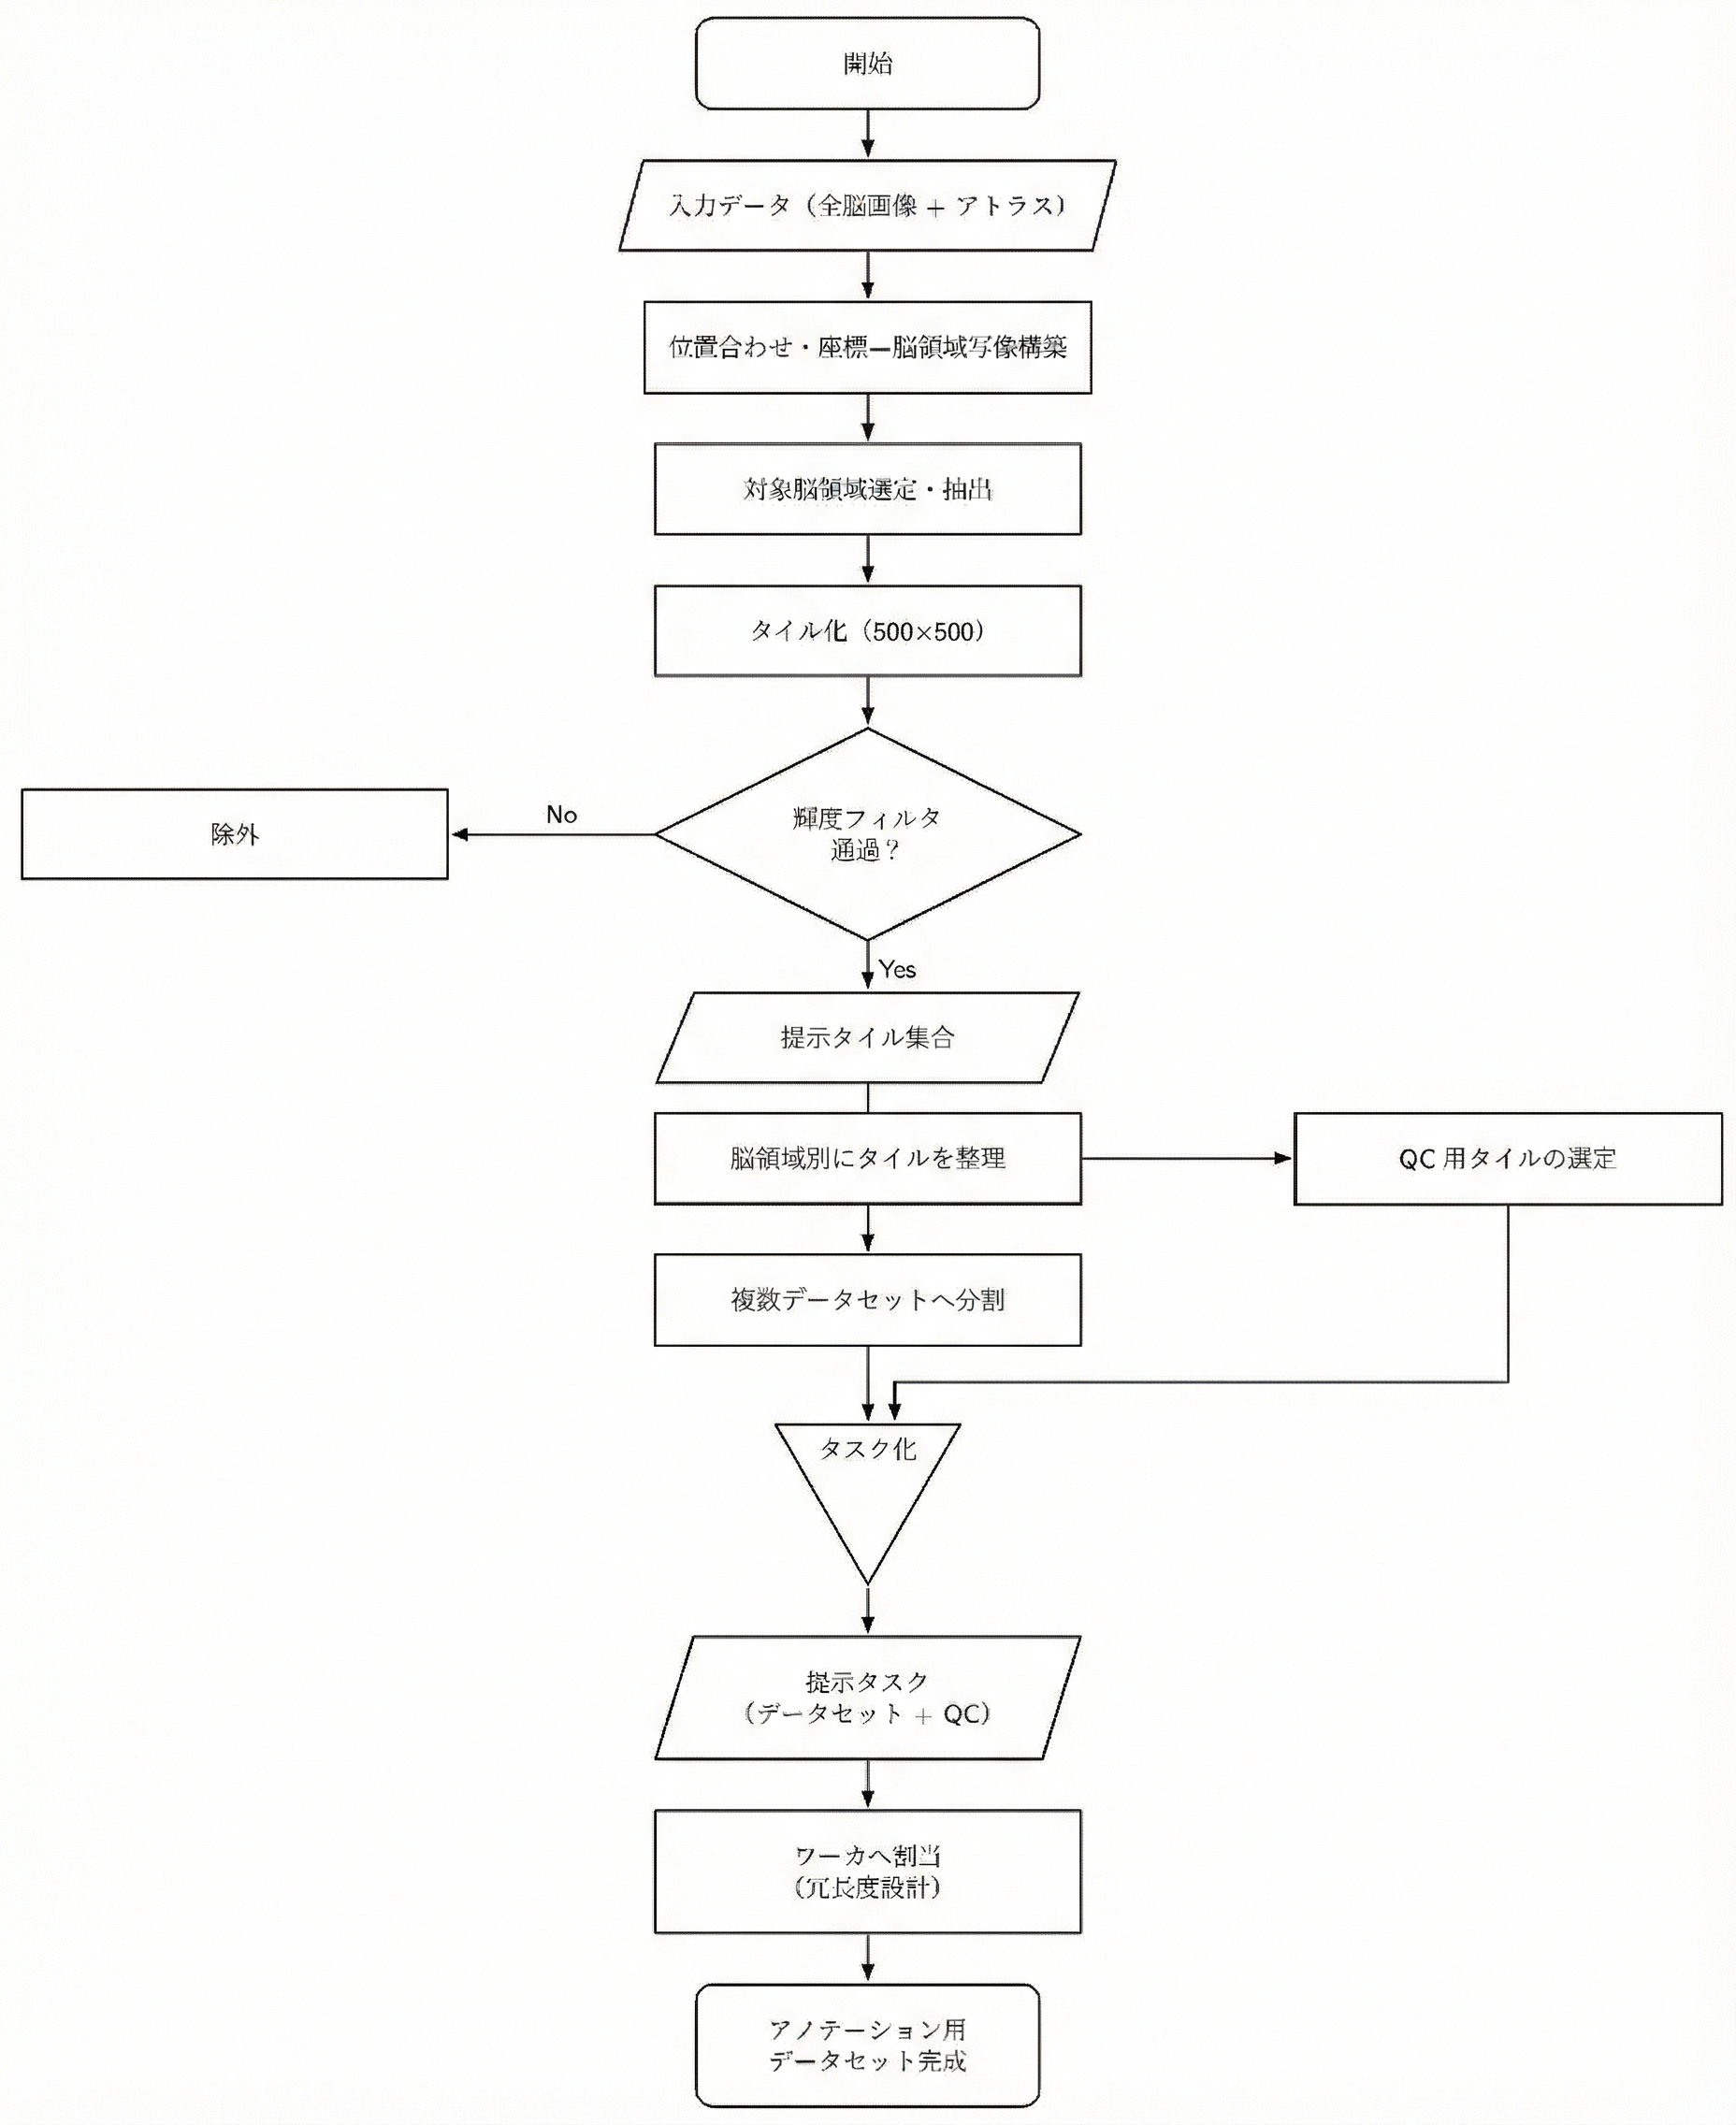
\includegraphics[width=\textwidth, height=0.85\textheight, keepaspectratio]{fig/fig7.png}
  \refstepcounter{figure}\label{fig:fig7}
\end{figure}
\clearpage
本研究におけるクラウドソーシング用アノテーションデータセットの構成手順を示した.全脳画像とマウス脳アトラスを対応付け,座標—領域写像テーブルを構築した.先行研究でArc系シグナルの観察が報告される領域を参照し,Isocortex,olfactory areas,hippocampal formation,cortical subplate,striatumの5領域を抽出対象とした.領域別画像集合を格子状にクロップし,提示単位として500×500タイル画像を生成した.輝度分布に基づくフィルタリングを適用し,極端に暗い/情報量の乏しいタイルを除外した.得られたタイル集合を領域別に整理し,複数のデータセットへ分割してワーカ担当を割り当てた.全ワーカに共通して提示する品質管理用タイルを別途用意し,タスクへ付加した.データセットと品質管理用タイルを統合して提示タスクを構成し,冗長度設計にもとづきワーカへ割り当てた.



\clearpage

\figsubsection{図8 アノテーション収集用Webアプリケーションの画面}
\begin{figure}[h!]
  \centering
  \includegraphics[width=\textwidth, height=0.85\textheight, keepaspectratio]{fig/fig8.png}
  \refstepcounter{figure}\label{fig:fig8}
\end{figure}
\clearpage
アノテーション収集用Webアプリケーションの(a) ホーム画面.(b) 検出画面.(c) ユーザーに示されたインストラクションの例.(d) 管理者用ページの例,ここでは画像に行われたアノテーションの回数などを確認できる.

\clearpage

\figsubsection{図9 アノテーション収集用Webアプリケーションの概念図}
\begin{figure}[h!]
  \centering
  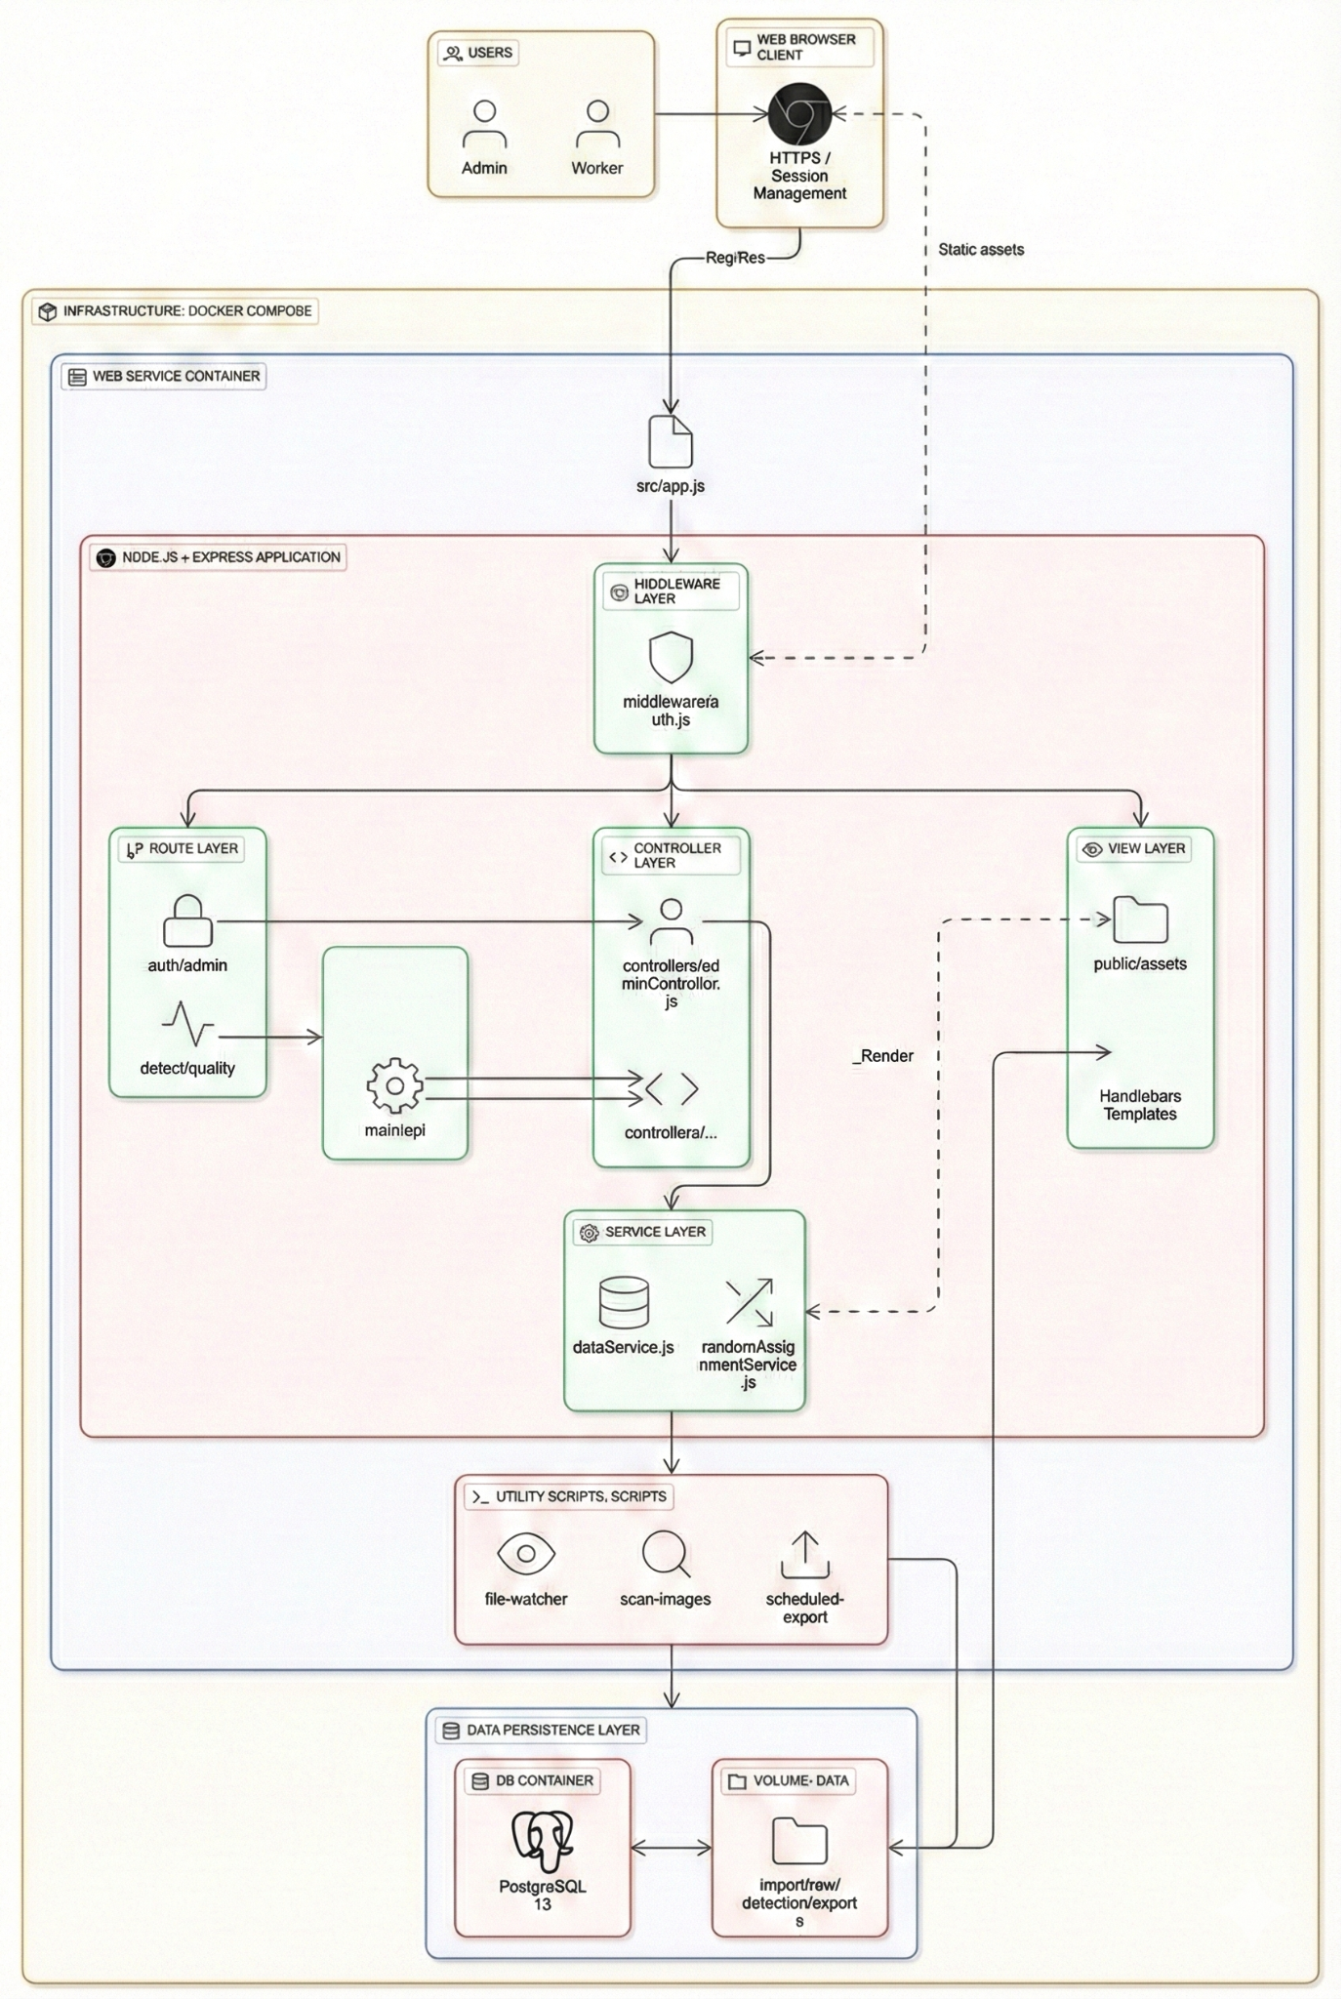
\includegraphics[width=\textwidth, height=0.85\textheight, keepaspectratio]{fig/fig9.png}
  \refstepcounter{figure}\label{fig:fig9}
\end{figure}
\clearpage
システムはDocker Composeにより管理されるコンテナ仮想化環境上で動作する。システム全体は、Webサービスコンテナ、データベースコンテナ(PostgreSQL 13)、およびデータ永続化ボリュームから構成される。 中核となるNode.jsおよびExpressアプリケーションは、保守性と拡張性を確保するため、Middleware、Route、Controller、Service、Viewの各層に責務を分割したレイヤードアーキテクチャを採用した。ユーザー(管理者およびアノテーター)からのリクエストはHTTPSセッションを通じて処理され、Service Layerを介してデータベースやファイルシステムとの入出力が行われる。また、Utility Scripts層により、ファイルの監視や画像スキャン、データのエクスポートなどのバックグラウンド処理が実行される。

\clearpage

\figsubsection{図10 アノテーションのクラスタリング}
\begin{figure}[h!]
  \centering
  \includegraphics[width=\textwidth, height=0.85\textheight, keepaspectratio]{fig/fig10.png}
  \refstepcounter{figure}\label{fig:fig10}
\end{figure}
本研究におけるクラスタ分割手順の可視化例を示した.(a) 点アノテーション集合に対する HDBSCAN のクラスタリング出力のオーバーレイ表示を示した.(b) (a)で得られた単一クラスタの一例に対し,Gaussian mixture model(GMM)による追加分割を適用し,分割後クラスタを色分けしてオーバーレイ表示した.高密度領域における複数細胞の単一クラスタへの併合を抑制した.


\clearpage

\figsubsection{図11 ワーカ能力推定の流れ}
\begin{figure}[h!]
  \centering
  \includegraphics[width=\textwidth, height=0.85\textheight, keepaspectratio]{fig/fig11.png}
  \refstepcounter{figure}\label{fig:fig11}
\end{figure}
\clearpage
図11 複数ワーカの点アノテーションを統合し,細胞中心位置の確信度を画素ごとに表す統合 Ground Truth(確信度付きヒートマップ $\hat{H}$)を生成する処理手順を示す.はじめにワーカ間の不一致を考慮して各候補が真の細胞である確率を推定し,その確率にもとづく重み付きガウス加算によって点集合を連続的なヒートマップへ変換し,正規化・飽和変換を経て学習に用いる $\hat{H}$ を得る.

\clearpage

\figsubsection{図12 アノテーションの点のヒートマップへの変換}
\begin{figure}[h!]
  \centering
  \includegraphics[width=\textwidth, height=0.85\textheight, keepaspectratio]{fig/fig12.png}
  \refstepcounter{figure}\label{fig:fig12}
\end{figure}
点アノテーションから重み付きヒートマップへの変換例.同一タイル領域に対する(a) 収集した全クリック点のオーバーレイ.(b) 推定したワーカ重み $w_{a_i}$ を適用したオーバーレイ.(c) 作成されたGTヒートマップ

\clearpage

\figsubsection{図13 フィルタリングにより分別されたタイル画像}
\begin{figure}[h!]
  \centering
  \includegraphics[width=\textwidth, height=0.85\textheight, keepaspectratio]{fig/fig13.png}
  \refstepcounter{figure}\label{fig:fig13}
\end{figure}
品質フィルタによるタイル画像の選別例.全脳画像から切り出したタイルに対し,輝度ヒストグラムに基づく判定(背景比 $r_{\mathrm{bg}}$,輝度標準偏差 $\sigma_I$,高輝度比 $r_{\mathrm{bright}}$)を適用し,解析対象として採用されたタイル(PASSED,上段)と除外されたタイル(FAILED,下段)の代表例を示す.

\clearpage

\figsubsection{図14 Quality Control画像におけるアノテーションの変換の例}
\begin{figure}[h!]
  \centering
  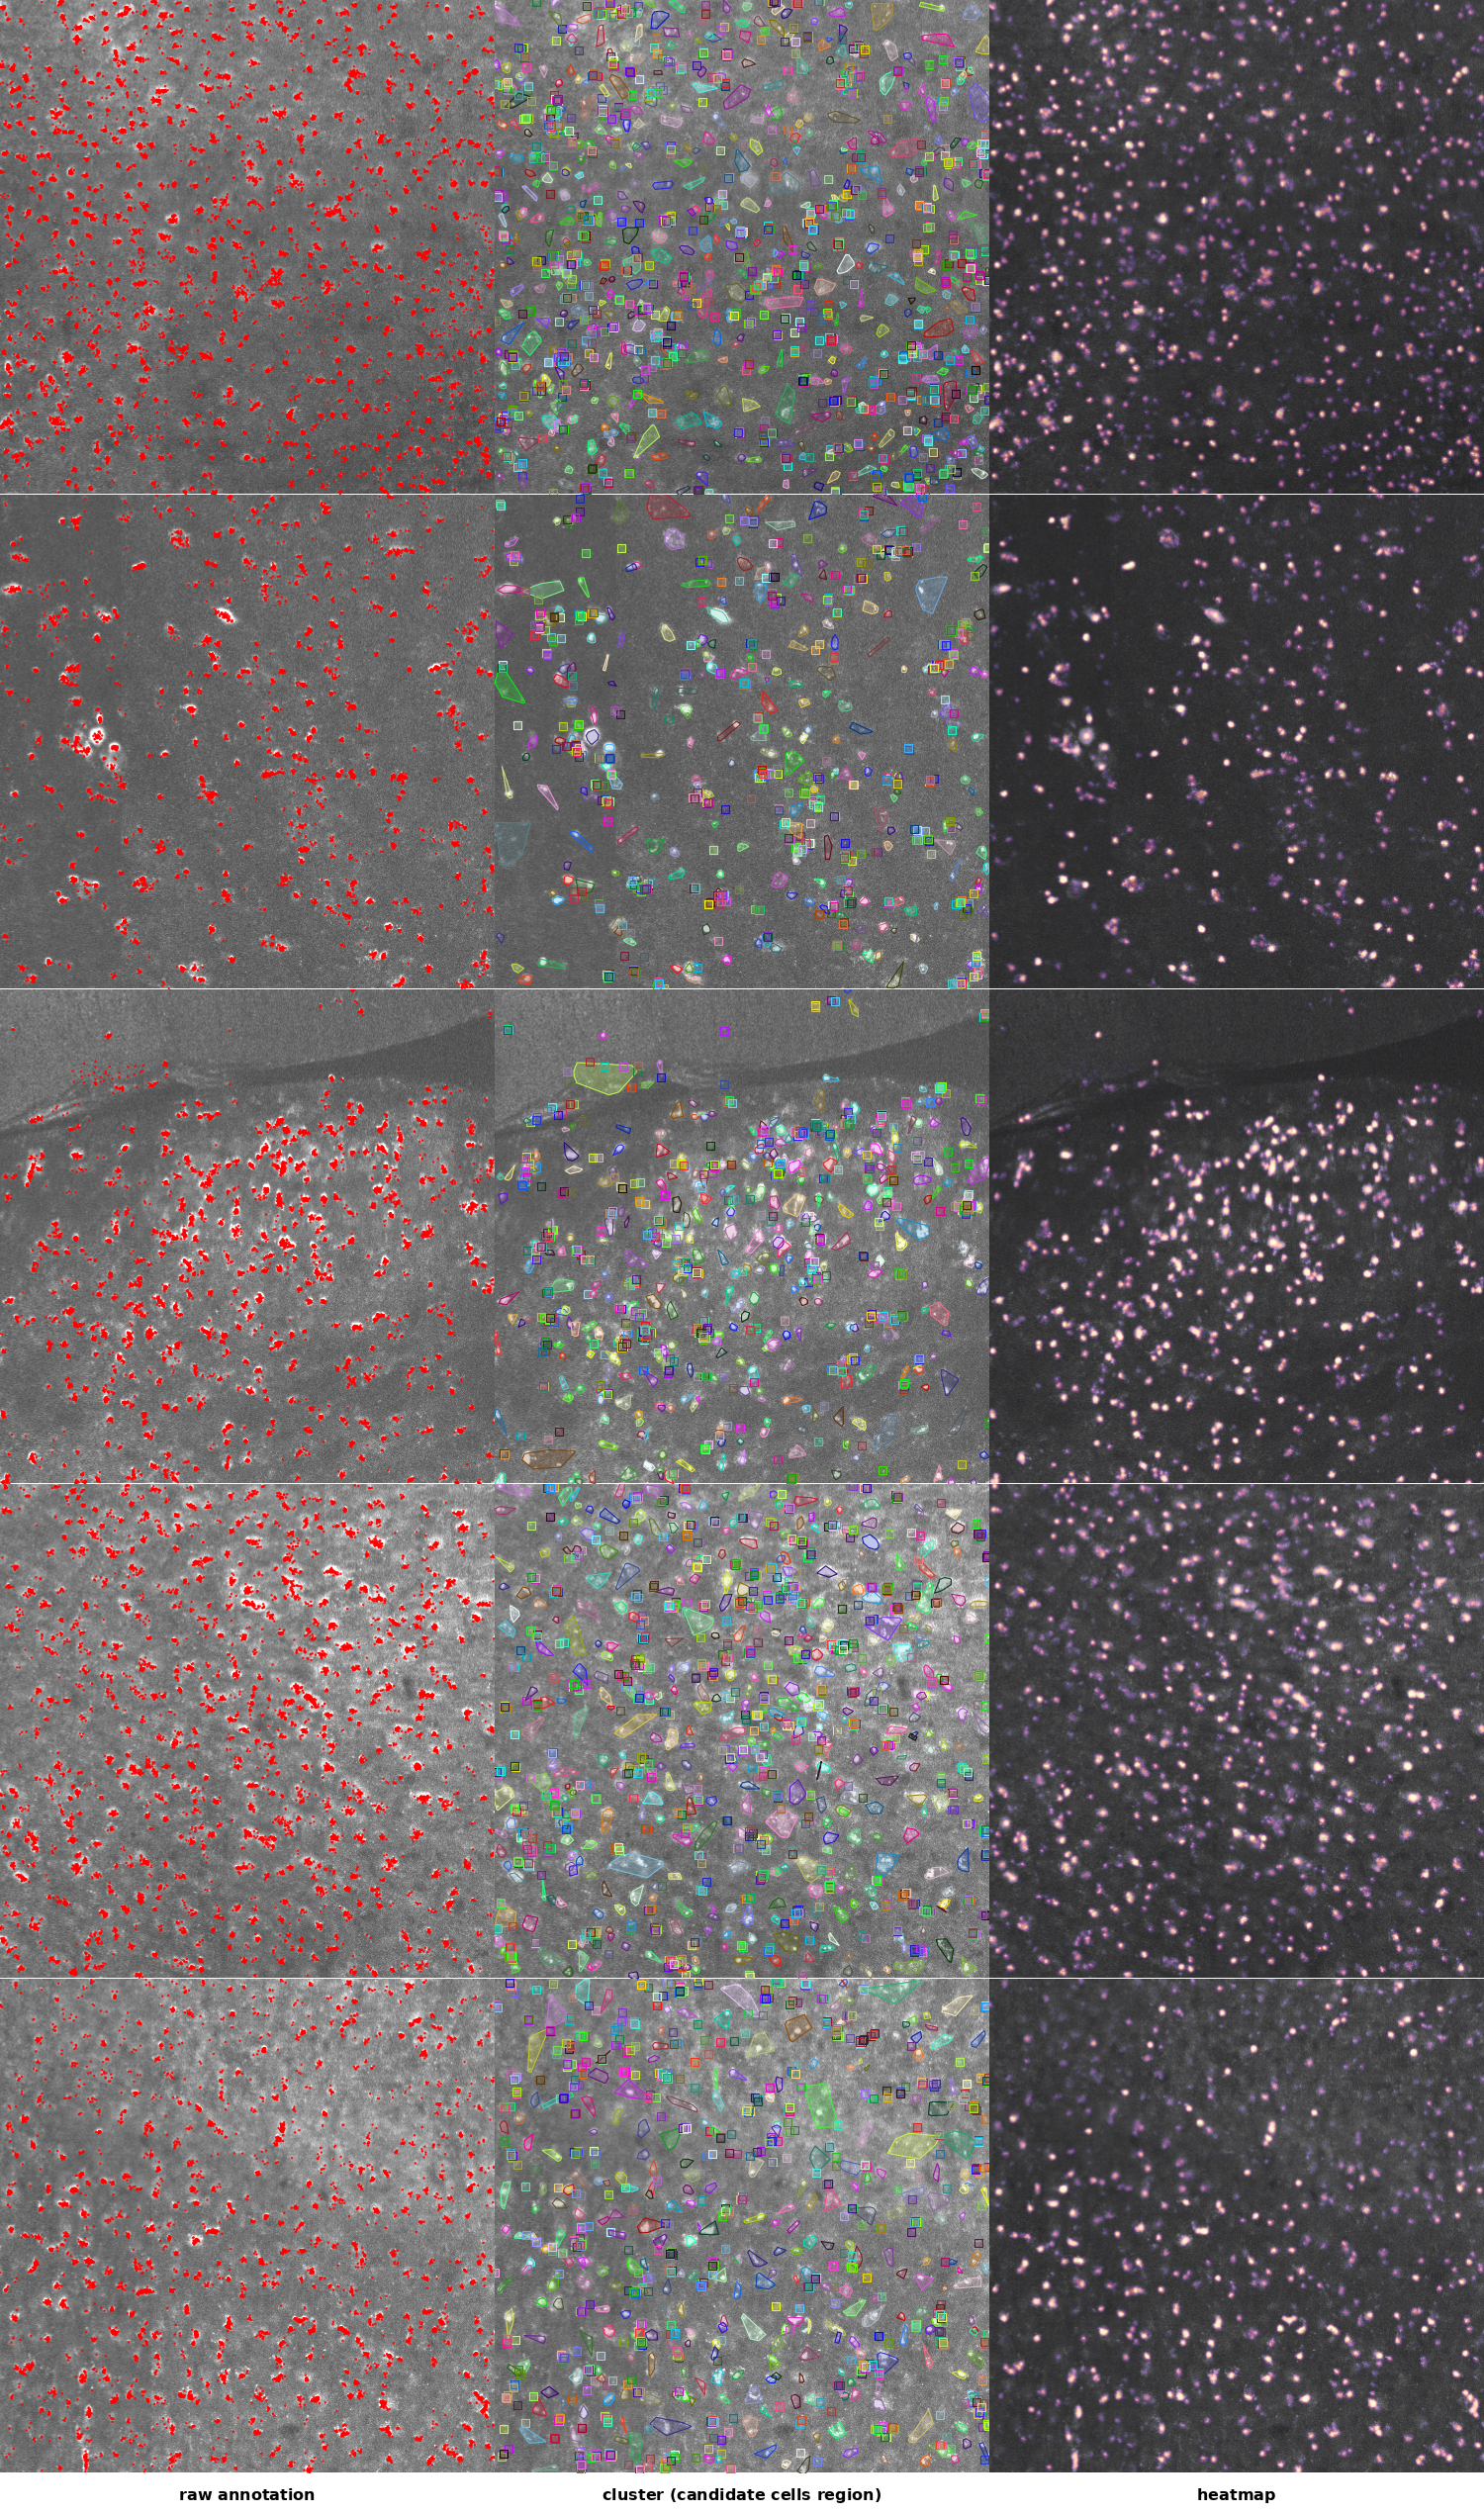
\includegraphics[width=\textwidth, height=0.85\textheight, keepaspectratio]{fig/fig14.png}
  \refstepcounter{figure}\label{fig:fig14}
\end{figure}
\clearpage
本図は,細胞中心点アノテーションの統合処理における各段階の可視化例を示す.左は処理前に収集した全アノテーションの単純なオーバーレイ,中央はクラスタリング後に得られた細胞候補内のアノテーションの凸包の図示(色はクラスタごとにランダムに決定),右は統合処理後のヒートマップのオーバーレイである.

\clearpage

\figsubsection{図15 ワーカの感度,特異度の推定値,ワーカの重み分布}
\begin{figure}[h!]
  \centering
  \includegraphics[width=\textwidth, height=0.85\textheight, keepaspectratio]{fig/fig15.png}
  \refstepcounter{figure}\label{fig:fig15}
\end{figure}
推定されたワーカ感度・特異度の分布と相互関係.(a) 感度の分布と各ワーカの値.破線は平均を示す.(b) 特異度の分布と各ワーカの値.破線は平均を示す.(c) 感度と特異度の散布図.破線は対角線を示す.

\clearpage

\figsubsection{図16 ワーカの重み分布}
\begin{figure}[h!]
  \centering
  \includegraphics[width=\textwidth, height=0.85\textheight, keepaspectratio]{fig/fig16.png}
  \refstepcounter{figure}\label{fig:fig16}
\end{figure}
\clearpage
推定されたワーカ重みの分布と,感度・特異度との対応.(a) 正例側重み(Positive LLR)のカーネル密度推定と各ワーカの値.破線は平均(3.48)を示す.(b) 負例側重み(Negative LLR)のカーネル密度推定と各ワーカの値.破線は平均(−1.12)を示す.(c) 感度と特異度の散布図を正例側重みで着色したもの.(d) 感度と特異度の散布図を負例側重みで着色したもの.(e) ワーカの正例側重み負例側重みの散布図(灰色点:非専門家,赤星:アノテーションの評価において参照した専門家,青破線:線形回帰),重み間の正の相関(Pearson $r=0.664$).


\clearpage

\figsubsection{図17 アノテーション量の偏りと一貫性}
\begin{figure}[h!]
  \centering
  \includegraphics[width=\textwidth, height=0.85\textheight, keepaspectratio]{fig/fig17.png}
  \refstepcounter{figure}\label{fig:fig17}
\end{figure}
QC画像におけるアノテーション量の一貫性に基づくワーカ群分けと,各群のアノテーション密度.(a) $r_w$(各QC画像で $n_{iw}>\bar{n}_i$ を満たす割合)に基づく3群(Below, Mixed, Above)のワーカ数.(b) 1枚あたり平均アノテーション数 $n_w^{\mathrm{img}}=(\sum_i n_{iw})/5$ の群別分布(箱ひげ図).各群のサンプル数(Below: n=20, Mixed: n=3, Above: n=13)を併記した.

\clearpage

\figsubsection{図18 アノテーション量と推定値の関係}
\begin{figure}[h!]
  \centering
  \includegraphics[width=\textwidth, height=0.85\textheight, keepaspectratio]{fig/fig18.png}
  \refstepcounter{figure}\label{fig:fig18}
\end{figure}
QC画像における総アノテーション数と推定能力値(感度・特異度)の関係.(a) 総アノテーション数 $N_w$ と感度の散布図.(b) 総アノテーション数 $N_w$ と特異度の散布図.(c)総アノテーション数 $N_w$ と正例側重みの散布図.(d)総アノテーション数 $N_w$ と負例側重みの散布図.赤破線は線形回帰直線を示し,図中の $r$ は Pearson 相関係数を示す.

\clearpage

\figsubsection{図19 アノテーションから変換されたヒートマップ}
\begin{figure}[h!]
  \centering
  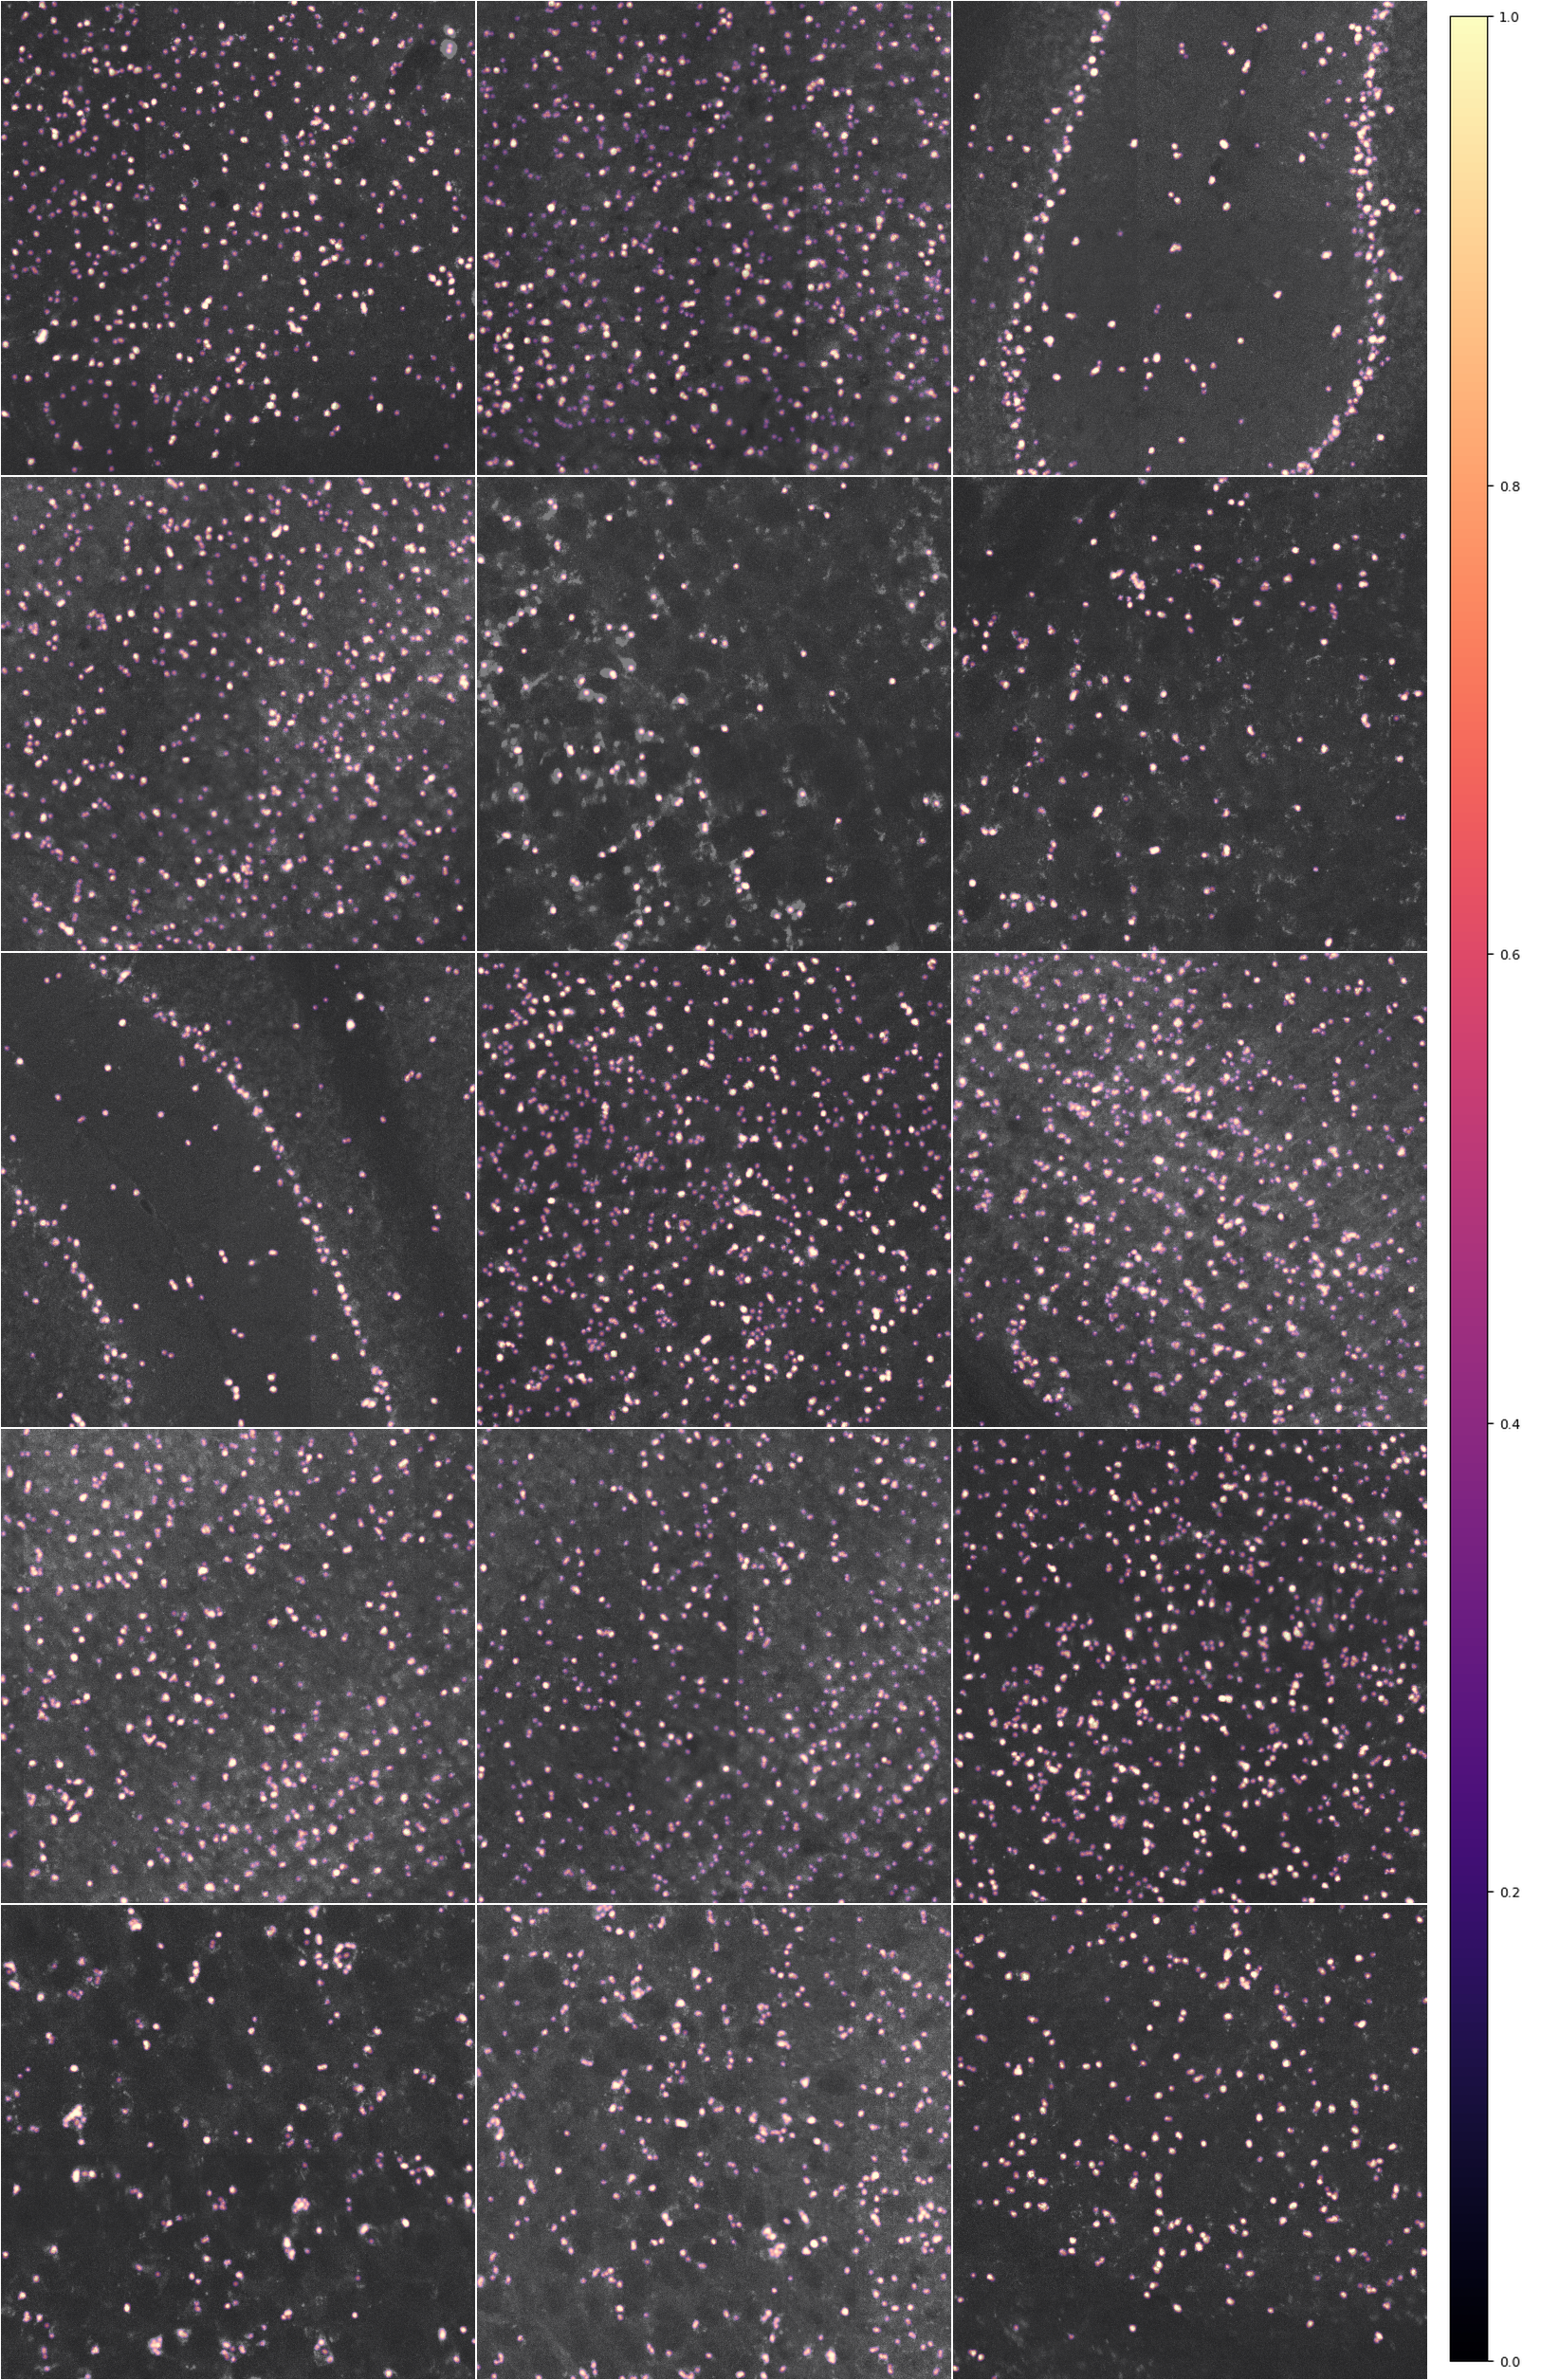
\includegraphics[width=\textwidth, height=0.85\textheight, keepaspectratio]{fig/fig19.png}
  \refstepcounter{figure}\label{fig:fig19}
\end{figure}
\clearpage
推定されたワーカの重みに基づくヒートマップ Ground Truth の例.各小図は解析対象タイルの元画像に,クリック点 $p_i$ をワーカ重み $w_{a_i}$ で加重し,ガウスカーネル $K_\sigma$($\sigma=2.0$ pixel,半径 $2.5\sigma$ で打ち切り)で畳み込んで得たヒートマップ $H$ を重畳したものである.$H$ は非負にクリップ($clip\_min=0.0$)した後,最大値で正規化して $0–1$ に揃えた.色(紫)が強いほど,当該画素が細胞中心点である確率が高いことを示す.複数タイルにわたる代表例を示した.

\clearpage

\figsubsection{図20 合成画像と,生成されるGround Truthの例}
\begin{figure}[h!]
  \centering
  \includegraphics[width=\textwidth, height=0.85\textheight, keepaspectratio]{fig/fig20.png}
  \refstepcounter{figure}\label{fig:fig20}
\end{figure}
\clearpage
生成器による合成タイル画像と中心点 Ground Truth の出力例.左列は生成された合成タイル画像に,対応する細胞重心座標(中心点)を点としてオーバーレイした可視化である.右列は,同一の重心座標列を局所カーネル配置によりヒートマップへ変換した例であり,色が強いほど中心点尤度が高いことを示す.複数タイルにわたる代表例を示した.

\clearpage

\figsubsection{図21 合成画像と実画像データの比較}
\begin{figure}[h!]
  \centering
  \includegraphics[width=\textwidth, height=0.85\textheight, keepaspectratio]{fig/fig21.png}
  \refstepcounter{figure}\label{fig:fig21}
\end{figure}
\clearpage
合成タイル画像とアノテーション由来実画像タイルの統計的比較.生成器による合成タイル画像 $N=170$ 枚(PNG)と重心座標ファイル $N=170$ 個(JSON)を,アノテーション由来の実画像タイル $N=170$ 枚(PNG)と中心点ヒートマップ $N=170$ 枚(NumPy 配列)と比較し,同一の記述統計量および可視化指標を算出した.(A) 各タイルの平均輝度分布.(B) 各タイルの画素輝度標準偏差(コントラスト指標)の分布.(C) 全タイルの画素輝度ヒストグラム.(D) 中心点近傍を除外して定義した背景画素のみの輝度ヒストグラムと.(E) Fourier 変換に基づく放射平均パワースペクトル(平均).(F–H) 局所テクスチャ統計の比較として,Laplacian 分散(F),勾配強度(G),Shannon エントロピー(H)のヒストグラム.(I) Ground Truth が指示する領域と背景の平均輝度差(signal $-$ background)の分布.(J) タイル輝度統計とテクスチャ特徴からなる特徴空間において,合成タイル各例に対する最近傍の実画像タイルを対応付けて並置した例,奇数列目は合成画像で,それぞれの右に位置する画像が最近傍の実画像.

\clearpage

\figsubsection{図22 専門家のアノテーションと統合されたアノテーションの整合評価}
\begin{figure}[h!]
  \centering
  \includegraphics[width=\textwidth, height=0.85\textheight, keepaspectratio]{fig/fig22.png}
  \refstepcounter{figure}\label{fig:fig22}
\end{figure}
(a) 統合ヒートマップ $H^{\text{agg}}$ の閾値 $\theta$ を掃引して得た Precision–Recall 曲線(Expert Excluded:評価対象の専門家を統合から除外,Expert Included:評価対象の専門家を統合に含める).プロット上の各点は異なる $\theta$ 値に対応する値であり,指標は48枚×2名専門家の全ペアで micro-average により算出.(b) 閾値 $\theta$ 掃引により得た FROC 曲線(横軸:1画像あたり偽陽性数,縦軸:Recall).(c) 閾値 $\theta$ に対する $F1$ の変化($F1$ 最大点 $\theta^{\ast}\approx 0.97$,Expert Excluded:$F1=0.541$,Expert Included:$F1=0.708$).(d) 閾値 $\theta$ に対する Precision および Recall の変化.実線はExpert Includedの結果を,点線はExpert Excludedでの結果を表す.


\clearpage

\figsubsection{図23 事前学習モデルとファインチューニングモデルの検出性能比較}
\begin{figure}[h!]
  \centering
  \includegraphics[width=\textwidth, height=0.85\textheight, keepaspectratio]{fig/fig23.png}
  \refstepcounter{figure}\label{fig:fig23}
\end{figure}
\clearpage
3種類の距離許容閾値($\tau = 3, 5, 7$ピクセル)におけるPrecision-Recall曲線を示す.各行は特定の$\tau$値に対応し,赤線はモデルPを,青線はモデルTを表す.
モデルTは全ての距離閾値においてモデルPを上回り,特に$\tau = 3\text{px}$では+37.8\%のAUPRC向上を示した.

\clearpage

\figsubsection{図24 Ground Truth確信度とモデル出力確信度の整合性}
\begin{figure}[h!]
  \centering
  \includegraphics[width=\textwidth, height=0.85\textheight, keepaspectratio]{fig/fig24.png}
  \refstepcounter{figure}\label{fig:fig24}
\end{figure}
\clearpage
左列(a–d):モデルP(事前学習),右列(e–h):モデルT(ファインチューニング)(a, e) タイルごとの予測ヒートマップ最大値の分布.モデルPは低い確信度スコアを出力(中央値 = 0.678)するのに対し,モデルTは高い値(中央値 $\approx 1.0$)を出力する.(b, f) マッチしたピークペアにおける予測確信度とGT確信度の散布図.モデルTはモデルP($r = 0.240$)より高い相関($r = 0.419$)を示す.(c, g) 予測確信度とGT確信度のキャリブレーションを示す信頼性図.対角線は完全なキャリブレーションを表す.モデルTはモデルP(Brier = 0.532)と比較して大幅に改善(Brier = 0.117)している.(d, h) GT確信度区間ごとのRecall.モデルTは明確な単調関係を示す:GT確信度が高いほど検出確率が高い(GT確信度0.9–1.0でRecall = 0.935).

\clearpage

\figsubsection{図25 GT閾値($\theta_{\text{gt}}$)と予測閾値($\theta$)の2次元パラメータ掃引解析}
\begin{figure}[h!]
  \centering
  \includegraphics[width=\textwidth, height=0.85\textheight, keepaspectratio]{fig/fig25.png}
  \refstepcounter{figure}\label{fig:fig25}
\end{figure}
\clearpage
左列(a–c):F1スコアヒートマップ,右列(d–f):閾値最適化曲線 (a) モデルPのF1ヒートマップ($\tau = 5\text{px}$).高F1領域は$\theta_{\text{gt}} \approx 0.70\text{--}0.75$,$\theta \approx 0.025$の狭い帯域に限定され,F1 $\ge 0.60$を達成する格子点は2点のみ.(b) モデルTのF1ヒートマップ($\tau = 5\text{px}$).高F1領域が大幅に拡大し,F1 $\ge 0.70$を達成する格子点は26点に増加.閾値選択に対するロバスト性の向上を示す.(c) モデルTのF1ヒートマップ($\tau = 7\text{px}$).距離許容度の緩和により同様のパターンを示し,最大F1 = 0.741を達成.(d) モデルPにおける,$\theta_{\text{gt}}$に対する達成可能な最大F1.最適値から離れると性能が急速に低下する.(e) モデルTにおける,$\theta_{\text{gt}}$に対する達成可能な最大F1.$\theta_{\text{gt}} \in [0.3, 0.6]$の広い範囲で高F1のプラトーが存在.(f) モデルTにおける,$\theta_{\text{gt}}$に対する最適予測閾値$\theta^*$.モデルPでは$\theta^*$が一定のままであるのに対し,モデルTでは$\theta_{\text{gt}}$の増加に伴い$\theta^*$も単調増加し,GTと予測確信度スケールの対応関係の学習を示唆.

\clearpage

\figsubsection{図26 検出モデル出力の変化(閾値低)}
\begin{figure}[h!]
  \centering
  \includegraphics[width=\textwidth, height=0.85\textheight, keepaspectratio]{fig/fig26.png}
  \refstepcounter{figure}\label{fig:fig26}
\end{figure}
\clearpage
アノテーション由来のGround Truthデータセットから,大脳皮質のタイルに対し,モデルP(事前学習モデル)およびモデルT(ファインチューニングモデル)の出力を比較したものである.検出閾値を0.05,0.40,0.90と変化させ,閾値設定がモデル間の検出挙動に与える影響を可視化した.

各図のレイアウトは以下の通りである.
1行目左は元画像,1行目右はGTヒートマップ(オーバーレイ表示,viridisカラーマップ)を示す.
2行目左はモデルPの検出点(赤点,閾値以上のピーク),2行目右はモデルPの予測ヒートマップ(正規化後オーバーレイ)である.
3行目左はモデルTの検出点(青点,閾値以上のピーク),3行目右はモデルTの予測ヒートマップ(正規化後オーバーレイ)である.
4行目左はモデルPの検出点をGTヒートマップ上にオーバーレイしたもの,4行目右はモデルTの検出点をGTヒートマップ上にオーバーレイしたものである.

各パネル右端のカラーバーは,当該行のヒートマップの確信度スケールを示す.
2行目(モデルP)は最大値が約0.7程度と低いため,カラーバーのスケールが他行と異なる.低閾値では両モデルとも多数の候補点を出力するが,偽陽性も多く含まれる.中程度の閾値では,モデルPの検出点はほぼ消失する一方,モデルTは依然として多くの検出点を維持している.高閾値では,モデルPは検出点が皆無となり,モデルTのみが高確信度の検出点を出力する.

\clearpage

\figsubsection{図27 検出モデル出力の変化(閾値中)}
\begin{figure}[h!]
  \centering
  \includegraphics[width=\textwidth, height=0.85\textheight, keepaspectratio]{fig/fig27.png}
  \refstepcounter{figure}\label{fig:fig27}
\end{figure}
\clearpage

\figsubsection{図28 検出モデル出力の変化(閾値高)}
\begin{figure}[h!]
  \centering
  \includegraphics[width=\textwidth, height=0.85\textheight, keepaspectratio]{fig/fig28.png}
  \refstepcounter{figure}\label{fig:fig28}
\end{figure}

\clearpage

\figsubsection{図29 FASTdシステムの概要}
\begin{figure}[h!]
  \centering
  \includegraphics[width=\textwidth, height=0.85\textheight, keepaspectratio]{fig/fig29.png}
  \refstepcounter{figure}\label{fig:fig29}
\end{figure}
FASTd は,スピニングディスク共焦点顕微鏡,自動リニアスライサー,電動ステージの三要素から構成される.撮像時には,スピニングディスク共焦点顕微鏡が各切片に対して複数の FOV を順次撮像し,その切片に含まれる全ての FOV の撮像が完了した時点で,自動リニアスライサーが次の切片層を切断する.この手順を反復することで,連続的な断層撮像を実現している.

\clearpage

\figsubsection{図30 FASTdにより撮像された脳画像の例}
\begin{figure}[h!]
  \centering
  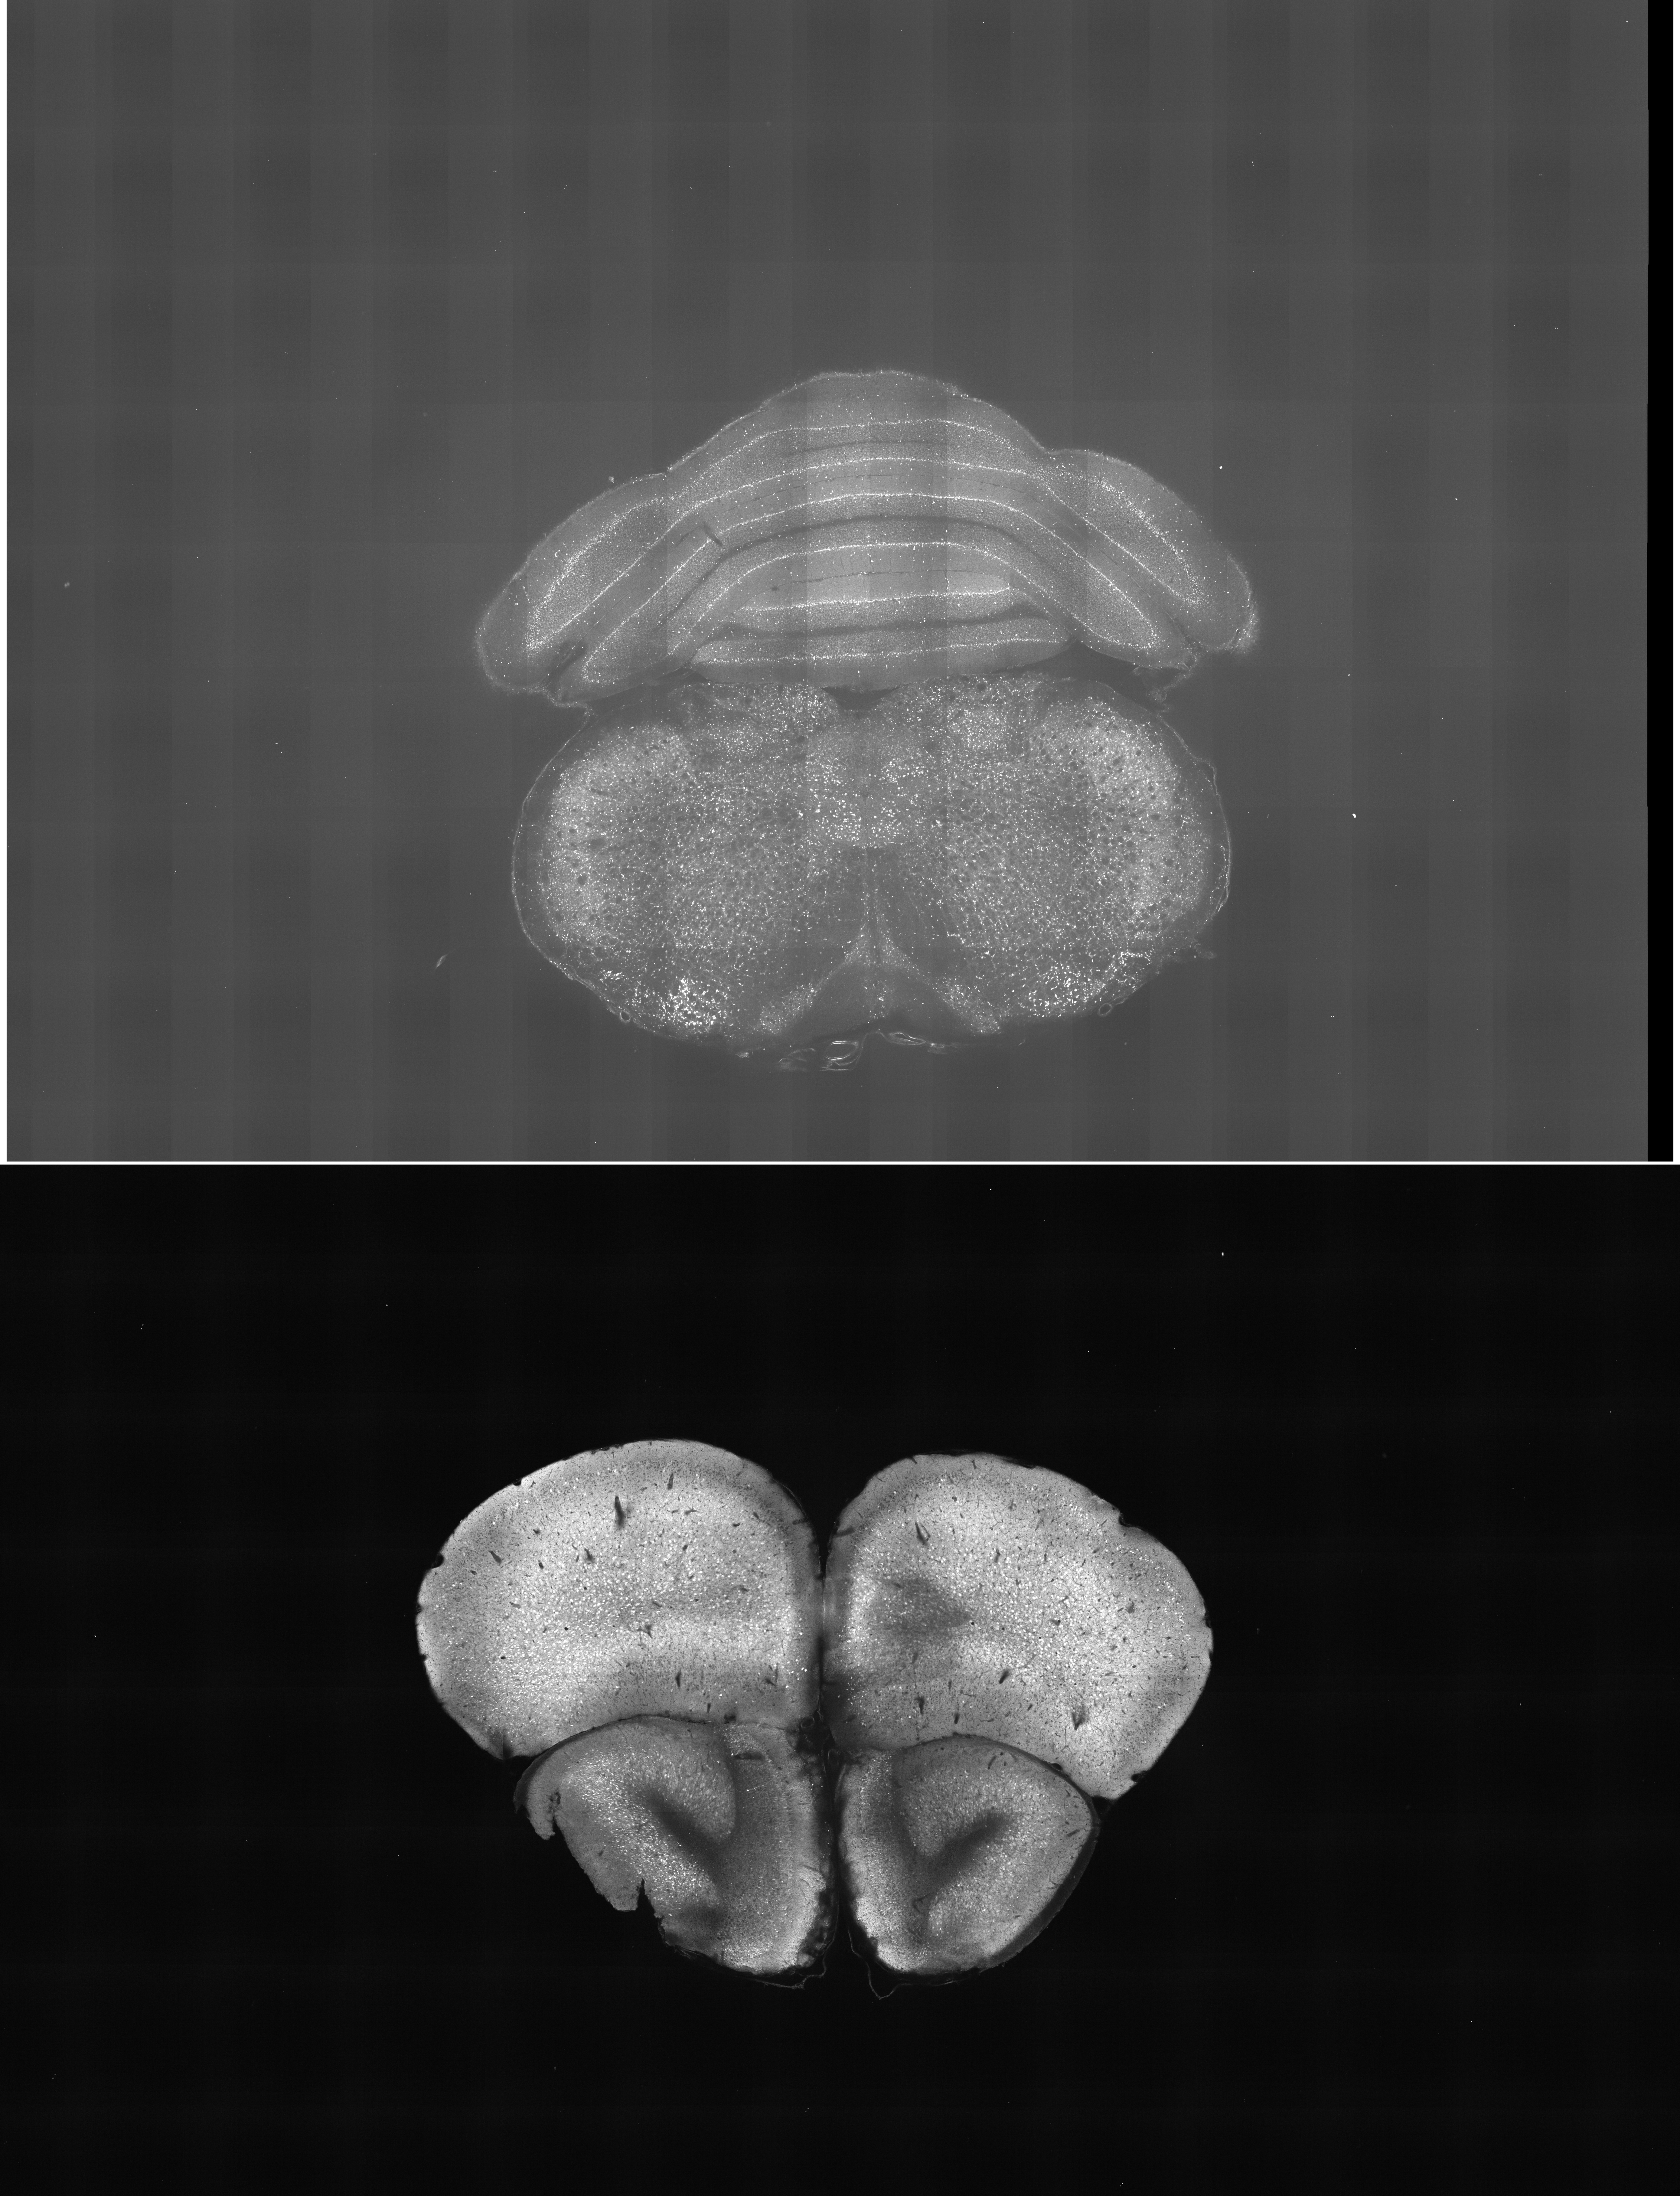
\includegraphics[width=\textwidth, height=0.65\textheight, keepaspectratio]{fig/fig30.png}
  \refstepcounter{figure}\label{fig:fig30}
\end{figure}
FASTd により撮像されたマウス全脳蛍光画像の例を示す.上は FL3/RFP マウスの画像,下は Arc-dVenus マウスの画像であり,いずれも撮像画像の輝度を正規化する処理を加えたもの.
% --- 参考文献 ---
\newpage
\nocite{*}
\printbibliography[title=引用文献, heading=bibintoc]
% --- 謝辞 ---
\clearpage
\section*{謝辞}
\addcontentsline{toc}{section}{謝辞}
本研究を遂行するにあたり,研究環境を提供してくださった京都大学大学院,生命科学研究科 高次生命科学専攻,脳機能発達再生制御学分野の今吉格教授に深く感謝申し上げます.多大なるご指導と適切な助言を賜り,研究を円滑に進めることができました.また,懇切丁寧なご指導と幅広い助言を頂戴した鈴木裕輔助教にも心より感謝いたします.さらに,進捗報告会や日々の研究室活動において多くの貴重なアドバイスを頂いた山田真弓特定准教授, Adam T. Guy 准教授,坂本雅行准教授,道川貴章特定准教授,長崎真治助教,横山達士助教にも深く御礼申し上げます.加えて,アノテーションツールを用いた細胞アノテーションを通じて研究に参加してくださった方々に,この場を借りて厚く御礼申し上げます.そして,日々の有益な議論や研究活動を通じて多大な支援を頂いた脳機能発達再生制御学研究室の皆様にも心より感謝申し上げます.京都大学大学院 生命科学研究科 博士課程 3 年の行天悠一郎さん,同修士課程2年の根本直広さん,山本泰生さんには,実験データの提供やアノテーションツールのテストにおいて多大なるご協力をいただき,深く感謝いたします.

\section*{研究で使用したコードの公開}
\addcontentsline{toc}{section}{研究で使用したコードの公開}
\noindent 本研究で開発したソースコードは,GitHub上で公開している.
\\
\url{https://github.com/h1s4gi0rc4/}

\section*{連絡先}
\addcontentsline{toc}{section}{連絡先}
okada.yuuma.77m@st.kyoto-u.ac.jp

\end{document}